% !LW recipe = Paper (portable)
% Build with LaTeX Workshop or `make arxiv`; output: build/main_arxiv.pdf.
\documentclass[11pt,letterpaper]{article}
\usepackage[T1]{fontenc}
\usepackage[margin=1in]{geometry}
\usepackage[round,authoryear]{natbib}
\usepackage{microtype}
\usepackage{amsmath,amssymb,amsfonts,bm}
\usepackage{amsthm}
\usepackage{graphicx,booktabs,multirow,array}
\usepackage[section]{placeins}
\usepackage{hyperref,url}
\usepackage{xcolor}
\hypersetup{colorlinks=true,linkcolor=blue!50!black,citecolor=blue!50!black,urlcolor=blue!60!black}
\raggedbottom
\setlength{\emergencystretch}{2em}
\newcommand{\E}{\mathbb{E}}
\newcommand{\R}{\mathbb{R}}
\newcommand{\sg}{\operatorname{sg}}
\newcommand{\CE}{\operatorname{CE}}
\newcommand{\KL}{\operatorname{KL}}
\newcommand{\LN}{\operatorname{LogitNormal}}
\newcommand{\passk}{\operatorname{pass}@k}
\newcommand{\votek}{\operatorname{vote}@k}
\newcommand{\pending}{\textemdash}
\newcommand{\ours}{CEDR}
\newcommand{\asyncclock}{(2.5,2,1.5)}
\newtheorem{lemma}{Lemma}
\newcommand{\xc}[1]{{\color{black!10!orange} [x: #1]}}

\title{Reasoning with Continuous Latent Diffusion}
\author{Xiang Cheng\\
Duke University\\
Department of Electrical and Computer Engineering\\
\texttt{xiang.cheng@duke.edu}}
\date{}

\begin{document}
\maketitle

\begin{abstract}
We show that continuous diffusion language models can achieve strong reasoning performance by denoising in a learned latent space. In our Continuous Embedding Diffusion Reasoner (CEDR), built on ELF, ablations identify latent representation as a key determinant of reasoning accuracy: accurate decoding alone does not ensure strong generation. We therefore combine learned representations from three hidden layers of Qwen3-4B to balance ease of generation and decoding. This decomposition also enables asynchronous denoising, allowing different components to be refined at different rates. A compact prompt encoder (121M parameters for CEDR-L, excluding token embeddings) replaces the external teacher Transformer at inference while retaining its frozen token embedding table. Adapting DiffusionNFT to learned self-conditioning guidance further demonstrates that established diffusion reinforcement learning techniques can improve the accuracy of continuous reasoning models. With a 638M-parameter denoising backbone, post-NFT CEDR-L achieves 68.97\% pass@1 on GSM8K and 32.40\% on MATH500 at 64 denoising steps, and 40.09\% on HumanEval and 36.74\% on HumanEval+ at 128 denoising steps, using DMD2-style stochastic sampling.
Code will be available at: \url{https://github.com/chengxiang/CEDR}.
\end{abstract}

\section{Introduction}
\label{sec:introduction}

Autoregressive language models have made substantial progress on mathematical reasoning \citep{minerva,deepseekr1}. Continuous diffusion offers a complementary approach: it generates complete solutions by iteratively refining a continuous latent representation of all answer positions. In this work, we investigate the capabilities of continuous diffusion language models on challenging mathematical reasoning and code generation tasks, and the design choices that enable strong performance.

We introduce the Continuous Embedding Diffusion Reasoner (CEDR), based on the simple continuous flow formulation of Embedded Language Flows (ELF; \citealp{elf}). A key design choice is the latent representation, which must capture the complex semantics and dependencies within reasoning solutions while remaining amenable to generation via continuous denoising. Our pipeline learns compact answer representations from three hidden layers of Qwen3-4B \citep{qwen3} (Figure~\ref{fig:pipelineoverview}). A staged curriculum first trains the diffusion model with teacher prompt features, then fits a compact prompt encoder and jointly adapts both networks. The resulting model performs prompt encoding and answer generation without an external contextual encoder, retaining Qwen's frozen token-embedding table for prompt input. Its decomposable answer representation supports both standard synchronous denoising and asynchronous algorithms that refine different components at different rates (Section~\ref{sec:clocks}).

Our supervised CEDR-L exceeds reported comparable-scale continuous-diffusion baselines on mathematical reasoning and code generation (Tables~\ref{tab:headlinecomparison} and~\ref{tab:codingcomparison}). Remaining close to standard continuous diffusion also lets us apply established diffusion reinforcement learning techniques. We adapt DiffusionNFT \citep{diffusionnft} to accommodate learned self-conditioning guidance and show that it can further improve model accuracy, with clear gains on mathematical reasoning (Figure~\ref{fig:headlinestages}).

\paragraph{Contributions.}
\label{sec:contributions}

Our complete reasoning pipeline comprises the following key contributions:

\begin{enumerate}
    \item \textbf{Strong reasoning with continuous latent diffusion.}
    CEDR outperforms recent comparable-sized continuous-diffusion baselines on math and code (Tables~\ref{tab:headlinecomparison}--\ref{tab:headlinelownfe} and~\ref{tab:codingcomparison}).

    \item \textbf{Representation design using multilayer hidden activations of an autoregressive reasoning model.}
    We empirically investigate the tradeoff between preserving reasoning information and ease of generation (Figure~\ref{fig:representationcomparison}). Guided by these findings, we learn compact projections of Qwen's multilayer hidden activations using a decoding cross-entropy loss (Figure~\ref{fig:pipelineoverview}). Our decomposable representation enables asynchronous inference, with separate denoising clocks for different layer components (Section~\ref{sec:clocks}; Table~\ref{tab:inferenceclocks}).

    \item \textbf{Replacing external prompt encoders with a lightweight Transformer.}
    We train a lightweight Transformer to replace Qwen for prompt encoding, removing dependence on an external contextual encoder while retaining Qwen's frozen token-embedding table. Our analysis shows that an ideal denoiser does not require exact Qwen feature matching: its prompt encoder need only preserve the information required to denoise the answer (Lemma~\ref{lem:conditionalrepresentation}). This motivates jointly adapting the prompt encoder and diffusion backbone within our staged training curriculum (Figure~\ref{fig:promptcurriculum}).

    \item \textbf{Guidance-compatible diffusion reinforcement learning for reasoning.}
    We adapt DiffusionNFT \citep{diffusionnft} to work with learned self-conditioning guidance while retaining guided rollouts (Section~\ref{sec:nftsccfg}). Our update uses both model rollouts and gold solutions from the training set. We theoretically characterize the gold contribution as anchoring the learned denoising field toward a blend of the denoising target implied by gold data and the previous policy (Lemma~\ref{lem:goldanchor}).
\end{enumerate}

\section{Related work}
\label{sec:relatedwork}

\textbf{Diffusion language models.} Language diffusion operates in continuous representations \citep{plaid,tess2,hyperspherical} or discrete token spaces \citep{mdlm,llada,dbtm}, with recent continuous models targeting reasoning, coding, and few-step generation \citep{posterior,mlfm,plaidq}. We build on ELF \citep{elf}, which denoises contextual representations and shares a backbone between denoising and token decoding. Concurrent to our paper, ELF-REG \citep{scalingdlm} augments ELF with teacher-feature alignment and a jointly denoised global representation. CEDR learns its answer representation and replaces external prompt encoders with a compact trainable network.
\textbf{Representation design and denoising order.} Related work learns or aligns diffusion representations in vision and language \citep{repa,textldm,ldlm}, and explores separate denoising clocks for representation components in vision \citep{sfd,latentforcing}. We study learned multilayer language representations for both decoding and generation, and use their structure for asynchronous inference. \textbf{Stochastic sampling.} Consistency models alternate clean prediction with fresh noise injection \citep{consistencymodels}, a construction adopted for multi-step generation in DMD2 \citep{dmd2}. EDM adds noise churn before a numerical denoising step \citep{edm}. ELF-REG also evaluates clean-prediction re-noising for continuous language generation \citep{scalingdlm}. We apply these established sampling ideas to asynchronous local clocks (Section~\ref{sec:clocks}).
\textbf{Diffusion reinforcement learning.} Reward-based post-training has also been explored for diffusion reasoning \citep{d1,llada15,ladirl}. We adapt DiffusionNFT \citep{diffusionnft}, which optimizes rewarded endpoints through forward-process regression. Our adaptation accommodates ELF's learned self-conditioning guidance, adds gold-solution anchoring, and jointly updates the flow model and prompt encoder.

\section{Preliminaries}
\label{sec:preliminaries}

\textbf{Tokens, encodings, and latents.}
Let $q=(q_1,\ldots,q_{L_q})$ and $a=(a_1,\ldots,a_{L_a})$ be prompt and answer tokens in vocabulary $\mathcal V$, with the answer including its terminal token. Their padded canvas $y=(q,a,\mathrm{padding})$ has length $L$; canvas index $i$ and answer index $j$ satisfy $y_{L_q+j}=a_j$. An answer encoder gives $z_{\mathrm{clean}}=\mathcal E(q,a)\in\R^{L_a\times d}$, and a prompt-only encoder gives $c_\phi(q)=P_\phi(q)\in\R^{L_q\times d}$; rows are token vectors. Unlike the teacher's tokenwise lookup $B_\psi[q_i]$, $P_\phi$ uses prompt context. Parameters $\psi$ are frozen teacher weights, $\phi$ the prompt encoder, and $\theta$ the shared denoising/decoding network, with $\Theta=(\theta,\phi)$. Teacher layer $\ell$ contributes width $d_\ell$ to total latent width $d$. Uppercase letters denote random variables.

\textbf{Flow matching.}
Flow matching transports noise to data \citep{flowmatching}. For noise scale $\sigma>0$, our linear Gaussian path runs from noise at $t=0$ to clean latents at $t=1$:
\begin{equation}
 z_t=t z_{\mathrm{clean}}+(1-t)\sigma\epsilon,
 \qquad \epsilon\sim\mathcal N(0,I),\qquad
 u_t:=\frac{\mathrm d z_t}{\mathrm d t}=z_{\mathrm{clean}}-\sigma\epsilon.
 \label{eq:methodinterpolant}
\end{equation}
Treating text $q$ as the external condition and $c_\phi(q)$ as its internal encoding, write $v_\Theta(z,t;q):=v_\theta(z,t;c_\phi(q))$. The conditional objective is
\begin{equation}
 \mathcal L_{\mathrm{FM}}^{\mathrm{basic}}(\Theta)
 =\E\!\left[\left\|v_\theta\bigl(z_t,t;c_\phi(q)\bigr)-u_t\right\|_F^2\right].
 \label{eq:basicflowloss}
\end{equation}
The expectation samples training pairs $(q,a)$, times $t\sim\pi(t)$, and independent Gaussian noise.

\textbf{Text and encoded conditioning.}
Write $p_t(z\mid q)$ for the forward-path density and $s^\star(z,t\mid q)=\nabla_z\log p_t(z\mid q)$ for its conditional score. For $0<t<1$, the population-optimal velocity is
\begin{equation}
 v^\star(z,t\mid q)
 =\E[u_t\mid z_t=z,q]
 =\frac{z+\sigma^2(1-t)s^\star(z,t\mid q)}{t}.
 \label{eq:conditionalflowscore}
\end{equation}
Conditioning on $c_\phi(q)$ may merge distinct prompts; Section~\ref{sec:conditionalencoding} characterizes when the encoding preserves the text-conditional score.

\textbf{Sampling under a different clock.}
At inference, let $\tau\in[0,1]$ be solver time and $t=f(\tau)$ an increasing differentiable clock with $f(0)=0$, $f(1)=1$. Starting from $\bar z_0\sim\mathcal N(0,\sigma^2I)$, sampling obeys $\mathrm d\bar z_\tau/\mathrm d\tau=f'(\tau)v_\Theta(\bar z_\tau,f(\tau);q)$. For $f(\tau)=\tau^2$, the multiplier is $2\tau$. Exact integration preserves the endpoint, while finite-step accuracy can change. Section~\ref{sec:clocks} extends this to group-specific clocks.

% BEGIN continuous diffusion framework and design choices
\section{Continuous Diffusion Reasoning}
\label{sec:methodology}
\label{sec:methodflow}

For a general, fixed answer representation $\mathcal E(q,a)$ and prompt encoding $c=c(q)$, CEDR follows ELF's denoising and token-decoding formulation~\citep{elf} (Figure~\ref{fig:pipelineoverview}). We use canvas length $L=1024$, latent width $d=1024$, and noise scale $\sigma=2$.

\begin{figure}[t]
    \centering
    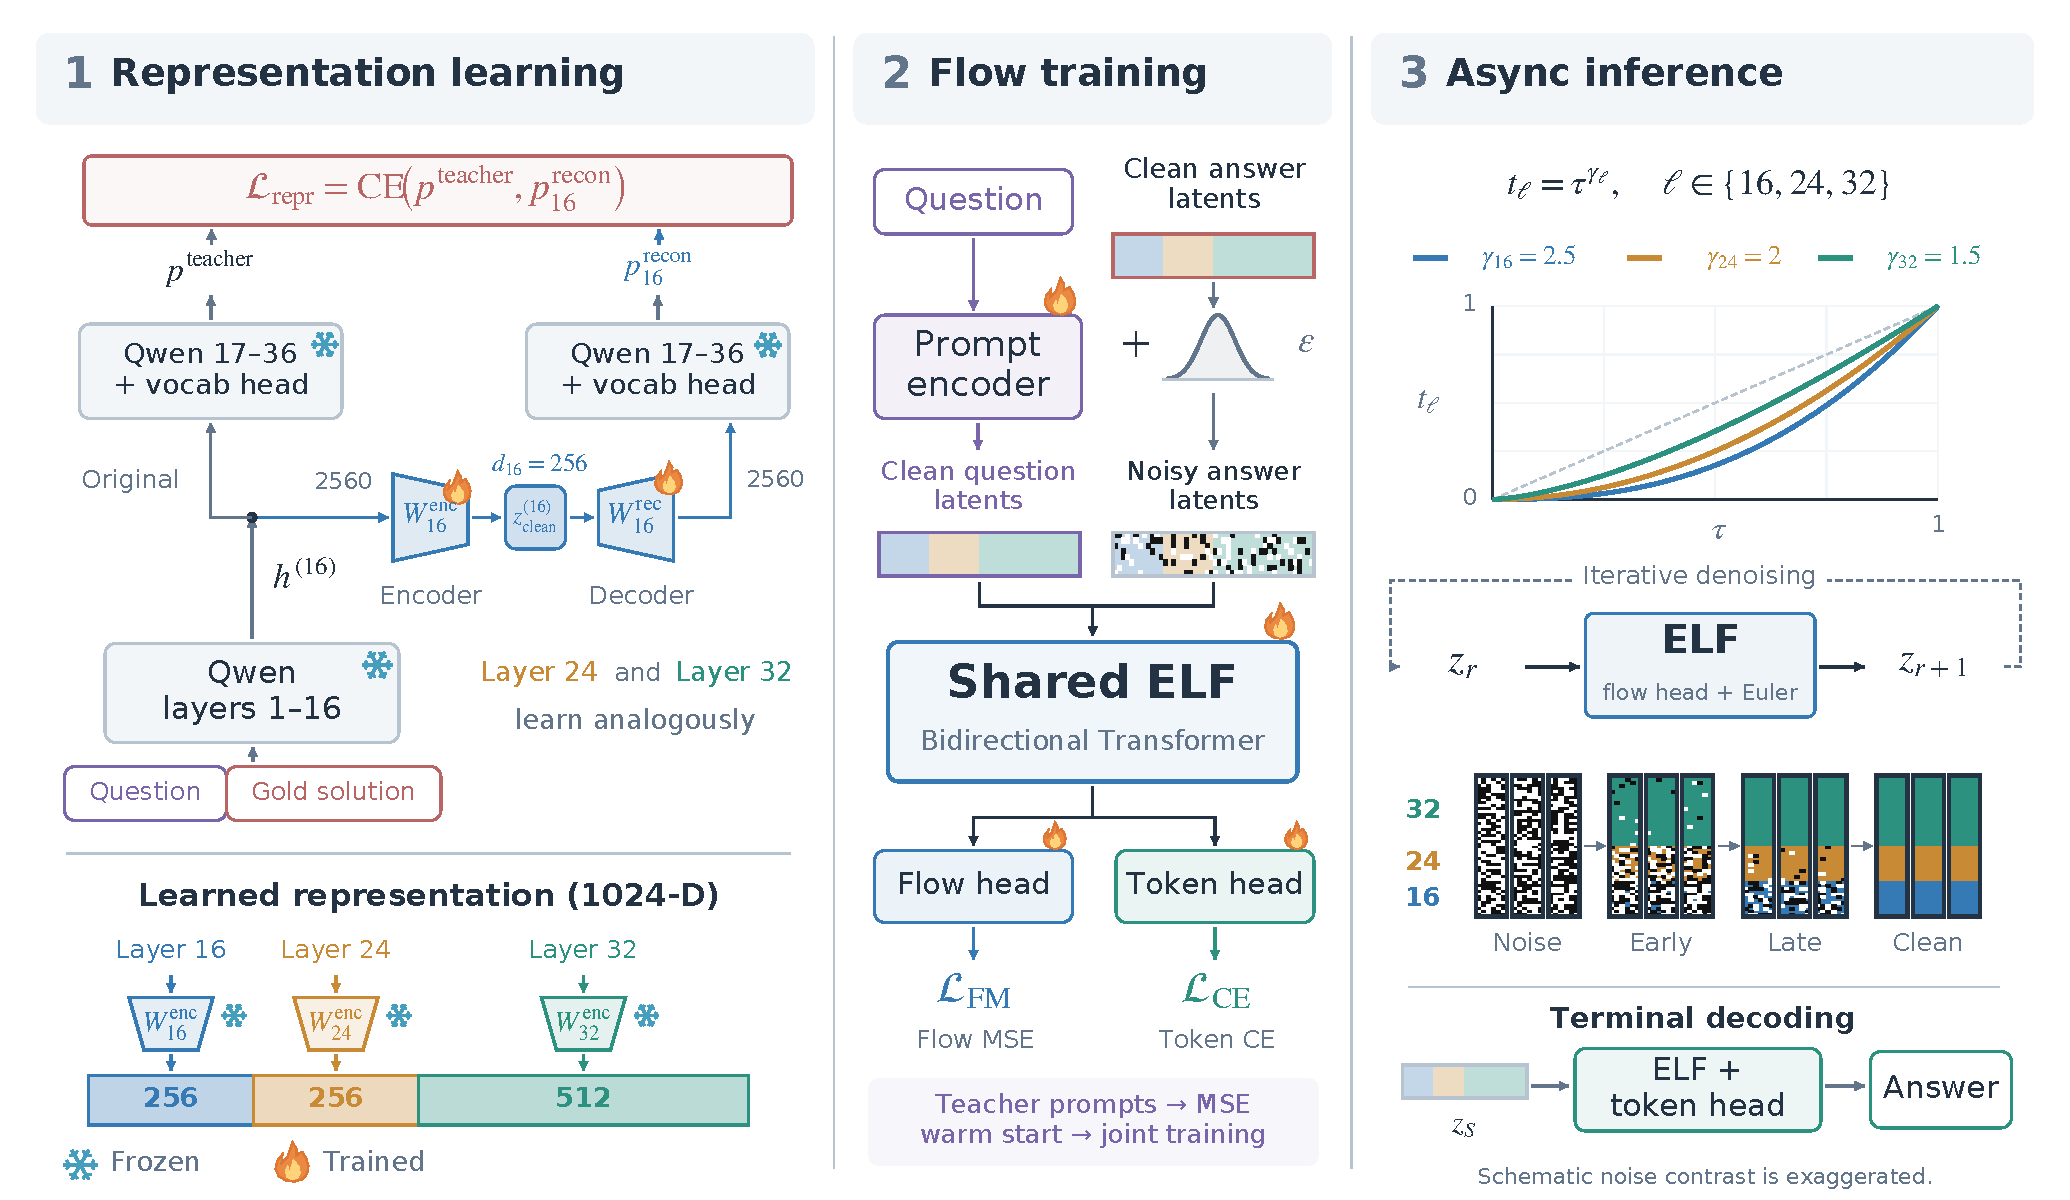
\includegraphics[width=\textwidth]{figures/pipeline_overview_v8.pdf}
    \caption{\textbf{The CEDR training and inference pipeline.}
    \textbf{Left:} Learn projections of Qwen layers 16/24/32 through teacher cross-entropy, then concatenate their outputs (Section~\ref{sec:representationconstruction}).
    \textbf{Center:} Train the ELF backbone with flow and token-decoding losses and staged prompt learning (Sections~\ref{sec:methodflow} and~\ref{sec:conditionalencoding}).
    \textbf{Right:} Denoise the representation groups under asynchronous clocks, then decode the answer in parallel (Section~\ref{sec:clocks}).}
    \label{fig:pipelineoverview}
\end{figure}

\textbf{Continuous denoising.}
ELF's bidirectional backbone predicts $\widehat z_{\mathrm{clean}}=F_\theta(z_t,t;c,\widehat z_{\mathrm{sc}},g)$ from the clean prompt and noisy answer at a shared training time $t$. Here $\widehat z_{\mathrm{sc}}$ is an earlier clean prediction and $g$ the guidance scale. We apply Eq.~\eqref{eq:basicflowloss} with velocity $v_\theta=(\widehat z_{\mathrm{clean}}-z_t)/\Delta_t$ and stabilized target $u_t^{\mathrm{stab}}=(z_{\mathrm{clean}}-z_t)/\Delta_t$, with $\Delta_t=\max(1-t,0.05)$; outside the clamp, $u_t^{\mathrm{stab}}=u_t$. Appendix~\ref{app:methodobjective} gives valid-token normalization.

\textbf{Self-conditioning and SCCFG.}
ELF's self-conditioning classifier-free guidance (SCCFG) learns to amplify answer self-conditioning at scale $g$. It compares predictions with and without \emph{answer self-conditioning}, retaining the prompt in both; Appendix~\ref{app:methodobjective} gives the detached guidance-adjusted target. Guidance is internal to the field, requiring one denoiser call per step.

\textbf{Recovering discrete tokens.}
A vocabulary head on the same backbone predicts same-position answer tokens under a separate decoder corruption $z^{\mathrm{dec}}$:
\begin{equation}
 \mathcal L_{\mathrm{CE}}
 =\E_{\mathrm{valid}}\!\left[-\log p_{\theta,j}^{\mathrm{tok}}(a_j\mid z^{\mathrm{dec}},c(q))\right].
 \label{eq:methoddecoderloss}
\end{equation}
The expectation averages valid answer tokens, including the terminal token; Appendix~\ref{app:methodobjective} specifies the exact batch weighting, decoder corruption, and mode mixing. At inference, encode the prompt once and keep it clean through $S$ Euler steps with recurrent self-conditioning; one additional backbone call decodes the answer in parallel and is excluded from denoising NFE.

\subsection{Learning the denoising representation}
\label{sec:representation}

The denoising representation must support generation and token recovery. We extract \textbf{teacher-forced Qwen3-4B-Instruct-2507 activations} \citep{qwen2507} in one forward pass; although these features are causal, our bidirectional denoiser jointly generates answer representations.

\textbf{Latent construction.}
\label{sec:representationconstruction}
Let $h_j^{(\ell)}$ be the frozen teacher's post-block activation at answer position $j$. We concatenate centered linear projections as $z_{\mathrm{clean},j}=\big[(h_j^{(\ell)}-\mu_\ell)W_\ell^{\mathrm{enc}}\big]_{\ell\in\mathcal S}$ for $\mathcal S=\{16,24,32\}$, with widths $(d_{16},d_{24},d_{32})=(256,256,512)$ and fixed means $\mu_\ell$. These maps initially also encode prompts; answer representations stay fixed during flow training and NFT.

\textbf{Learning the projectors.}
Linear decoders reconstruct $\widehat h_j^{(\ell)}=\mu_\ell+z_{\mathrm{clean},j}^{(\ell)}W_\ell^{\mathrm{rec}}$ (Figure~\ref{fig:pipelineoverview}, left). Replacing layer-$\ell$ answer activations with these reconstructions and running the frozen Qwen suffix yields next-token predictions $p_{\ell,j}^{\mathrm{recon}}$. We preserve the teacher's predictions through $\mathcal L_{\mathrm{repr}}=\sum_{\ell\in\mathcal S}\E_{q,a,j}\,\CE(p_j^{\mathrm{teacher}},p_{\ell,j}^{\mathrm{recon}})$, where $\CE$ is full-vocabulary soft cross-entropy. Only $W_\ell^{\mathrm{enc}}$ and $W_\ell^{\mathrm{rec}}$ are learned; the reconstruction decoders are used only at this stage. Appendix~\ref{app:representationimplementation} gives initialization, whitening, and scoring details.

\begin{figure}[tbp]
\centering
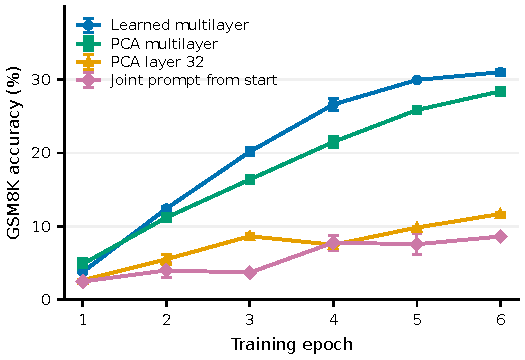
\includegraphics[width=.72\linewidth]{figures/representation_shared2_sd.pdf}
\caption{\textbf{Representation and conditioning affect reasoning.} CEDR-B learning curves on GSM8K, with ODE sampling, 32 steps, and $t=\tau^2$. The first three variants retain Qwen conditioning; the fourth jointly trains a randomly initialized prompt encoder. Protocol: Appendix~\ref{app:representationclock}; values and SDs: Table~\ref{tab:representationcurvevalues} (Appendix~\ref{app:representationclock}).}
\label{fig:representationcomparison}
\end{figure}

The first three arms in Figure~\ref{fig:representationcomparison} compare 1,024-dimensional whitened representations under matched six-epoch CEDR-B training and evaluation; Table~\ref{tab:representationcurvevalues} gives four-seed endpoint results.

\textbf{Decodability and representation choice.}
\label{sec:representationablations}
The fixed 1,024-dimensional layer-32 PCA representation supports \textbf{99.24\%} held-out same-position token recovery after two epochs of training a separate decoder (Appendix~\ref{app:representationdiagnostics}). Yet CEDR-B using this same representation achieves only \textbf{11.20\%} GSM8K accuracy after six epochs. Accurate clean-token recovery alone is therefore an insufficient criterion for choosing a denoising representation.

\textbf{Layer selection.}
We choose layers 16, 24, and 32 based on centered kernel alignment (CKA; \citealp{cka}) of Qwen activations (Figure~\ref{fig:representationcka}). The sharp transition after layer 16 motivates retaining that layer, followed by regularly spaced deeper features at layers 24 and 32. This is a motivation for the triplet, rather than an exhaustive search for optimal layers; Appendix~\ref{app:representationcka} gives the measurement protocol. Holding the projection method and total latent width fixed, multilayer PCA raises accuracy to \textbf{28.43\%} (Figure~\ref{fig:representationcomparison}). The resulting layer groups also enable distinct denoising clocks (Section~\ref{sec:clocks}).

\begin{figure}[htbp]
\centering
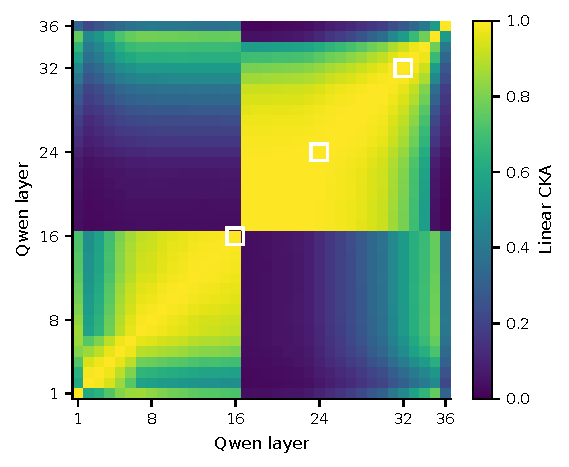
\includegraphics[width=.62\linewidth]{figures/cka.pdf}
\caption{\textbf{Qwen layer structure.} Linear CKA of teacher-forced activations on the combined discovery and confirmation panels. White markers select layers 16, 24, and 32. The transition after layer 16 motivates retaining that layer, followed by regularly spaced deeper features.}
\label{fig:representationcka}
\end{figure}

\textbf{Learned versus PCA.}
PCA preserves high-variance directions, which need not preserve the teacher's predictive behavior. Holding layers and latent widths fixed, learning the projectors through teacher cross-entropy raises accuracy from \textbf{28.43\% to 30.76\%} (Figure~\ref{fig:representationcomparison}).


\subsection{Learning the conditional encoding in three stages}
\label{sec:conditionalencoding}

ELF and ELF-REG use external contextual prompt encoders \citep{elf,scalingdlm}. We instead replace the Qwen teacher Transformer with a compact trainable encoder, retaining its frozen token lookup. For CEDR-L, the contextual network has \textbf{121M parameters}, compared with 3.63B in the full teacher Transformer (both excluding vocabulary input/output maps). The student uses six bidirectional attention blocks and encodes each prompt once; see Appendix~\ref{app:training} for its architecture.


\textbf{The prompt as the condition.}
The text-conditioned field $v_\Theta$ of Section~\ref{sec:preliminaries} includes self-conditioning and guidance as auxiliary inputs. We jointly optimize $\theta$ and $\phi$, keeping the prompt text, answer representation, and forward corruption fixed. The following lemma characterizes what the encoding must preserve.

\begin{lemma}[Preserving the text-conditional score]
\label{lem:conditionalrepresentation}
Let $Z_{\mathrm{clean}}$ and $Q$ denote the clean answer latents and prompt, with $\E\|Z_{\mathrm{clean}}\|_F^2<\infty$, and fix a deterministic encoder $C=P_\phi(Q)$. Let $s^\star(z,t\mid c)$ denote the score conditioned on $C=c$. Under the independent Gaussian corruption in Eq.~\eqref{eq:methodinterpolant}, for $0<t<1$ and $c=P_\phi(q)$,
\begingroup\small
\begin{equation}
 s^\star(z,t\mid q)-s^\star(z,t\mid c)
 =\frac{t}{\sigma^2(1-t)^2}
 \bigl(\E[Z_{\mathrm{clean}}\mid Z_t=z,Q=q]-\E[Z_{\mathrm{clean}}\mid Z_t=z,C=c]\bigr).
 \label{eq:conditionalscoredifference}
\end{equation}
\endgroup
Thus an encoder preserves the full-prompt score exactly when it preserves the posterior mean clean answer. If this holds along the path, the optimal unguided field also agrees by Eq.~\eqref{eq:conditionalflowscore}, giving the same conditional endpoint law under exact integration whenever the flow is well-defined.
\end{lemma}

\begin{figure}[tbp]
\centering
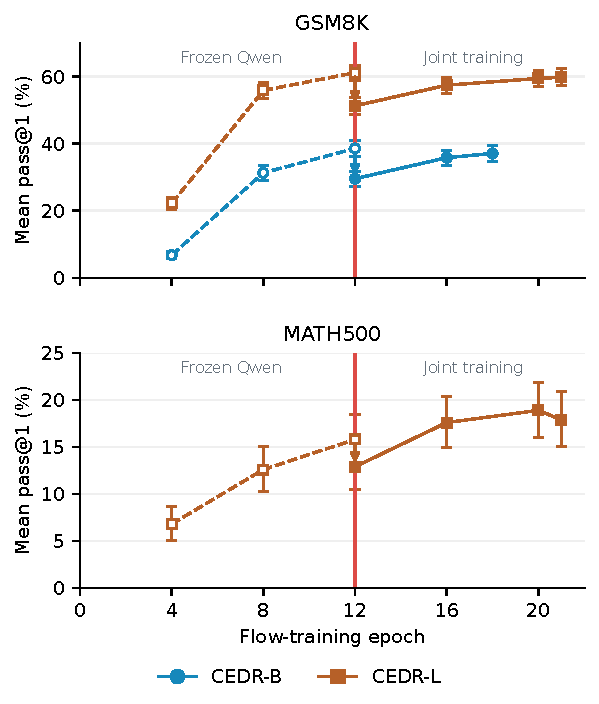
\includegraphics[width=.56\linewidth]{figures/prompt_curriculum_training_cedr_rerun.pdf}
\caption{\textbf{From teacher conditioning to learned prompts.} Top: GSM8K; bottom: MATH500. Circles/squares denote CEDR-B/L; open/filled markers denote Qwen/learned prompt encoding. Red line: epoch-12 switch; arrows: immediate MSE-swap loss. Values and settings: Appendix~\ref{app:promptcurves}.}
\label{fig:promptcurriculum}
\end{figure}

The encoder need not reproduce the teacher's coordinates: it must preserve the information needed for the posterior mean answer. Appendix~\ref{app:conditioninglemma} proves the lemma and gives an information-preserving encoding with arbitrarily large teacher-imitation MSE. MSE matching supplies a compatible initialization, while downstream training can adapt the encoder and denoiser jointly. We use three stages, keeping answer representations and token embeddings fixed throughout (details in Appendix~\ref{app:training}):

\textbf{1. Frozen conditioning.} Train the flow model for 12 epochs using fixed Qwen prompt representations and the flow/decoder objective. \textbf{2. Prompt imitation.} Freeze the flow model and fit the compact encoder to the teacher prompt representations using MSE. \textbf{3. Joint adaptation.} Substitute the learned encoder and optimize both networks through the flow/decoder objective, without an additional prompt-MSE loss, to epoch 18 for CEDR-B or epoch 21 for CEDR-L on the mathematical reasoning tasks.

Replacing Qwen with the MSE-trained encoder immediately reduces accuracy, despite unchanged flow-model weights (Figure~\ref{fig:promptcurriculum}). Subsequent joint training recovers much of this loss on GSM8K and exceeds the original teacher-conditioned checkpoint on MATH500. This recovery reflects adaptation of \emph{both} networks, showing the value of learning the conditioning interface through the generative objective.

\textbf{Importance of fixing initial conditioning.}
\label{sec:conditioningcurriculum}
Joint learning from initialization makes the conditioning interface change while the flow model is still learning to interpret it. Under the matched six-epoch comparison, this approach reaches only \textbf{8.70\%} GSM8K accuracy, versus \textbf{30.76\%} with frozen teacher conditioning (Figure~\ref{fig:representationcomparison}). This motivates stabilizing the condition during early learning and adapting it afterward.

Table~\ref{tab:trainingstages} summarizes the curriculum and reported NFT endpoints for each task. The coding joint stage additionally regularizes prompt features toward the teacher; Appendix~\ref{app:codingtraining} specifies this term.

\begin{table}[!htb]
\centering\small
\setlength{\tabcolsep}{5pt}
\caption{Training stages by task. Flow-training epochs count passes over answer rows; prompt-MSE epochs count passes over unique prompts and do not advance the flow-training epoch. Joint epochs are additional to the first 12 flow epochs. The last column gives the NFT checkpoint used for reporting, in successful optimizer updates, rather than a further epoch count.}
\label{tab:trainingstages}
\begin{tabular}{@{}lcccc@{}}
\toprule
Task / model & \shortstack{Frozen-Qwen\\flow epochs} & \shortstack{Prompt-MSE\\epochs} & \shortstack{Joint epochs\\(flow endpoint)} & \shortstack{Reported\\NFT update}\\
\midrule
GSM8K / CEDR-B & 12 & 60 & 6 (18) & 300\\
GSM8K / CEDR-L & 12 & 30 & 9 (21) & 600\\
MATH / CEDR-L & 12 & 10 & 9 (21) & 600\\
OpenCodeInstruct / CEDR-L & 12 & 10 & 1 (13) & 100\\
\bottomrule
\end{tabular}
\end{table}

\subsection{Asynchronous inference with local clocks}
\label{sec:clocks}

Our multilayer representation allows different feature groups to become clean at different rates, potentially letting one group use cleaner information from another. We extend the shared clock of Section~\ref{sec:preliminaries} to layer-specific clocks $t_\ell=f_\ell(\tau)=\tau^{\gamma_\ell}$ for $\ell\in\{16,24,32\}$ at inference, while retaining synchronous training. Equal exponents recover synchronous inference; unequal exponents give different noise levels within a single denoiser call.

\textbf{Adapting a synchronously trained denoiser.}
Although training uses a shared time, inference applies the same learned time-embedding function to each local time and averages its outputs, $\bar e_\theta^{\mathrm{time}}(\bm t)=\frac13\sum_\ell e_\theta^{\mathrm{time}}(t_\ell)$. This needs no retraining and recovers the original embedding when local times agree.


\textbf{Sampling with local clocks.}
Let $z_r$ be the answer state at solver time $\tau_r$, with local times $t_{\ell,r}=f_\ell(\tau_r)$, and let $\widehat z_{\mathrm{clean},r}$ denote the guided clean prediction. We use three sampling rules with the same trained denoiser and local clocks; the stochastic rules adapt established sampling procedures to the groupwise corruption in Eq.~\eqref{eq:methodinterpolant}.

\textbf{ODE.}
The Euler baseline advances the predicted velocity in the shared solver clock:
\begin{equation}
 z_{r+1}^{(\ell)}=z_r^{(\ell)}+
 (\tau_{r+1}-\tau_r)\,f'_\ell(\tau_r)
 \frac{\widehat z_{\mathrm{clean},r}^{(\ell)}-z_r^{(\ell)}}
 {\Delta_{t_{\ell,r}}},
 \label{eq:asyncsampler}
\end{equation}
where $\Delta_t=\max(1-t,0.05)$ is the stabilized denominator from Section~\ref{sec:methodflow}. No new noise is added after initialization.

\textbf{Stochastic (DMD2).}
Following the multistep sampling construction used in consistency models and DMD2 \citep{consistencymodels,dmd2}, predict the clean endpoint and apply fresh Gaussian corruption at the next local times:
\begin{equation}
 z_{r+1}^{(\ell)}
 =t_{\ell,r+1}\widehat z_{\mathrm{clean},r}^{(\ell)}
 +\sigma(1-t_{\ell,r+1})\xi_r^{(\ell)},
 \qquad \xi_r\sim\mathcal N(0,I).
 \label{eq:asyncdmd2}
\end{equation}
Noise is independent across steps and coordinates. We use this sampling construction without DMD2 distillation; ELF-REG also evaluates clean-prediction re-noising for continuous language generation \citep{scalingdlm}.

\textbf{Stochastic (EDM).}
Following EDM's noise-churn principle \citep{edm}, first move the current state to noisier local times $\bar t_{\ell,r}\leq t_{\ell,r}$. For an interior step, define $\alpha_{\ell,r}=\bar t_{\ell,r}/t_{\ell,r}$ and sample
\begin{equation}
 \bar z_r^{(\ell)}
 =\alpha_{\ell,r}z_r^{(\ell)}
 +\sigma\sqrt{(1-\bar t_{\ell,r})^2
 -\alpha_{\ell,r}^2(1-t_{\ell,r})^2}\,\xi_r^{(\ell)}.
 \label{eq:asyncchurnback}
\end{equation}
Evaluate the denoiser on $\bar z_r$ at $\bar{\bm t}_r$, giving a new clean prediction $\widehat z_{\mathrm{clean},r}$, then take an Euler step in each local time:
\begin{equation}
 z_{r+1}^{(\ell)}
 =\bar z_r^{(\ell)}
 +\frac{t_{\ell,r+1}-\bar t_{\ell,r}}{1-\bar t_{\ell,r}}
 \bigl(\widehat z_{\mathrm{clean},r}^{(\ell)}-\bar z_r^{(\ell)}\bigr).
 \label{eq:asyncchurnforward}
\end{equation}
This variant uses finite local-time increments and an Euler update, rather than EDM's original second-order solver. Appendix~\ref{app:samplerimplementation} specifies the churn times and endpoint rules.

All three samplers restore clean prompt positions and carry the guided clean prediction as recurrent self-conditioning. Each step uses one shared denoiser call for all groups, so asynchrony does not increase NFE; token decoding requires one additional call. Unlike shared-clock reparameterization, these local clocks expose the synchronously trained model to unequal group noise levels. The stochastic rules are discrete sampling procedures, without a claim that they integrate a particular continuous-time SDE.

\begin{table}[!htbp]
\centering\small
\setlength{\tabcolsep}{3pt}
\caption{\textbf{Inference-clock ablation across samplers.} CEDR-L epoch 21, 32 denoising steps, with headline guidance (SCCFG 2 for GSM8K, 3 for MATH500); mean pass@1 (\%) with seed SD over seeds 42/123. Bold marks the best clock within each dataset/sampler. EDM-style sampling uses index churn $0.7$; DMD2-style sampling uses $\eta=1$. Validation results, individual seeds, and paired comparisons appear in Appendix~\ref{app:schedulecomparisons}.}
\label{tab:inferenceclocks}
\begin{tabular}{@{}lrrrrrr@{}}
\toprule
& \multicolumn{2}{c}{ODE} & \multicolumn{2}{c}{Stochastic (EDM)} & \multicolumn{2}{c}{Stochastic (DMD2)} \\
\cmidrule(lr){2-3}\cmidrule(lr){4-5}\cmidrule(lr){6-7}
Clock powers & GSM8K & MATH500 & GSM8K & MATH500 & GSM8K & MATH500 \\
\midrule
$(1,1,1)$ & 52.62 {\scriptsize($\pm 0.75$)} & 16.70 {\scriptsize($\pm 0.42$)} & 59.78 {\scriptsize($\pm 0.05$)} & 19.60 {\scriptsize($\pm 1.70$)} & 60.50 {\scriptsize($\pm 0.43$)} & 21.10 {\scriptsize($\pm 2.69$)} \\
$(2,2,2)$ & 59.97 {\scriptsize($\pm 0.64$)} & 18.80 {\scriptsize($\pm 0.85$)} & 61.83 {\scriptsize($\pm 0.91$)} & 16.80 {\scriptsize($\pm 2.26$)} & 64.86 {\scriptsize($\pm 0.16$)} & 23.90 {\scriptsize($\pm 2.40$)} \\
$(1.5,2,2.5)$ & \textbf{60.08} {\scriptsize($\pm 0.38$)} & 18.50 {\scriptsize($\pm 0.14$)} & 63.42 {\scriptsize($\pm 0.59$)} & 19.90 {\scriptsize($\pm 0.99$)} & 66.49 {\scriptsize($\pm 0.86$)} & 25.00 {\scriptsize($\pm 2.55$)} \\
$(2.5,2,1.5)$ & 59.78 {\scriptsize($\pm 0.16$)} & \textbf{19.70} {\scriptsize($\pm 0.42$)} & \textbf{64.44} {\scriptsize($\pm 0.32$)} & \textbf{21.60} {\scriptsize($\pm 1.70$)} & \textbf{66.68} {\scriptsize($\pm 0.05$)} & \textbf{27.90} {\scriptsize($\pm 2.12$)} \\
\bottomrule
\end{tabular}
\end{table}

\textbf{Schedule choice and reasoning accuracy.}
Our headline results use $(\gamma_{16},\gamma_{24},\gamma_{32})=(2.5,2,1.5)$, chosen based on the highest observed MATH validation accuracy under ODE sampling; it also has the highest mean in the GSM8K ODE validation comparison (Appendix~\ref{app:schedulecomparisons}). Table~\ref{tab:inferenceclocks} compares the four clocks across all three samplers. With ODE, the nonidentity clocks improve on $(1,1,1)$, with small differences among them; forward asynchrony has the highest GSM8K mean and reverse asynchrony the highest MATH500 mean. Both stochastic samplers favor $(2.5,2,1.5)$ on both datasets. Under our DMD2-style headline sampler, this clock improves on $(2,2,2)$ by 1.82 percentage points on GSM8K and 4.00 on MATH500. The two asynchronous clocks remain close on GSM8K, whereas the reverse clock leads by 2.90 points on MATH500. Appendix~\ref{app:schedulecomparisons} gives paired uncertainty. These results support the chosen schedule without establishing a universally optimal clock; we keep it fixed across headline samplers and checkpoints.

Reconstruction probes reveal distinct sensitivities across layer groups, with weaker contrasts under random coordinate grouping (Figure~\ref{fig:layerreconstruction}). These findings motivate studying coordinated denoising across representations, but do not establish the mechanism behind the sampling gains.

% END continuous diffusion framework and design choices

\section{Reinforcement learning with self-conditioned flows}
\label{sec:nft}

DiffusionNFT \citep{diffusionnft} improves continuous generators through rewarded endpoint regression, without differentiating through sampling trajectories. We adapt it to CEDR's learned self-conditioning guidance and supplement sparse correctness rewards with gold-solution endpoints.

\subsection{NFT with learned self-conditioning guidance}
\label{sec:nftsccfg}

\textbf{The velocity field optimized by standard NFT.}
Let $v_{\mathrm{cur}}$ and $v_{\mathrm{old}}$ denote the current and old policy velocity fields, $u$ a sample's forward velocity target, and $\rho\in[0,1]$ its normalized optimality coefficient. NFT forms implicit positive and negative velocity fields, $v^+=(1-\beta)v_{\mathrm{old}}+\beta v_{\mathrm{cur}}$ and $v^-=(1+\beta)v_{\mathrm{old}}-\beta v_{\mathrm{cur}}$. For current and old velocity-field values $f,h$, the pointwise loss is
\begin{equation}
 \ell_\beta(f,h;u,\rho)
 =\rho\|(1-\beta)h+\beta f-u\|_2^2
 +(1-\rho)\|(1+\beta)h-\beta f-u\|_2^2.
\label{eq:nftquadratic}
\end{equation}
Standard NFT applies this loss to $f=v_{\mathrm{cur}}$ and $h=v_{\mathrm{old}}$, holding the old field fixed; its original experiments use CFG-free optimization \citep{diffusionnft}. CEDR instead learns a guidance-conditioned field, motivating a correction before applying NFT's regression objective.

\textbf{Constructing the SCCFG-compatible field.}
For each policy $p\in\{\mathrm{cur},\mathrm{old},\mathrm{ref}\}$, forward-noise an endpoint and obtain velocity $v_p^0$ from a detached bootstrap without answer self-conditioning. The main prediction $v_p^{\mathrm{main}}$ uses the bootstrap clean endpoint when $b_{\mathrm{sc}}=1$ and zero answer self-conditioning otherwise; both passes retain the question. Following ELF's guidance construction, define
\begin{equation}
 \widetilde v_p=v_p^{\mathrm{main}}-
 \sg\!\left[b_{\mathrm{sc}}(1-g^{-1})(v_p^{\mathrm{main}}-v_p^0)\right],
 \label{eq:nftcorrectedfield}
\end{equation}
where $g>0$ is the SCCFG scale. Our update applies Eq.~\eqref{eq:nftquadratic} to $f=\widetilde v_{\mathrm{cur}}$, $h=\sg(\widetilde v_{\mathrm{old}})$, and $u=u_t^{\mathrm{stab}}$ from Section~\ref{sec:methodflow}. We use $\beta=1$ and add a squared-velocity penalty toward the corrected field $\widetilde v_{\mathrm{ref}}$ of the fixed initial reference. With self-conditioning enabled, the corrected value is $v_p^0+(v_p^{\mathrm{main}}-v_p^0)/g$. Detaching the correction preserves the main-pass Jacobian rather than scaling it by $1/g$ (Appendix~\ref{app:nftdetails}).

\textbf{Guided rollouts and forward-process updates.}
Collection retains recurrent self-conditioning and SCCFG guidance. We reward decoded answers but optimize their saved continuous endpoints, using fresh forward corruption and bootstrap predictions rather than replaying rollout histories. Thus rollouts remain guided while NFT optimizes the corrected fields in Eq.~\eqref{eq:nftcorrectedfield}.

\subsection{Gold-anchored reasoning updates}
\label{sec:nftgold}

Each question contributes 15 old-policy generations and one gold latent endpoint, with raw rewards 0.75 for correct generated answers, 0 for incorrect answers, and 1 for gold. The gold endpoint supplies a preferred target even when all generated answers are incorrect. We discard groups whose generated answers are all correct, concentrating updates on observed failures; retained rewards are normalized into $\rho$ as described in Appendix~\ref{app:nftdetails}. This recipe uses reference solutions as well as verifiable rewards. Gold raw reward one need not give $\rho_G=1$; the following lemma characterizes its contribution.

\begin{lemma}[Gold endpoints as field anchors]
\label{lem:goldanchor}
For a gold endpoint, let $\mathcal H$ contain the noisy state, time, question, coefficient $\rho_G\in[1/2,1]$, and any auxiliary inputs held fixed for the update. Let $U$ denote the random stabilized target $u_t^{\mathrm{stab}}$, assume its conditional second moment is finite, and set $m_G=\E[U\mid\mathcal H,\mathrm{gold}]$. For $\mathcal H$-measurable current and old velocity-field values $f,h$, define $a_G=(2\rho_G-1)m_G+2(1-\rho_G)h$. The beta-one NFT loss satisfies
\begin{equation}
 \E[\ell_1(f,h;U,\rho_G)\mid\mathcal H,\mathrm{gold}]
 =\|f-a_G\|_2^2+C_{\mathcal H},
\label{eq:nftgoldanchor}
\end{equation}
where $C_{\mathcal H}$ is independent of $f$ with the conditioning information and auxiliary fields fixed. Thus the gold term attracts the current field toward a convex combination of the gold posterior target and the old field.
\end{lemma}

At $\rho_G=1$, the gold term directly regresses toward $m_G$. Under an ideal reference model matching that gold posterior target, the anchor interpolates between the reference and old fields; Appendix~\ref{app:nftgoldproof} gives the proof and scope. This gold-induced anchor complements the explicit reference penalty.

Because the external condition is the question text, NFT jointly updates the prompt encoder and flow model as one conditional policy (Lemma~\ref{lem:conditionalrepresentation}), without a prompt-imitation objective. Training uses synchronous identity clocks; asynchronous evaluation follows Section~\ref{sec:clocks}. Appendix~\ref{app:training} gives optimization details, and Sections~\ref{sec:nftresults} and~\ref{sec:codingresults} discuss the empirical gains.

\section{Empirical Evaluation}
\label{sec:headlineresults}

We evaluate mathematical reasoning on GSM8K and MATH500 \citep{gsm8k,math,math500}, and code generation in Section~\ref{sec:codingresults}. Math evaluations use zero-shot prompts, async clocks $(2.5,2,1.5)$, numerical-answer scoring for GSM8K, and Math-Verify for MATH500 \citep{mathverify}. All CEDR headline results use the same DMD2-style stochastic sampler (Eq.~\eqref{eq:asyncdmd2}, noise multiplier $\eta=1$) across checkpoints, datasets, and NFEs. Math headline pass@1 averages eight sampling seeds at 64 denoising steps. Representation and prompt-learning ablations retain ODE sampling; the schedule ablation compares all three samplers. NFE counts denoising calls, excluding prompt encoding and terminal decoding. Appendices~\ref{app:experimentdetails} and~\ref{app:seedvariability} give checkpoint settings and seed standard deviations.

\subsection{Mathematical reasoning}
\label{sec:mathresults}
\begin{table}[!htb]
\caption{Mathematical reasoning across model families, mean pass@1 (\%). Parameters are in millions (three significant digits). Embedding Params count vocabulary input/output maps, tied weights once; Other Params count remaining weights, with $(+X)$ used once per response. Frozen components are included. $^{*}N$ denotes $N-1$ denoising calls for ELF-REG. Bold/underline mark first/second within each sub-billion continuous-backbone group.}
\label{tab:headlinecomparison}
\centering\small
\setlength{\tabcolsep}{4pt}
\begin{tabular}{@{}lrrrrr@{}}
\toprule
Model & \shortstack{Embedding\\Params (M)} & \shortstack{Other\\Params (M)} & NFE & GSM8K & MATH500\\
\midrule
\multicolumn{6}{@{}l}{\textit{Autoregressive}}\\
Qwen3-0.6B-Base \citep{qwen3} & 156 & 440 & --- & 59.59 & ---\\
Qwen3-0.6B, thinking \citep{qwen3} & 156 & 440 & --- & --- & 77.60\\
\midrule
\multicolumn{6}{@{}l}{\textit{Discrete diffusion / blockwise diffusion}}\\
LLaDA-8B-Base \citep{llada} & 1,040 & 6,980 & 1,024 & 70.30 & ---\\
Dream-v0-Base-7B \citep{dream} & 1,090 & 6,530 & 256 & 77.20 & ---\\
SDAR-1.7B-Chat \citep{sdar} & 622 & 1,410 & 4/block & 80.10 & 63.20\\
\midrule
\multicolumn{6}{@{}l}{\textit{Continuous diffusion / flow: denoising backbone below 200M}}\\
\shortstack[l]{$\mathbb S$-FLM (top-1)\\\citep{hyperspherical}} & 75.5 & 87.5 & 1,024 & 18.00$^\dagger$ & ---\\
FMLM+ Init \citep{posterior} & 75.5 & 92 & 64 & 33.60$^\dagger$ & ---\\
ELF-REG-B (stoch.) \citep{scalingdlm} & 311 & 104 $(+441)$ & $^{*}64$ & 42.97 & ---\\
\textbf{CEDR-B, pre-NFT (ours)} & 545 & 90.4 $(+45.8)$ & 64 & \textbf{47.62} & ---\\
\textbf{CEDR-B, post-NFT (ours)} & 545 & 90.4 $(+45.8)$ & 64 & \underline{47.00} & ---\\
\midrule
\multicolumn{6}{@{}l}{\textit{Continuous diffusion / flow: denoising backbone 200M--1B}}\\
ELF-REG-L (stoch.) \citep{scalingdlm} & 311 & 652 $(+442)$ & $^{*}64$ / $^{*}128$ & 61.28 & 20.15\\
\textbf{CEDR-L, pre-NFT (ours)} & 545 & 638 $(+123)$ & 64 & \underline{67.13} & \underline{28.58}\\
\textbf{CEDR-L, post-NFT (ours)} & 545 & 638 $(+123)$ & 64 & \textbf{68.97} & \textbf{32.40}\\
\midrule
\multicolumn{6}{@{}l}{\textit{Continuous diffusion / flow: larger backbones (reference)}}\\
MLFM \citep{mlfm} & 123 & 1,220 & NR$^\S$ & 31.24 & ---\\
TESS 2, GSM8K FT \citep{tess2} & 262 & 6,740 & 1,000 & $\approx68.9^\ddagger$ & ---\\
\bottomrule
\end{tabular}
\vspace{3pt}
\parbox{\linewidth}{\footnotesize External results are author-reported. ELF-REG uses its best reported stochastic settings (v3, Tables 4 and 30); CEDR uses DMD2-style sampling throughout. Table~\ref{tab:elfregselected} records the selected ELF-REG settings and seed SDs. $^\dagger$Python scoring, $^\ddagger$Approximate accuracy read from TESS 2 Figure 3b. $^\S$MLFM reports 256 sampling steps with guidance and online token promotion; the corresponding NFE is not established (NR). Slashes separate GSM8K/MATH500 budgets. Appendix~\ref{app:experimentdetails} details prompting and parameter accounting; Table~\ref{tab:headlineseedsd} in Appendix~\ref{app:seedvariability} gives our seed SDs.}
\end{table}

\textbf{Reasoning accuracy across denoising budgets.}
\label{sec:headlinecomparison}
\label{sec:headlinelownfe}
At comparable denoising-backbone sizes, both supervised and post-NFT CEDR exceed the reported continuous-diffusion baselines at the headline budgets (Table~\ref{tab:headlinecomparison}). Supervised CEDR-L reaches 67.13\% on GSM8K and 28.58\% on MATH500, versus ELF-REG-L's strongest reported 61.28\% and 20.15\%; post-NFT CEDR-L reaches 68.97\% and 32.40\%. CEDR-B reaches 47.62\% before NFT and 47.00\% afterward, both above ELF-REG-B's 42.97\%. Our 90.4M/638M denoisers use compact learned prompt encoders, without executing the teacher Transformer during generation. The autoregressive, discrete-diffusion, and larger continuous-model rows provide broader context; training data, scale, and evaluation protocols differ.

\begin{table}[!htb]
\caption{Reasoning at lower NFE, mean pass@1 (\%). Table~\ref{tab:headlinecomparison} gives model parameter counts. Bold/underline mark first/second within each benchmark and backbone-scale block; $^{*}$ marks one fewer denoising call than the heading. External results follow \citet{posterior,scalingdlm}; Appendix~\ref{app:experimentdetails} gives source and protocol details.}
\label{tab:headlinelownfe}
\centering\small
\setlength{\tabcolsep}{1.7pt}
\begin{tabular}{@{}l*{12}{r}@{}}
\toprule
& \multicolumn{4}{c}{GSM8K ($\sim$100M)} & \multicolumn{4}{c}{GSM8K ($\sim$650M)} & \multicolumn{4}{c}{MATH500 ($\sim$650M)}\\
\cmidrule(lr){2-5}\cmidrule(lr){6-9}\cmidrule(lr){10-13}
Method / NFE & 8 & 16 & 32 & 64 & 8 & 16 & 32 & 64 & 8 & 16 & 32 & 64\\
\midrule
FMLM+ Init & 15.10 & 26.10 & 31.80 & 33.60 & --- & --- & --- & --- & --- & --- & --- & ---\\
ELF-REG (best) & $^{*}$\underline{26.88} & $^{*}$\underline{38.53} & $^{*}$41.17 & $^{*}$42.97 & $^{*}$48.69 & $^{*}$56.90 & $^{*}$59.95 & $^{*}$61.28 & $^{*}$9.85$^{\dagger}$ & $^{*}$14.00 & $^{*}$17.25 & $^{*}$20.00\\
CEDR, pre-NFT & 24.95 & 38.25 & \underline{44.39} & \textbf{47.62} & \underline{54.23} & \underline{62.57} & \underline{65.71} & \underline{67.13} & \underline{16.70} & \underline{21.75} & \underline{25.76} & \underline{28.58}\\
CEDR, post-NFT & \textbf{28.48} & \textbf{40.60} & \textbf{45.59} & \underline{47.00} & \textbf{57.93} & \textbf{64.96} & \textbf{67.59} & \textbf{68.97} & \textbf{18.82} & \textbf{25.26} & \textbf{29.80} & \textbf{32.40}\\
\bottomrule
\end{tabular}
\vspace{3pt}
\parbox{\linewidth}{\footnotesize CEDR uses DMD2-style sampling and fixed checkpoints, with SCCFG 2 for GSM8K and 3 for MATH500. ELF-REG reports four-seed means: stochastic sampling except $^\dagger$ODE; settings can differ across budgets (Table~\ref{tab:elfregselected}). Our sampling-seed counts and SDs: Table~\ref{tab:headlineseedsd} in Appendix~\ref{app:seedvariability}.}
\end{table}

Supervised CEDR-L exceeds the reported comparable-scale baselines on both GSM8K and MATH500 at every displayed budget (Table~\ref{tab:headlinelownfe}). Supervised CEDR-B exceeds ELF-REG-B at 32 and 64 calls but trails it in the two smaller-budget comparisons; post-NFT CEDR-B exceeds it at all four budgets. Useful reasoning emerges without training a separate few-step student. These are reported operating points with different training and evaluation protocols; NFE does not equate FLOPs across methods. Both headline tables and inference-allocation curves use SCCFG 2 for GSM8K and 3 for MATH500.

\textbf{Refining an answer or drawing more answers.}
\label{sec:headlinebudget}
For $k$ samples with $S$ denoising steps each, we use $kS$ as the inference budget. Oracle pass@$k$ measures whether any sample is correct; majority vote selects the most frequent final answer after grouping equivalent answers, without consulting the reference. For selectors returning one of the generated answers, voting provides an achievable \emph{lower bound} on optimal selection accuracy, while oracle pass@$k$ supplies its \emph{upper bound}. We compare $S\in\{8,16,32,64\}$ up to a budget of 512 calls; Appendix~\ref{app:budgetvalues} gives aggregation details.

\begin{figure}[!htbp]
\centering
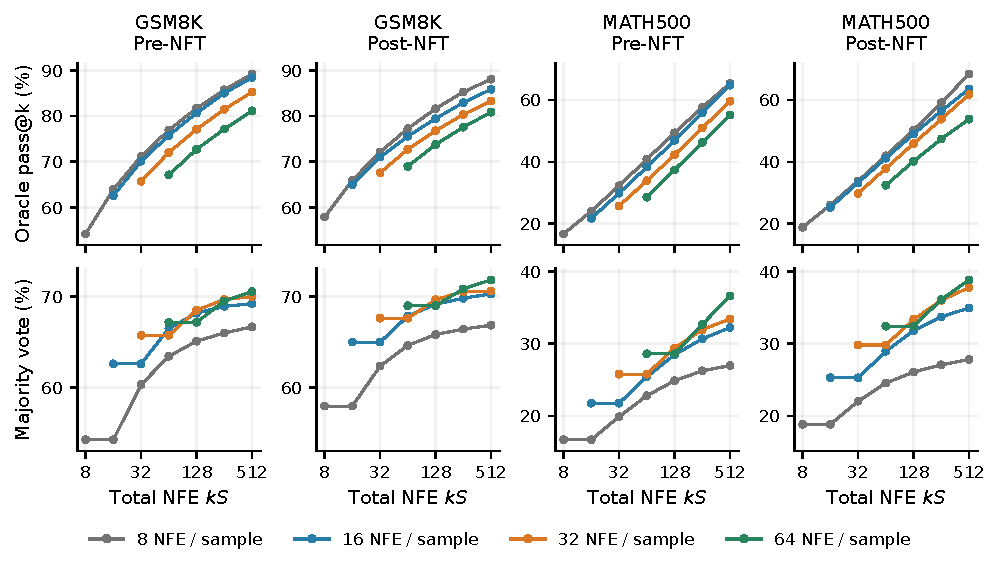
\includegraphics[width=\linewidth]{figures/headline_stages_dmd2.pdf}
\caption{CEDR-L before and after NFT with DMD2-style sampling: GSM8K uses SCCFG 2 and MATH500 uses SCCFG 3. Top: oracle pass@$k$; bottom: majority-vote accuracy. Colors denote denoising NFE per sample; the budget is $kS$. Numerical values appear in Appendix~\ref{app:budgetvalues}; Appendix~\ref{app:elfbbudgets} gives the corresponding CEDR-B curves.}
\label{fig:headlinestages}
\end{figure}

Figure~\ref{fig:headlinestages} shows that oracle selection generally favors more attempts with fewer steps, whereas voting generally favors higher-NFE samples. On MATH500 after NFT, 64 eight-step samples reach 68.40\% oracle accuracy, versus 53.80\% for eight 64-step samples; voting reverses this preference, at 27.80\% versus 38.80\%. Intermediate depths remain competitive for voting. The voting--oracle gap motivates better answer selection, potentially using latent-space or hidden-state classifiers.

The corresponding GSM8K CEDR-B comparison appears in Appendix~\ref{app:elfbbudgets}. Appendix~\ref{app:samplerallocations} compares these allocations across ODE and both stochastic samplers.

\textbf{What changes after NFT?}
\label{sec:nftresults}
Under DMD2-style sampling, NFT improves CEDR-L pass@1 at all four denoising depths: the 64-step gains are $+1.84$ percentage points on GSM8K and $+3.83$ on MATH500. The effect is not uniform across models and metrics. CEDR-B improves at 8--32 calls but changes from 47.62\% to 47.00\% at 64 calls. High-$k$ oracle coverage can also decrease: with eight 64-step samples, MATH500 pass@8 changes from 55.20\% to 53.80\%, while voting improves from 36.58\% to 38.80\%. At eight steps and 64 samples, MATH500 oracle accuracy instead rises from 65.40\% to 68.40\%. Voting depends on the correct answer's frequency relative to competing answers, whereas oracle selection needs only one successful draw. These patterns show that NFT gains depend on the inference allocation; they do not establish a loss of reasoning diversity. Appendix~\ref{app:budgetvalues} gives paired uncertainty, and Appendices~\ref{app:generations}--\ref{app:trajectories} illustrate ODE generations.

\paragraph{Higher-pass comparison with continuous-diffusion baselines.}
At 64 denoising calls, supervised and post-NFT CEDR-L with DMD2-style sampling reach MATH500 pass@8 of 55.20\% and 53.80\%. Both exceed ELF-REG-L's reported ODE pass@10 of 44.04\% at 63 denoising calls (Table~\ref{tab:mathhigherpass}; \citealp[v3, Table 20]{scalingdlm}). This compares different attempt counts, not equal compute or an estimate of our pass@10. CEDR uses SCCFG 3 throughout these headline comparisons.

\begin{table}[!htbp]
\centering\small
\setlength{\tabcolsep}{8pt}
\caption{\textbf{MATH500 oracle accuracy at higher sample counts.} CEDR-L uses learned prompt conditioning, SCCFG 3, and eight saved draws. ELF-REG-L retains its external prompt encoder. CEDR uses DMD2-style sampling and ELF-REG uses ODE; ELF-REG's stochastic study reports only four draws and cannot supply pass@8/10. NFE counts denoising calls per sample; $k\times\mathrm{NFE}$ makes the differing total budgets explicit. These are cross-paper reported results, with protocol details in Appendix~\ref{app:experimentdetails}. Table~\ref{tab:budgetvaluesmathl} gives our uncertainty estimates.}
\label{tab:mathhigherpass}
\begin{tabular}{@{}lrrrr@{}}
\toprule
Model & NFE & $k$ & $k\times\mathrm{NFE}$ & Pass@$k$ (\%)\\
\midrule
ELF-REG-L \citep{scalingdlm} & 63 & 8 & 504 & 40.41\\
ELF-REG-L \citep{scalingdlm} & 63 & 10 & 630 & 44.04\\
CEDR-L, pre-NFT & 64 & 8 & 512 & 55.20\\
CEDR-L, post-NFT & 64 & 8 & 512 & 53.80\\
\bottomrule
\end{tabular}
\end{table}

\FloatBarrier
\subsection{Code generation}
\label{sec:codingresults}

On OpenCodeInstruct \citep{opencodeinstruct}, CEDR-L uses 12 epochs of frozen-Qwen flow training, ten prompt-MSE epochs, one joint epoch, and 100 NFT updates with execution-based rewards (Appendix~\ref{app:training}). Our rows in Table~\ref{tab:codingcomparison} use DMD2-style sampling, eight seeds, 128 denoising calls, async $(2.5,2,1.5)$, and SCCFG 3.

\begin{table}[!htbp]
\centering\small
\setlength{\tabcolsep}{5pt}
\caption{\textbf{Code generation under separate scoring conventions.} Mean pass@1 (\%). HE/HE+ use base/full extended tests; both MBPP columns use 378 tasks. PlaidQ's ``MBPP+'' uses base tests. CEDR uses DMD2-style sampling and eight seeds; pre-NFT is joint epoch 13 and post-NFT is update 100. ODE stage comparisons appear in Appendix~\ref{app:codingdetails}. ELF-REG uses ODE with 16 seeds in the standard block and its stronger stochastic sampler with four seeds in the alias block (v3, Tables 15 and 4). $^{*}128$ denotes 127 denoising calls for ELF-REG; all budgets exclude terminal decoding. The alias block allows single-function entry-point repair; rows across blocks should not be ranked together. Appendix~\ref{app:codingdetails} gives remaining protocol differences and seed SDs.}
\label{tab:codingcomparison}
\begin{tabular}{@{}lrrrrr@{}}
\toprule
Model / setting & \shortstack{Denoising\\NFE} & HE & HE+ & \shortstack{MBPP-378\\base} & \shortstack{MBPP+\\full}\\
\midrule
\multicolumn{6}{@{}l}{\textit{Standard scoring: no function-name repair}}\\
PlaidQ \citep{plaidq} & 128 & 19.02 & 18.05 & 22.18 & ---\\
PlaidQ+CFG \citep{plaidq} & 256 & 22.04 & 19.70 & 24.58 & ---\\
ELF-REG-L (ODE) \citep{scalingdlm} & $^{*}128$ & 22.26 & 21.15 & 24.21 & ---\\
\addlinespace
CEDR-L, pre-NFT (ours) & 128 & 39.71 & 35.75 & 28.08 & 24.34\\
CEDR-L, post-NFT (ours) & 128 & 40.09 & 36.74 & 27.94 & 24.83\\
\midrule
\multicolumn{6}{@{}l}{\textit{Single-function name aliasing}}\\
ELF-REG-L (stoch.) \citep{scalingdlm} & $^{*}128$ & 33.08 & 31.40 & 38.76 & ---\\
CEDR-L, pre-NFT (ours) & 128 & 39.94 & 35.82 & 45.01 & 38.72\\
CEDR-L, post-NFT (ours) & 128 & 40.63 & 36.89 & 45.63 & 39.48\\
\bottomrule
\end{tabular}
\end{table}

Under standard scoring, both supervised and post-NFT CEDR exceed reported PlaidQ and ELF-REG results on HumanEval(+), and exceed guided PlaidQ on MBPP-378 base. Under function-name aliasing, both exceed ELF-REG-L's strongest reported stochastic results on all three available metrics (Table~\ref{tab:codingcomparison}). Prompts and execution limits still differ across papers (Appendix~\ref{app:codingdetails}). With DMD2-style sampling, additional NFT gains are modest: standard pass@1 changes by $+0.38$ points on HumanEval, $+0.99$ on HumanEval+, $-0.13$ on MBPP-378 base, and $+0.50$ on MBPP+. All four paired 95\% intervals include zero (Table~\ref{tab:codingsdedeltas}). Thus the strong coding results primarily reflect the supervised model and sampler; this short NFT run provides weaker evidence of additional improvement.

\paragraph{Prompt adaptation remains task dependent.}
In the ODE stage ablation, with identical epoch-12 flow weights and 32 denoising steps, replacing Qwen with the encoder after one MSE epoch reduces HumanEval+ from 25.61\% to 18.60\% and MBPP+ from 32.34\% to 7.61\% (Table~\ref{tab:codingstages}). Ten MSE epochs recover HumanEval+ to 24.70\%, close to teacher conditioning, but MBPP+ reaches only 15.15\%. The 24.74-point initial MBPP+ drop is substantially larger than the prompt-swap losses in mathematical reasoning (Figure~\ref{fig:promptcurriculum}). These comparisons use the respective tasks' selected prompt checkpoints, rather than equal imitation-training budgets.

This replaces a 3.63B-parameter contextual teacher with a 121M-parameter prompt encoder, excluding vocabulary maps. Unique formatted training prompts average 233.44 tokens for code, versus 84.17 for GSM8K and 89.15 for MATH; longer contexts may make the compression harder, although we have not isolated length as the cause. With ODE at 128 steps, one joint epoch improves HumanEval(+) pass@1 by 1.60 points but decreases standard MBPP-378 base/MBPP+ by 1.16/0.56 points; subsequent NFT improves all four metrics. The conditioning interface therefore remains a meaningful design challenge. ELF-REG retains an approximately 440M-parameter contextual encoder, while our frozen-Qwen reference uses a much larger teacher, so neither comparison isolates encoder capacity. Appendix~\ref{app:codingdetails} gives the full trajectories, prompt-length statistics, and paired comparisons.

\paragraph{Higher-pass code generation.}
The eight saved draws also support oracle pass@8 (Table~\ref{tab:codinghigherpass}). Without function-name repair, pre- and post-NFT CEDR-L exceed PlaidQ+CFG's reported pass@10 on HumanEval and HumanEval+. Under aliasing, both exceed ELF-REG-L's reported ODE pass@8 and pass@10 on all three metrics. Its stochastic study provides only four draws, so this higher-pass comparison does not include that sampler. The higher-pass comparison on standard MBPP-378 remains weaker: our post-NFT pass@8 is 42.59\%, compared with guided PlaidQ's pass@10 of 44.79\%. These comparisons retain each paper's attempt count and scoring category; we do not infer CEDR pass@10 from eight draws. Tables~\ref{tab:codingstandarddetail}--\ref{tab:codingaliasdetail} give pass@1/2/4/8 and uncertainty for every CEDR stage.

\begin{table}[!htbp]
\centering\small
\setlength{\tabcolsep}{4.5pt}
\caption{\textbf{Oracle code accuracy with multiple attempts.} Entries are pass@$k$ (\%) at the stated $k$, with denoising NFE per sample. Our learned-conditioning rows use eight draws; external pass@10 values remain labeled as such. PlaidQ uses token-prefix conditioning and ELF-REG-L an external contextual encoder. Separate blocks retain standard versus alias scoring, and both MBPP columns use the same 378 tasks. External values are from PlaidQ Table 1 and ELF-REG v3 Table 18. CEDR uses DMD2-style sampling and ELF-REG uses ODE; ELF-REG does not report stochastic pass@8/10. Generation protocols and total compute differ.}
\label{tab:codinghigherpass}
\begin{tabular}{@{}lrrrrrr@{}}
\toprule
Model & NFE & $k$ & HE & HE+ & \shortstack{MBPP-378\\base} & \shortstack{MBPP+\\full}\\
\midrule
\multicolumn{7}{@{}l}{\textit{Standard scoring: no function-name repair}}\\
PlaidQ \citep{plaidq} & 128 & 10 & 25.72 & 24.03 & 34.33 & ---\\
PlaidQ+CFG \citep{plaidq} & 256 & 10 & 39.87 & 36.74 & 44.79 & ---\\
CEDR-L, pre-NFT & 128 & 8 & 56.71 & 53.66 & 44.71 & 38.36\\
CEDR-L, post-NFT & 128 & 8 & 58.54 & 53.66 & 42.59 & 37.83\\
\midrule
\multicolumn{7}{@{}l}{\textit{Single-function name aliasing}}\\
ELF-REG-L \citep{scalingdlm} & 127 & 8 & 46.42 & 44.22 & 52.89 & ---\\
ELF-REG-L \citep{scalingdlm} & 127 & 10 & 48.87 & 46.69 & 55.05 & ---\\
CEDR-L, pre-NFT & 128 & 8 & 57.32 & 53.66 & 60.58 & 51.59\\
CEDR-L, post-NFT & 128 & 8 & 59.15 & 54.27 & 59.52 & 50.53\\
\bottomrule
\end{tabular}
\end{table}


\section{Discussion and Conclusion}
\label{sec:conclusion}

CEDR shows that continuous latent diffusion can support strong mathematical reasoning and code generation with compact denoising backbones. Representation design is central: accurate decoding alone does not ensure strong reasoning performance, while learned multilayer features improve generation and provide separate components whose denoising trajectories can be controlled. Treating prompt text as the condition makes its encoding an internal interface that can adapt with the flow model, rather than a fixed target that must be reproduced exactly. A staged curriculum makes this flexibility practical. Guidance-corrected NFT further shows that diffusion reinforcement learning can improve this system while retaining learned guidance during sampling.

The results also expose useful directions for further work. Coding retains a substantial gap between compact and teacher prompt conditioning, motivating better context compression and adaptation. High-pass oracle accuracy exceeds majority-vote accuracy, leaving room for selectors that use latent trajectories or hidden states. The layer-sensitivity analyses motivate coordinated denoising but do not yet explain the optimal clocks. Progress on these questions could improve both reasoning quality and how effectively parallel generation uses a fixed inference budget.

\section*{Acknowledgments}

We acknowledge the computational resources provided by NCShare, which is supported by National Science Foundation (NSF) grants OAC-2201525, OAC-2201105, and OAC-2430141.

We thank Duke University Research Computing for providing the high-performance computing resources---specifically the Duke Compute Cluster (DCC) and its NVIDIA H200 Tensor Core allocation---that contributed to the research results reported in this paper.

\clearpage
\bibliography{references}
\bibliographystyle{plainnat}

\clearpage
\appendix
\section{Training recipe and model architectures}
\label{app:training}

This section collects the architectures, training stages, and optimization settings. All tasks use the same representation and conditioning design; Table~\ref{tab:trainingstages} specifies their training durations. Detailed representation-learning equations, supervised losses, and NFT updates appear in Appendices~\ref{app:representationimplementation}, \ref{app:methodobjective}, and~\ref{app:nftdetails}, respectively.

\subsection{Architectures and fixed representations}
\label{app:architecture}

The teacher is Qwen3-4B-Instruct-2507, with hidden width 2,560 and a 151,936-token vocabulary. We learn task-specific projections of its post-block activations at layers 16, 24, and 32, with output widths 256, 256, and 512. Concatenating these covariance-whitened features gives the 1,024-dimensional representation used for both teacher prompt conditions and answer targets. Projectors are learned before flow training and then fixed; their reconstruction decoders and frozen Qwen suffixes are used only during representation learning (Appendix~\ref{app:representationimplementation}). Teacher activations and projected targets can be precomputed, so the later training stages do not require live Qwen Transformer calls.

\begin{table}[!htb]
\centering\small
\setlength{\tabcolsep}{7pt}
\caption{CEDR architectures. Both flow models use the ELF backbone, shared between denoising and token decoding. The prompt encoder is a separate bidirectional Transformer; its Qwen vocabulary lookup is frozen from initialization onward.}
\label{tab:architectures}
\begin{tabular}{@{}lcc@{}}
\toprule
Component & CEDR-B & CEDR-L\\
\midrule
ELF backbone: blocks / width / heads & 12 / 768 / 12 & 32 / 1,280 / 16\\
ELF input bottleneck & 512 & 512\\
Prompt Transformer: blocks / width / heads & 6 / 768 / 12 & 6 / 1,280 / 16\\
Prompt frontend & $2560\to512\to768$ & $2560\to512\to1280$\\
Prompt output width & 1,024 & 1,024\\
Frozen Qwen token lookup & \multicolumn{2}{c}{$151{,}936\times2{,}560$}\\
Teacher layers / projected widths & \multicolumn{2}{c}{16/24/32\quad /\quad 256/256/512}\\
Canvas length / latent width & \multicolumn{2}{c}{1,024 / 1,024}\\
\bottomrule
\end{tabular}
\end{table}

\paragraph{ELF backbone and token head.}
Table~\ref{tab:architectures} gives the model sizes. Both backbones use bidirectional attention, rotary position encoding, and SwiGLU blocks with MLP ratio four. The flow head predicts 1,024-dimensional clean latents. A separate token head maps the backbone output through 1,024 decoder features to the native vocabulary, sharing the Transformer with denoising mode. Answer self-conditioning supplies a second latent channel. Time, mode, and SCCFG embeddings condition the backbone; the inference-only duplication of time embeddings is described in Section~\ref{sec:clocks}.

\paragraph{Compact prompt encoder.}
The encoder first looks up each question token in Qwen's frozen $151{,}936\times2{,}560$ input table. Two learned linear maps, $2560\to512\to d_{\mathrm{model}}$, have no intervening nonlinearity. Six bidirectional ELF-style blocks use rotary positions and MLP ratio four, followed by RMSNorm and a 1,024-dimensional output projection. The first frontend map has no bias; the second and output maps have biases. The CEDR-L contextual encoder contains 121,333,180 trainable parameters, excluding the frozen lookup. The full 36-block Qwen Transformer contains 3,633,511,936 parameters excluding its tied vocabulary maps, which contain 388,956,160 parameters. Only question-prefix tokens enter the encoder; padding is masked and padded outputs are zero. The lookup stays fixed during prompt imitation, joint training, and NFT, and is excluded from optimizers and prompt EMAs. Learned conditioning thus executes the compact encoder and vocabulary lookup once per response, without the Qwen Transformer.

\subsection{Training stages and durations}
\label{app:trainingstages}


\paragraph{Training populations and epoch units.}
The GSM8K reasoning runs share 2,434,330 answer rows and 275,661 unique prompts. The MATH runs use the MATH/augmented-MATH portion of OpenMathInstruct-2's five-million-row split \citep{openmath}, yielding 3,967,527 eligible answer rows and 508,953 unique prompts. Coding uses 4,893,784 eligible OpenCodeInstruct answer rows and 4,772,508 unique prompts. Different solutions to one question remain separate flow-training rows, whereas standalone prompt imitation weights each unique prompt equally. Native Qwen chat sequences must fit the 1,024-token canvas; overlength rows are excluded rather than truncated. Supervised losses include answer content and one terminal token, excluding prompt and padding positions.

\paragraph{GSM8K training-data provenance.}
Both GSM8K models use the same mixture of the original \texttt{train} splits of \href{https://huggingface.co/datasets/nvidia/OpenMathInstruct-2}{OpenMathInstruct-2} \citep{openmath}, \href{https://huggingface.co/datasets/microsoft/orca-math-word-problems-200k}{Orca-Math} \citep{orcamath}, and \href{https://huggingface.co/datasets/meta-math/MetaMathQA}{MetaMathQA} \citep{metamath}. OpenMathInstruct-2 contributes only rows whose \texttt{problem\_source} is \texttt{gsm8k} or \texttt{augmented\_gsm8k}; MetaMathQA contributes only types beginning with \texttt{GSM}. Orca-Math contributes all eligible rows. Table~\ref{tab:gsmtrainingmixture} gives the final training counts. Solutions to the same question remain separate training rows, with no additional source reweighting.

\begin{table}[!htb]
\centering\small
\setlength{\tabcolsep}{6pt}
\caption{GSM8K training mixture after filtering and question-group splitting. Counts are answer rows, shared by CEDR-B and CEDR-L. All sources originate from their original training splits.}
\label{tab:gsmtrainingmixture}
\begin{tabular}{@{}llr@{}}
\toprule
Source & Retained subset & Training rows\\
\midrule
OpenMathInstruct-2 & \texttt{gsm8k} & 292,485\\
 & \texttt{augmented\_gsm8k} & 1,841,419\\
Orca-Math & Eligible train rows & 147,464\\
MetaMathQA & \texttt{GSM} types & 152,962\\
\midrule
Total & & 2,434,330\\
\bottomrule
\end{tabular}
\end{table}

\textbf{Filtering and formatting.} Corpus construction requires a nonempty question and solution and an extractable numerical final answer, allowing signed integers, decimals, and fractions. OpenMathInstruct-2 supplies its expected answer; Orca-Math and MetaMathQA answers are extracted from the solution. The builder stores a standardized response ending in one \texttt{\#\#\#\# answer} line for the initial length filter. This filter uses the \texttt{inclusionAI/LLaDA-MoE-7B-A1B-Base} tokenizer, requiring at most 256 prompt tokens and at most 1,024 prompt-plus-response tokens, including EOS. For Qwen representation extraction, the retained \texttt{problem} and \texttt{solution} fields are rendered with its native chat template; the question instruction requests a boxed final answer. All 2,434,330 rows fit: the saved Qwen token cache has maximum length 1,019 and zero truncated rows.

\textbf{Splitting and benchmark screening.} Question keys normalize Unicode, case, quotation marks, and whitespace; MetaMathQA also links rewrites through \texttt{original\_question}. Exact matches and near-duplicate candidates retrieved by MinHash/LSH are merged across sources. Near-duplicate splitting uses substring coverage at least 0.90, or word 5-/8-gram Jaccard similarity at least 0.55/0.40. A deterministic hash with seed 20260702 selects 10\% of source-local question keys for validation, and their entire merged groups are held out. The resulting split has 171,556 training groups and 25,949 validation groups (568,999 answer rows); the training population contains 275,661 distinct Qwen prompt prefixes. A 10\% training-row cap on MetaMathQA removes no further rows, since its retained share is 6.28\%.

Before splitting, the builder screens question texts against all 1,319 official GSM8K test questions, using normalized exact matching, substring coverage at least 0.85, and the same 5-/8-gram thresholds over candidates retrieved through shared n-grams. This removes 128 OpenMathInstruct-2, two Orca-Math, and 92 MetaMathQA candidate rows. The final Qwen-cache audit records zero whitespace-normalized exact question matches to GSM8K test; the saved training and validation group IDs are disjoint. These checks establish the stated lexical screening, rather than semantic decontamination or absence of overlap in the teacher's pretraining data.

\paragraph{Stage 1: flow training with frozen teacher conditioning.}
Initialize the ELF backbone and token decoder with seed 42 and train for 12 answer-row epochs using fixed Qwen prompt representations. Both answer targets and prompt conditions use the learned projectors. Optimize the mixed flow/decoder-CE objective, choosing decoder mode with probability $0.2$ and flow mode otherwise. All representation groups share a synchronous scalar time $t=\operatorname{sigmoid}(-1.5+0.8\xi)$, $\xi\sim\mathcal N(0,1)$, with flow noise scale two. Prompt positions remain clean; bootstrap and SCCFG auxiliary targets are detached. Appendix~\ref{app:methodobjective} gives the exact corruptions, masks, guidance distribution, and loss reductions.

\paragraph{Stage 2: standalone prompt imitation.}
Hold the flow model and representation fixed and initialize the compact prompt encoder's trainable layers with seed 42, using the frozen Qwen token table from the outset. Writing the projected question-only teacher states as $c_{\mathrm T}(q)$, minimize
\begin{equation}
 \mathcal L_{\mathrm{prompt}}=
 \E_q\!\left[\frac{1}{L_qd}\sum_{i=1}^{L_q}
 \|c_{\phi,i}(q)-c_{\mathrm T,i}(q)\|_2^2\right].
 \label{eq:methodpromptmse}
\end{equation}
The loss first averages valid positions and latent coordinates within a prompt, then weights prompts equally. Prompt-MSE training has its own epoch counter and does not change the epoch-12 flow checkpoint. Table~\ref{tab:trainingstages} gives the task-specific durations; prompt EMA $0.999$ initializes the joint stage.

\paragraph{Stage 3: joint adaptation.}
Replace the teacher condition with the learned encoder and continue flow training with differentiable question-prefix latents and fixed answer targets. Preserve the flow model's raw weights, optimizer state, and independent EMAs; initialize the prompt model from its selected standalone EMA and start fresh prompt optimizers. The flow/decoder objective updates both trainable networks through the main conditioned forward, while auxiliary self-conditioning and guidance targets remain detached. Mathematical reasoning uses no additional prompt-MSE loss: CEDR-B trains six more epochs to epoch 18, and CEDR-L trains nine to epoch 21. Coding trains one more epoch to epoch 13 and uses the regularizer below. All three stages retain the same prompt architecture and frozen token table.

\paragraph{Supervised optimization.}
Flow training, standalone prompt imitation, and joint adaptation use effective batch 512, constant learning rate $0.002$, zero weight decay, and gradient clipping at norm one, applied separately to the flow and prompt models during joint training. Eligible matrices use Muon \citep{muon} with momentum $0.95$ and five FP32 Newton--Schulz iterations. Our implementation adapts the \texttt{muon-optimizer} package, with FP32 orthogonalization and Optax-compatible momentum bias correction and shape scaling. Remaining flow-model parameters use the auxiliary Nesterov-Adam optimizer; remaining prompt parameters use ordinary AdamW, with betas $(0.9,0.999)$ and epsilon $10^{-8}$. Trainable parameters and optimizer state use FP32, with compiled BF16 forward computation. Each trainable component maintains independent raw weights and EMAs with decays $0.99$, $0.999$, and $0.9999$, updated at optimizer boundaries. Evaluation selects flow and prompt states independently; Appendices~\ref{app:experimentdetails} and~\ref{app:codingdetails} specify the selectors for the reported results.

\subsection{Coding joint-training regularizer}
\label{app:codingtraining}

The coding epoch-13 checkpoint follows one additional joint epoch (9,558 optimizer updates), starting from the epoch-12 flow checkpoint and the prompt-epoch-10 EMA $0.999$ state. Unlike the math joint stage, coding retains an auxiliary teacher-prompt MSE. Targets are the fixed, cached Qwen prompt representations; the loss averages valid prompt positions and latent coordinates within each training row, then weights rows equally. Only the prompt encoder receives this auxiliary gradient; answer representations and the vocabulary lookup remain frozen.

At each optimizer update, let $g_{\mathrm{down}}$ and $g_{\mathrm{MSE}}$ denote the accumulated, data-parallel-mean prompt gradients from the downstream and auxiliary objectives. We combine them as $g_\phi=g_{\mathrm{down}}+\lambda g_{\mathrm{MSE}}$, with $\lambda=2\,\overline{\|g_{\mathrm{down}}\|_2}/\max(\overline{\|g_{\mathrm{MSE}}\|_2},10^{-12})$, where bars denote exponential moving averages with decay $0.99$. The target 2:1 ratio concerns smoothed gradient norms, not scalar loss values. The combined prompt gradient is clipped at norm one. Joint training otherwise retains the synchronous clocks and supervised optimization settings above. The subsequent coding NFT stage uses no auxiliary prompt MSE.

\subsection{NFT fine-tuning}
\label{app:nfttraining}

Initialize current, old, and reference policies from the selected supervised endpoint, with fresh NFT optimizers. The current flow backbone and prompt body are trainable. The Qwen vocabulary lookup and representation projectors remain fixed, as do the decoder-specific mode tokens, output projection, and vocabulary-head parameters. The shared backbone continues to change, so freezing these decoder-specific parameters does not freeze the entire decoding function. Old and reference policies receive no optimizer gradients; each retains its own prompt encoder.

Both trainable components use constant learning rate $10^{-4}$, zero weight decay, and separate norm-one gradient clipping. The flow backbone uses Muon with auxiliary Nesterov-Adam; the prompt body uses Muon/AdamW. Computation uses BF16. Collection uses 32 denoising steps, synchronous identity clocks, and SCCFG two; optimization also retains synchronous scalar-time conditioning. Each round collects 24 prompt groups with 15 generated endpoints and one gold endpoint per group, followed by eight independently corrupted records per retained endpoint. Filtering makes the update size variable, so the supervised batch size 512 does not apply to NFT. Appendix~\ref{app:nftdetails} specifies rewards, filtering, loss normalization, and old-policy updates. Table~\ref{tab:trainingstages} lists the reported NFT endpoints. Evaluation uses flow/prompt EMA $0.99/0.99$ for math and $0.9/0.9$ for code, with asynchronous clocks only at inference.

\paragraph{Coding reward population.}
Coding NFT starts from joint epoch 13 with flow/prompt EMA $0.9999/0.9999$ and fresh optimizers, retaining the objective and optimization settings above. We select 4,096 unique OpenCodeInstruct training prompts and reserve 256 disjoint validation prompts, with selection seed 20260926. Eligible rows explicitly specify the tested interface, have unchanged native assertion tests and successful reference metadata, and pass reference execution in the reward harness. Prompt deduplication and exact held-out benchmark prompt exclusion precede selection. The training tests supply binary execution rewards; HumanEval/MBPP evaluation tests are never used for training. Gold endpoints receive reward one, generated programs receive $0.75$ if all retained assertions pass and zero otherwise. Synthetic training tests remain imperfect measures of correctness. Execution is isolated, network-disabled, and resource-limited, with a five-second timeout per assertion. Both flow and prompt models train jointly, without the supervised stage's prompt-MSE regularizer. We report successful NFT update 100.

\paragraph{NFT checkpoint selection.}
We compare updates 100/200/300/400 for GSM8K CEDR-B, 100/200/300/400/500/600 for GSM8K CEDR-L, and 200/400/600 for MATH CEDR-L. Selection uses mean validation accuracy over seeds 42/123 on fixed validation sets of 1,000 GSM8K and 500 MATH problems (Appendix~\ref{app:inferenceclocks}), with async $(2.5,2,1.5)$, 32 steps, and SCCFG two. Update 300 for GSM8K CEDR-B and 600 for GSM8K CEDR-L were selected based on validation accuracy; Math-Verify selects update 600 for MATH CEDR-L. For coding, update 100 with flow/prompt EMA $0.9/0.9$ was selected under computation resource constraints.

\section{CEDR objective and conditional encoding}
\label{app:methodobjective}

\subsection{Flow and token-decoding objectives}

\paragraph{Canvas and scoring positions.}
Training sequences satisfy $L_q+L_a\le L=1024$, with latent width $d=1024$. For example $b$, the mask $M_{bi}$ equals one on $L_{q,b}<i\le L_{q,b}+L_{a,b}$ and zero elsewhere. It includes the answer's terminal token and excludes prompt and padding positions. Answer latents and velocities at answer index $j$ occupy canvas position $i=L_{q,b}+j$.

\paragraph{Time and self-conditioning.}
For a flow row, sample $t=\operatorname{sigmoid}(-1.5+0.8\xi)$ with $\xi\sim\mathcal N(0,1)$ and use noise scale $\sigma=2$. A detached bootstrap pass with zero answer self-conditioning produces $\widehat z_{\mathrm{boot}}$. With $b_{\mathrm{sc}}\sim\mathrm{Bernoulli}(0.5)$, the main pass receives $\widehat z_{\mathrm{sc}}=b_{\mathrm{sc}}\widehat z_{\mathrm{boot}}$ in answer self-conditioning positions. Prompt states are restored to the clean condition independently of $b_{\mathrm{sc}}$. The endpoint predictor and velocity denominator are
\begin{equation}
 \widehat z_{\mathrm{clean}}=F_\theta(z_t,t;c,\widehat z_{\mathrm{sc}},g),
 \qquad \Delta_t=\max(1-t,0.05).
 \label{eq:methodendpoint}
\end{equation}
The velocity conversion in Section~\ref{sec:methodflow} uses this denominator for both prediction and target, so the executed target differs from $u_t=z_{\mathrm{clean}}-2\epsilon$ where the clamp is active.

\paragraph{Masked flow regression.}
The normalized counterpart of Eq.~\eqref{eq:basicflowloss}, before the SCCFG target adjustment, is
\begin{equation}
 \mathcal L_{\mathrm{FM}}=
 \E\!\left[\frac{\sum_{bi} M_{bi}\|v_{\theta,bi}-u_{bi}^{\mathrm{stab}}\|_2^2}
 {d\sum_{bi} M_{bi}}\right].
 \label{eq:methodflowloss}
\end{equation}
Here $u_{bi}^{\mathrm{stab}}$ is the target at example $b$'s sampled time $t_b$. All latent coordinates contribute. SCCFG replaces this target by $\widetilde u_{bi}$ below.

\paragraph{SCCFG target.}
Draw the guidance scale $g$ from $\log(1+g)\sim\mathrm{Uniform}(\log1.5,\log6)$, giving $g\in[0.5,5]$. Let $v^0$ and $v^1$ denote auxiliary velocity predictions without and with answer self-conditioning. The main loss uses
\begin{equation}
 \widetilde u_t=\sg\!\left[u_t^{\mathrm{stab}}+b_{\mathrm{sc}}(1-g^{-1})(v^1-v^0)\right].
 \label{eq:methodscguidance}
\end{equation}
The question is present in both auxiliary branches. All auxiliary predictions and targets are detached; during joint training, gradients enter the prompt encoder through the main conditioned forward. At inference, the preceding denoising prediction supplies recurrent self-conditioning and the requested guidance scale is passed to the network. Guidance scale one retains recurrent self-conditioning. Prompt-drop probability is zero in supervised training, and all reported evaluations use prompt CFG one.

\paragraph{Decoder corruption.}
Each row independently draws $\delta_b^{\mathrm{dec}}\sim\mathrm{Bernoulli}(0.2)$ to choose decoder mode. At each position of a decoder row, sample
\[
 \lambda_{bi}=\operatorname{sigmoid}(0.8+0.8\xi_{bi}),\qquad
 z^{\mathrm{dec}}_{bi}=\lambda_{bi}z_{\mathrm{clean},bi}+(1-\lambda_{bi})\epsilon'_{bi},
\]
where $\xi_{bi}$ and $\epsilon'_{bi}$ are standard Gaussian. Decoder noise scale is one. The model receives decoder mode, time one, zero answer self-conditioning, and the clean question prefix. Token CE predicts the original token at each position, without a next-token shift.

The valid-token expectation in Eq.~\eqref{eq:methoddecoderloss} samples a training microbatch and then uniformly selects a valid answer position across its rows. With $c_b=c(q_b)$, its explicit form is
\begin{equation}
 \mathcal L_{\mathrm{CE}}=
 \E\!\left[-\frac{\sum_{bi} M_{bi}\log p_{\theta,i}^{\mathrm{tok}}(y_{bi}\mid z_b^{\mathrm{dec}},c_b)}
 {\sum_{bi} M_{bi}}\right].
 \label{eq:methoddecoderlossexpanded}
\end{equation}
Here the answer-indexed output $p_{\theta,j}^{\mathrm{tok}}$ in the main text corresponds to canvas position $i=L_q+j$. This averages tokens within each microbatch, rather than weighting solutions equally. Decoder and flow rows use separate output heads on the same backbone, with mode probabilities $0.2$ and $0.8$, respectively.

For valid response mask $M_{bi}$, including the terminal token and excluding question/padding positions, a rank-local microbatch minimizes
\begin{equation}
 \mathcal L_{\mathrm{CEDR}}^{\mathrm{micro}}=
 \frac{\sum_{bi}M_{bi}\left[
 (1-\delta_b^{\mathrm{dec}})\|v_{\theta,bi}-\widetilde u_{bi}\|_2^2/d
 -\delta_b^{\mathrm{dec}}\log p_{\theta,i}^{\mathrm{tok}}(y_{bi}\mid z_b^{\mathrm{dec}},c_b)\right]}
 {\sum_{bi}M_{bi}}.
 \label{eq:methodmicroobjective}
\end{equation}
Here $\widetilde u_{bi}$ is the SCCFG-adjusted target at example $b$'s sampled time. There is one denominator across both row types, with no additional normalization by mode probability. Averaging over mode assignments gives $0.8\mathcal L_{\mathrm{FM}}^{\mathrm{SCCFG}}+0.2\mathcal L_{\mathrm{CE}}$ under this common normalization. The flow term averages all 1,024 coordinates, preserving the relative 256/256/512 group widths. Gradients are averaged over data-parallel ranks and accumulation microsteps. Both models share their backbone between flow and token-decoder modes (Table~\ref{tab:architectures}).

\paragraph{Sampling initialization and termination.}
Given $q$, compute $c(q)$ once and initialize all $L-L_q$ available answer positions independently from $\mathcal N(0,\sigma^2I)$. The prompt remains clean throughout. For $S$ denoising calls, Euler evaluates at $\tau_r$, $r=0,\ldots,S-1$, and advances to $\tau_S=1$; Appendix~\ref{app:inferenceclocks} specifies the grid. Answer self-conditioning starts at zero and subsequently carries the preceding clean prediction. The requested SCCFG scale is supplied to each call. A separate call through the shared backbone and token head decodes all answer positions in parallel; the first terminal token determines the returned length. Denoising NFE counts only the $S$ denoising calls.

The prompt architecture, imitation objective, and stage durations are collected in Appendix~\ref{app:training}; Eq.~\eqref{eq:methodpromptmse} defines the standalone prompt loss. Figure~\ref{fig:promptcurriculum}'s evaluation cohorts are specified in Appendix~\ref{app:promptcurves}.

\subsection{Conditional representation: proof and scope}
\label{app:conditioninglemma}

\begin{lemma}[General conditional regression]
\label{lem:conditionalregression}
Let $Q$ be the prompt, $W=(Z_t,t)$ the noisy answer and time, and $U$ a square-integrable forward-regression target. Fix a deterministic encoder $C_\phi=P_\phi(Q)$ and the joint law of $(Q,W,U)$. Define $m_Q=\E[U\mid W,Q]$ and $m_\phi=\E[U\mid W,C_\phi]$. Let $\mathcal R_Q^\star$ and $\mathcal R_\phi^\star$ be the minimum squared regression risks among all measurable predictors given $(W,Q)$ and $(W,C_\phi)$, respectively. Then
\begin{equation}
 \mathcal R_\phi^\star-\mathcal R_Q^\star
 =\E\|m_Q-m_\phi\|_2^2.
 \label{eq:conditioningrisk}
\end{equation}
In particular, the encoding attains the full-prompt optimum exactly when it preserves the posterior mean target almost surely.
\end{lemma}

\begin{proof}[Proof of Lemma~\ref{lem:conditionalregression}]
Because $C_\phi$ is a deterministic function of $Q$, the information in $(W,C_\phi)$ is contained in that of $(W,Q)$. The tower property gives $m_\phi=\E[m_Q\mid W,C_\phi]$. For any square-integrable predictor $f(W,C_\phi)$, conditional-expectation orthogonality yields
\begin{equation}
\begin{split}
 \E\|U-f(W,C_\phi)\|_2^2
 ={}&\E\|U-m_Q\|_2^2+\E\|m_Q-m_\phi\|_2^2\\
 &+\E\|m_\phi-f(W,C_\phi)\|_2^2.
\end{split}
\label{eq:conditioningdecomposition}
\end{equation}
The first term is $\mathcal R_Q^\star$. Minimizing over $f$ removes the final term and gives Eq.~\eqref{eq:conditioningrisk}. Equality of the two optimal risks is equivalent to $m_Q=m_\phi$ almost surely.
\end{proof}

\begin{proof}[Proof of Lemma~\ref{lem:conditionalrepresentation}]
For fixed $0<t<1$, differentiating the Gaussian mixture induced by the forward path gives
\begin{equation}
 s^\star(z,t\mid q)
 =\frac{t\,\E[Z_{\mathrm{clean}}\mid Z_t=z,Q=q]-z}{\sigma^2(1-t)^2}.
 \label{eq:gaussianconditionalscore}
\end{equation}
The same identity holds with $C=P_\phi(Q)$ in place of $Q$. Subtracting gives Eq.~\eqref{eq:conditionalscoredifference}; its scalar factor is nonzero on $(0,1)$. Moreover, $Z_{\mathrm{clean}}-\sigma\epsilon=(Z_{\mathrm{clean}}-Z_t)/(1-t)$ on the forward path, so substituting Eq.~\eqref{eq:gaussianconditionalscore} into its conditional expectation gives Eq.~\eqref{eq:conditionalflowscore}. Equal scores therefore give equal optimal unguided fields. Starting from the same Gaussian prior, their exact flows have the same endpoint law under the usual existence and uniqueness assumptions, interpreting the endpoint as a limit if necessary. Applying Lemma~\ref{lem:conditionalregression} to the endpoint or velocity target also identifies posterior-mean preservation with equality of the optimal regression risks.
\end{proof}

\paragraph{Posterior sufficiency and teacher imitation.}
For the random counterpart $U$ of $u_t^{\mathrm{stab}}$, namely $U=(Z_{\mathrm{clean}}-Z_t)/\Delta_t$, the posterior mean is $(\E[Z_{\mathrm{clean}}\mid Z_t,t,Q]-Z_t)/\Delta_t$. Thus preserving the posterior mean clean endpoint suffices for this regression target, including where the deterministic denominator clamp is active. Equality of the conditional distributions of $Z_{\mathrm{clean}}$ given $Q$ and $P_\phi(Q)$ is a sufficient condition. The criterion is independent of the coordinate system used by the teacher: an invertible change of encoding coordinates preserves the available information and can be compensated by the denoiser. The finite network class may limit that compensation. Prompt MSE supplies a useful initialization for the existing denoiser, while subsequent training can adapt the interface through the downstream objective.

For a concrete example, suppose $c_{\mathrm T}(q)$ preserves the posterior mean. For any scalar $\alpha$, define $c'_i(q)=c_{\mathrm T,i}(q)+\alpha\mathbf 1_d$ at each valid prompt position. Subtracting the known offset recovers the teacher encoding exactly, so $c'$ preserves the same information and ideal conditional score, while its normalized teacher-imitation MSE in Eq.~\eqref{eq:methodpromptmse} is $\alpha^2$ and can be arbitrarily large. This construction illustrates the information criterion; it does not assert that a fixed finite denoiser can compensate for arbitrary encoder errors without adaptation.

\paragraph{Noise, masks, and optimization.}
Conditioning Eq.~\eqref{eq:conditioningdecomposition} on time defines an excess risk $\Delta_\phi(t)=\E[\|m_Q-m_\phi\|_2^2\mid t]$. The identity imposes no monotonicity on $\Delta_\phi(t)$. For a token-weighted objective, the same argument applies under the induced probability measure over scored positions, including the position index among the observed variables; all conditional expectations must use that same measure. The lemma assumes that the answer targets and corruption law do not depend on the encoder parameters, as in our joint stage. It justifies the conditional-model parameterization and characterizes its information requirement. It does not assert that joint training from initialization reaches the optimum, or identify a learned SCCFG sampling field with the unguided posterior field.

\subsection{Prompt-learning curves and numerical results}
\label{app:promptcurves}
Table~\ref{tab:promptcurvevalues} contains every point in Figure~\ref{fig:promptcurriculum}. Points are means over seeds 42/123, evaluated with ODE sampling and async $(2.5,2,1.5)$, 32 denoising steps, SCCFG 2, and backbone EMA $0.9999$. Prompt EMA is $0.999$ at the MSE swap and $0.9999$ during joint training. GSM8K uses numerical-answer scoring and MATH500 uses Math-Verify. Error bars show pointwise 95\% intervals from 4,000 problem-bootstrap replicates; brackets in the table give their bounds. Epoch 12 appears twice because prompt substitution does not advance the flow-training epoch; the two rows have identical backbone weights. The axes start at zero, but no epoch-zero accuracy was measured or plotted.

The curve samples flow epochs 4, 8, and 12 before prompt substitution; epoch 12 immediately after substitution; and epochs 16/18 for CEDR-B or 16/20/21 for CEDR-L. All 20 points retain their saved predictions and scores. The joint-from-start comparison in Figure~\ref{fig:representationcomparison} instead uses the common $t=\tau^2$ clock and backbone EMA $0.999$ for its six-epoch controls; its four-seed endpoint means are not points on these curriculum curves. Training durations are summarized in Table~\ref{tab:trainingstages}.

\begin{table}[htbp]
\centering\small
\setlength{\tabcolsep}{5pt}
\caption{Numerical values for Figure~\ref{fig:promptcurriculum}. Correct counts for seeds 42/123 and the benchmark size $N$ specify the exact per-seed accuracies. Mean pass@1 and sample seed SD (parentheses) are percentages; brackets give the plotted 95\% problem-bootstrap intervals.}
\label{tab:promptcurvevalues}
\begin{tabular}{@{}rlrrrr@{}}
\toprule
Epoch & Prompt & Correct$_{42}$ & Correct$_{123}$ & Mean (SD) & 95\% CI \\
\midrule
\multicolumn{6}{@{}l}{\textit{GSM8K, CEDR-B; $N=1319$}}\\
4 & Qwen & 92 & 86 & 6.75 {\scriptsize (0.32)} & $[5.76, 7.81]$ \\
8 & Qwen & 401 & 424 & 31.27 {\scriptsize (1.23)} & $[29.11, 33.43]$ \\
12 & Qwen & 514 & 503 & 38.55 {\scriptsize (0.59)} & $[36.28, 40.83]$ \\
12 & MSE swap & 398 & 381 & 29.53 {\scriptsize (0.91)} & $[27.29, 31.69]$ \\
16 & Joint & 482 & 462 & 35.78 {\scriptsize (1.07)} & $[33.55, 38.02]$ \\
18 & Joint & 495 & 483 & 37.07 {\scriptsize (0.64)} & $[34.76, 39.39]$ \\
\addlinespace
\multicolumn{6}{@{}l}{\textit{GSM8K, CEDR-L; $N=1319$}}\\
4 & Qwen & 304 & 281 & 22.18 {\scriptsize (1.23)} & $[20.43, 24.00]$ \\
8 & Qwen & 749 & 724 & 55.84 {\scriptsize (1.34)} & $[53.53, 58.11]$ \\
12 & Qwen & 824 & 788 & 61.11 {\scriptsize (1.93)} & $[58.76, 63.38]$ \\
12 & MSE swap & 683 & 669 & 51.25 {\scriptsize (0.75)} & $[48.79, 53.68]$ \\
16 & Joint & 760 & 754 & 57.39 {\scriptsize (0.32)} & $[55.00, 59.74]$ \\
20 & Joint & 794 & 773 & 59.40 {\scriptsize (1.13)} & $[57.01, 61.83]$ \\
21 & Joint & 790 & 787 & 59.78 {\scriptsize (0.16)} & $[57.43, 62.24]$ \\
\addlinespace
\multicolumn{6}{@{}l}{\textit{MATH500, CEDR-L; $N=500$}}\\
4 & Qwen & 30 & 38 & 6.80 {\scriptsize (1.13)} & $[5.10, 8.70]$ \\
8 & Qwen & 61 & 65 & 12.60 {\scriptsize (0.57)} & $[10.30, 15.10]$ \\
12 & Qwen & 82 & 76 & 15.80 {\scriptsize (0.85)} & $[13.10, 18.50]$ \\
12 & MSE swap & 64 & 65 & 12.90 {\scriptsize (0.14)} & $[10.50, 15.40]$ \\
16 & Joint & 84 & 92 & 17.60 {\scriptsize (1.13)} & $[14.90, 20.40]$ \\
20 & Joint & 98 & 91 & 18.90 {\scriptsize (0.99)} & $[16.00, 21.90]$ \\
21 & Joint & 85 & 94 & 17.90 {\scriptsize (1.27)} & $[15.10, 20.90]$ \\
\addlinespace
\bottomrule
\end{tabular}
\end{table}

\section{Representation construction and ablations}
\label{app:representationimplementation}

\subsection{Construction and covariance whitening}
\label{app:representationgeometry}

\paragraph{Feature geometry.}
The frozen teacher's post-block residual is $h_j^{(\ell)}=h_\psi^{(\ell)}(q,a_{\leq j})\in\R^{d_{\mathrm{teacher}}}$, with $d_{\mathrm{teacher}}=2560$. Each encoder $W_\ell^{\mathrm{enc}}\in\R^{d_{\mathrm{teacher}}\times d_\ell}$ produces $z_{\mathrm{clean},j}^{(\ell)}=(h_j^{(\ell)}-\mu_\ell)W_\ell^{\mathrm{enc}}$, and its reconstruction decoder has shape $W_\ell^{\mathrm{rec}}\in\R^{d_\ell\times d_{\mathrm{teacher}}}$. Brackets in Section~\ref{sec:representation} concatenate layer blocks in ascending order. The same maps initially encode prompt states, which cannot access subsequent answers under the teacher's causal mask.

\paragraph{Whitening and initialization.}
The linear encoder and reconstruction decoder admit changes of latent scale that leave reconstruction unchanged. We fix this freedom before applying isotropic diffusion noise. For each selected layer, estimate the mean $\mu_\ell$ and covariance $\Sigma_\ell$ over training assistant-content tokens. Write $\Sigma_\ell=U_\ell\Lambda_\ell U_\ell^\top$, with eigenvalues in descending order, and define
\[
 \widetilde\Sigma_\ell=U_\ell\operatorname{diag}\!\big(\max(\lambda_{\ell i},10^{-5})\big)U_\ell^\top.
\]
We parameterize the encoder by
\begin{equation}
 Q_\ell=\operatorname{qf}(R_\ell),\qquad
 W_\ell^{\mathrm{enc}}=\widetilde\Sigma_\ell^{-1/2}Q_\ell,\qquad
 (W_\ell^{\mathrm{enc}})^\top\widetilde\Sigma_\ell W_\ell^{\mathrm{enc}}=I_{d_\ell},
 \label{eq:representationwhitening}
\end{equation}
where $\operatorname{qf}$ is a differentiable thin QR factorization and $R_\ell$ is trainable. This maintains a nondegenerate coordinate scale while the subspace changes.
Initialize $Q_{\ell,0}=U_{\ell,:d_\ell}$, $W_{\ell,0}^{\mathrm{enc}}=\widetilde\Sigma_\ell^{-1/2}Q_{\ell,0}$, and $W_{\ell,0}^{\mathrm{rec}}=Q_{\ell,0}^\top\widetilde\Sigma_\ell^{1/2}$. The resulting reconstruction is ordinary rank-$d_\ell$ PCA:
\[
 \widehat h_{j,0}^{(\ell)}=\mu_\ell+(h_j^{(\ell)}-\mu_\ell)U_{\ell,:d_\ell}U_{\ell,:d_\ell}^\top.
\]
Starting from this initialization, we optimize Eq.~\eqref{eq:representationloss}, passing gradients through the thin QR factorization while leaving the decoder unconstrained. The whitening identity in Eq.~\eqref{eq:representationwhitening} refers to the fixed regularized training covariance; it does not imply identity covariance on every minibatch, on question features, or across concatenated layer groups.

\paragraph{Teacher-predictive reconstruction.}
For each layer, the linear decoder reconstructs the original hidden width:
\begin{equation}
 \widehat h_j^{(\ell)}=\mu_\ell+z_{\mathrm{clean},j}^{(\ell)}W_\ell^{\mathrm{rec}}.
 \label{eq:representationreconstruction}
\end{equation}
The three reconstruction branches run frozen Qwen blocks 17--36, 25--36, and 33--36, respectively, followed by final normalization and the vocabulary head. We intervene on all assistant-content states at a single layer in each branch, retaining clean prefix/control states. Full-vocabulary soft cross-entropy scores positions that predict the next assistant-content token; the first assistant token, terminal token, prompt, and padding are excluded as targets. The objective is
\begin{equation}
 \mathcal L_{\mathrm{repr}}
 =\sum_{\ell\in\mathcal S}\E_{q,a,j}
 \left[-\sum_{w\in\mathcal V}p_j^{\mathrm{teacher}}(w)
 \log p_{\ell,j}^{\mathrm{recon}}(w)\right].
 \label{eq:representationloss}
\end{equation}
Each layer is intervened on independently. Both distributions predict $a_{j+1}$ from the state at $a_j$, whereas CEDR's token decoder predicts the same-position token. The clean teacher distribution is detached; gradients through the frozen suffix train only $W_\ell^{\mathrm{enc}}$ and $W_\ell^{\mathrm{rec}}$. Teacher-to-reconstruction KL differs from this objective only by the fixed teacher entropy. These reconstruction decoders are separate from CEDR's token decoder and, together with the Qwen suffixes, are used only to learn the representation.

\subsection{Clean-token decoding from the fixed PCA representation}
\label{app:representationdiagnostics}
We use the exact frozen, whitened top-1,024 PCA coordinates from Qwen layer 32 used by the single-layer generation arm in Figure~\ref{fig:representationcomparison}. A separately trained decoder maps these coordinates through a learned $1{,}024\!\to\!1{,}024$ linear map, GELU, and a vocabulary projection to the same-position token. The PCA transform remains fixed and is applied in FP32 to cached BF16 teacher activations. Layer 32 is a deep-layer control within the teacher's 36 blocks.

The probe trains for two epochs (856 updates) on 218,857 rows, with seed 42, batch size 512, learning rate 0.002, Muon/auxiliary optimization, and FP32 vocabulary cross-entropy. Training uses four GPUs with gradients weighted by each rank's valid-token count. We evaluate final raw weights on 12,436 held-out solution rows from 4,647 prompt groups, comprising 2,112,672 assistant-content tokens. Training, validation, and test splits are disjoint by prompt. Same-position targets include the first assistant token and exclude prompt, terminal, and padding tokens.

Table~\ref{tab:pcadecoding} reports token-weighted accuracy and cross-entropy. Intervals use 4,000 prompt-cluster bootstrap replicates (seed 20260920), retaining all rows and tokens within each resampled prompt; they quantify held-out sampling uncertainty, not training variability. These results demonstrate substantial clean-token recoverability from the actual PCA generation representation. They measure per-token reconstruction with a separate probe, not solution accuracy or the performance of CEDR's decoder, and do not isolate the cause of generation errors. The probe is not claimed to have converged after two epochs.

\begin{table}[htbp]
\centering\small
\caption{Clean-token decoding from fixed PCA coordinates after two epochs, using final raw probe weights. Brackets give 95\% prompt-cluster bootstrap intervals. The input is the representation used by the single-layer generation ablation.}
\label{tab:pcadecoding}
\begin{tabular}{@{}lcc@{}}
\toprule
Probe input & Token accuracy (\%) & CE (nats/token) \\
\midrule
Fixed layer-32 PCA & 99.24 [99.19, 99.28] & 0.0548 [0.0502, 0.0597] \\
\bottomrule
\end{tabular}
\end{table}

\subsection{Layer similarity and CKA}
\label{app:representationcka}
The CKA study uses disjoint discovery and confirmation panels of 4,096 problems each, totaling 8,192 equally weighted problems. For each problem, teacher-forced assistant activations are mean-pooled into eight relative-position bins and concatenated before computing linear CKA. Figure~\ref{fig:representationcka} shows the combined panel. The layer-16/17 CKA is 0.038; the selected-layer similarities are 0.124 (16/24), 0.543 (16/32), and 0.842 (24/32). We use the transition after layer 16 and regular spacing thereafter to motivate the representation, without claiming that CKA identifies an optimal triplet.


\subsection{Representation ablations and clock robustness}
\label{app:representationclock}

Figure~\ref{fig:representationidentity} changes the evaluation clock to $t=\tau$, retaining the trained checkpoints, 32 steps, guidance, and EMA selectors; the identity-clock comparison shows that the epoch-six ordering persists under another schedule. The two-seed identity-clock means are 26.76\%, 24.22\%, 13.38\%, and 8.68\% for learned multilayer, PCA multilayer, PCA layer 32, and joint prompt training from initialization. Learned multilayer leads PCA multilayer from epoch two onward under both clocks, and multilayer PCA leads layer-32 PCA at every epoch.

\begin{figure}[htbp]
\centering
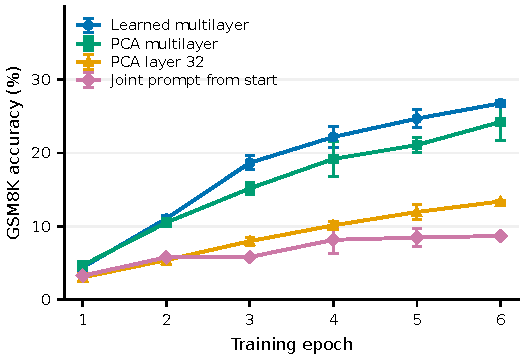
\includegraphics[width=.66\linewidth]{figures/representation_identity_sd.pdf}
\caption{\textbf{Identity-clock robustness.} The four models from Figure~\ref{fig:representationcomparison}, evaluated with $t=\tau$ and 32 steps. Points average seeds 42/123 (bars: seed SD). Each epoch uses one trained checkpoint per arm. Numerical values appear in Table~\ref{tab:representationcurvevalues}.}
\label{fig:representationidentity}
\end{figure}

All four arms start from the same seed-42 backbone initialization, use 2,434,330 training rows, and preserve effective batch 512. All answer representations are whitened and 1,024-dimensional. The first three arms use frozen Qwen prompt activations; the fourth uses learned multilayer answer latents and a randomly initialized prompt encoder trained jointly from epoch zero. All select backbone EMA $0.999$, and the fourth selects prompt EMA $0.999$. The PCA multilayer run changes from two to four GPUs during training while maintaining that batch size. Each arm has one training run; seed variation in the figures measures sampling randomness only. The comparisons isolate projector choice at fixed layers and layer choice under PCA, without estimating their interaction. Paired intervals in the main text use 4,000 problem-bootstrap replicates and the four matched epoch-six generation seeds.

\paragraph{Representation-ablation curves.}
Table~\ref{tab:representationcurvevalues} gives all points and error bars in Figures~\ref{fig:representationcomparison} and~\ref{fig:representationidentity}, followed by the four-seed epoch-six summary discussed in Sections~\ref{sec:representationablations} and~\ref{sec:conditionalencoding}. The curves use seeds 42/123; the endpoint summary adds 456/789. Error bars and parenthesized values are sample SDs across their respective generation seeds. Both use 32 steps and backbone EMA $0.999$; The controls above apply to both clocks.

\begin{table}[htbp]
\centering\small
\setlength{\tabcolsep}{5pt}
\caption{Numerical learning curves and endpoint summary for Figures~\ref{fig:representationcomparison} and~\ref{fig:representationidentity}: mean GSM8K accuracy (\%) with sample seed SD in parentheses. Curves use two seeds (42/123); the final block reports the four-seed epoch-six comparison (42/123/456/789). The final column trains the prompt encoder jointly from epoch zero; the other three retain Qwen prompt conditioning.}
\label{tab:representationcurvevalues}
\begin{tabular}{@{}rrrrr@{}}
\toprule
Epoch & \shortstack{Learned\\16/24/32} & \shortstack{PCA\\16/24/32} & \shortstack{PCA\\layer 32} & \shortstack{Epoch-0 joint\\prompt training} \\
\midrule
\multicolumn{5}{@{}l}{$t=\tau^2$}\\
1 & 3.75 {\scriptsize (0.05)} & 4.85 {\scriptsize (0.75)} & 2.65 {\scriptsize (0.11)} & 2.46 {\scriptsize (0.05)} \\
2 & 12.40 {\scriptsize (0.27)} & 11.18 {\scriptsize (0.16)} & 5.50 {\scriptsize (0.70)} & 3.98 {\scriptsize (1.02)} \\
3 & 20.17 {\scriptsize (0.54)} & 16.38 {\scriptsize (0.32)} & 8.64 {\scriptsize (0.43)} & 3.68 {\scriptsize (0.16)} \\
4 & 26.61 {\scriptsize (0.86)} & 21.49 {\scriptsize (0.80)} & 7.47 {\scriptsize (0.05)} & 7.77 {\scriptsize (1.02)} \\
5 & 29.95 {\scriptsize (0.21)} & 25.85 {\scriptsize (0.21)} & 9.82 {\scriptsize (0.16)} & 7.54 {\scriptsize (1.45)} \\
6 & 31.01 {\scriptsize (0.43)} & 28.39 {\scriptsize (0.27)} & 11.68 {\scriptsize (0.21)} & 8.61 {\scriptsize (0.05)} \\
\addlinespace
\multicolumn{5}{@{}l}{$t=\tau$}\\
1 & 4.40 {\scriptsize (0.75)} & 4.66 {\scriptsize (0.48)} & 3.03 {\scriptsize (0.54)} & 3.26 {\scriptsize (0.11)} \\
2 & 11.03 {\scriptsize (0.38)} & 10.50 {\scriptsize (0.16)} & 5.38 {\scriptsize (0.54)} & 5.76 {\scriptsize (0.00)} \\
3 & 18.65 {\scriptsize (0.96)} & 15.16 {\scriptsize (0.86)} & 7.96 {\scriptsize (0.54)} & 5.80 {\scriptsize (0.05)} \\
4 & 22.18 {\scriptsize (1.45)} & 19.18 {\scriptsize (2.36)} & 10.12 {\scriptsize (0.48)} & 8.15 {\scriptsize (1.88)} \\
5 & 24.68 {\scriptsize (1.23)} & 21.08 {\scriptsize (0.96)} & 11.94 {\scriptsize (1.02)} & 8.45 {\scriptsize (1.23)} \\
6 & 26.76 {\scriptsize (0.43)} & 24.22 {\scriptsize (2.52)} & 13.38 {\scriptsize (0.16)} & 8.68 {\scriptsize (0.16)} \\
\addlinespace
\multicolumn{5}{@{}l}{Epoch-six summary: $t=\tau^2$, four seeds}\\
6 & 30.76 {\scriptsize (0.39)} & 28.43 {\scriptsize (0.19)} & 11.20 {\scriptsize (0.56)} & 8.70 {\scriptsize (0.33)} \\
\addlinespace
\bottomrule
\end{tabular}
\end{table}

\section{Inference clocks and reconstruction diagnostics}
\label{app:inferenceclocks}

\subsection{Local clocks, time embeddings, and samplers}

\paragraph{Local corruption and time embeddings.}
The local clocks in Section~\ref{sec:clocks} assign each group its own Gaussian corruption, $z_{\bm t}^{(\ell)}=t_\ell z_{\mathrm{clean}}^{(\ell)}+(1-t_\ell)\sigma\epsilon^{(\ell)}$. The three time embedders are identical copies of the selected scalar-time checkpoint weights:
\begin{equation}
 \bar e_\theta^{\mathrm{time}}(\bm t)
 =\frac{1}{3}\sum_{\ell\in\{16,24,32\}}e_{\theta,\ell}^{\mathrm{time}}(t_\ell),
 \qquad e_{\theta,\ell}^{\mathrm{time}}=e_\theta^{\mathrm{time}}.
 \label{eq:asynctimeembedding}
\end{equation}
All other tensors are unchanged. The embedding outputs are weighted equally, irrespective of the 256/256/512 group widths, with the mean accumulated in FP64 before casting back to model dtype. The resulting embedding is a shared network condition, not a separate Transformer for each group. In particular, permuting the three exponents preserves this conditioning average while changing the coordinate groups to which the local velocity factors apply. Because the group widths differ, that permutation need not preserve total latent noise energy.

\paragraph{Sampling grid and conditioning.}
For $S$ denoising steps, we set $\tau_0=0$, $\tau_S=1$, and use the same logit-normal-quantile grid across schedules:
\begin{equation}
 \tau_r=\operatorname{sigmoid}\!\left[-1.5+0.8\Phi^{-1}(r/S)\right],
 \qquad 0<r<S.
\end{equation}
The base $\tau$ grid is fixed across schedule and sampler comparisons. For the ODE baseline, we retain the full derivative $f'_\ell(\tau)=\gamma_\ell\tau^{\gamma_\ell-1}$ in Eq.~\eqref{eq:asyncsampler}, with the endpoint denominator $\Delta_{t_{\ell,r}}=\max(1-\tau_r^{\gamma_\ell},0.05)$. Question states remain clean, and recurrent self-conditioning carries the previous endpoint prediction to the next call. Changing the clock therefore alters both the integration grid in local time and the prediction history. One shared denoiser call updates all groups; the terminal token-decoding call remains separate.

\paragraph{Stochastic-sampler implementation.}
\label{app:samplerimplementation}
The labels \emph{Stochastic (DMD2)} and \emph{Stochastic (EDM)} identify the update families in Eqs.~\eqref{eq:asyncdmd2}--\eqref{eq:asyncchurnforward}. Both use the same destination grid as ODE, $\sigma=2$, and default local-clock exponents $(2.5,2,1.5)$; the schedule comparison varies these powers. They operate on the fixed supervised and NFT endpoints without retraining or checkpoint reselection.

For DMD2-style sampling, the fresh-noise multiplier is one ($\eta=1$): the injected standard deviation in group $\ell$ is exactly $\sigma(1-t_{\ell,r+1})$. Each nonterminal step draws fresh Gaussian noise after predicting the clean endpoint, including the first step. At $r=S-1$, Eq.~\eqref{eq:asyncdmd2} gives $z_S=\widehat z_{\mathrm{clean},S-1}$, and no noise is drawn.

For EDM-style sampling, let $G(u)=\operatorname{sigmoid}[-1.5+0.8\Phi^{-1}(u)]$ for $0<u<1$, with $G(0)=0$ and $G(1)=1$. On interior transitions $1\leq r\leq S-2$, contract the \emph{uniform quantile index} by a factor of $0.7$:
\begin{equation}
 \bar\tau_r=G(0.7r/S),\qquad
 \bar t_{\ell,r}=f_\ell(\bar\tau_r),\qquad
 \tau_r=G(r/S).
 \label{eq:indexchurnclock}
\end{equation}
Thus $\bar\tau_r$ is generally not $0.7\tau_r$. The variance in Eq.~\eqref{eq:asyncchurnback} follows by matching the forward Gaussian corruption: scaling $z_r^{(\ell)}$ by $\alpha_{\ell,r}$ gives signal coefficient $\bar t_{\ell,r}$, and independent noise supplies the remaining variance. This is nonnegative for $0\leq\bar t_{\ell,r}\leq t_{\ell,r}<1$. The denoiser is evaluated at these noisier times, using the same averaged time embeddings as above. Eq.~\eqref{eq:asyncchurnforward} uses the finite increment $t_{\ell,r+1}-\bar t_{\ell,r}$ and denominator $1-\bar t_{\ell,r}$, without the derivative factor or denominator clamp of Eq.~\eqref{eq:asyncsampler}.

At the initial transition, churn is bypassed: $\bar z_0=z_0$ and $\bar t_{\ell,0}=0$, followed by Eq.~\eqref{eq:asyncchurnforward}. At the terminal transition, churn is again bypassed; the denoiser is evaluated at the current state and times, and its clean prediction is used directly as $z_S$. We restore prompt positions after noise injection and every state update, and retain the previous guided clean prediction for self-conditioning. The noise-injection and local Euler rules adapt EDM's churn principle; the quantile-index contraction and first-order update differ from its original sampler.

Both stochastic samplers initialize from the same seeded Gaussian distribution as ODE, use $S$ denoiser calls and one separate terminal decoder call, and add no terminal noise. Fresh noise comes from a separate per-batch CUDA generator, seeded by $(s+1{,}000{,}003+b\cdot1{,}000{,}003)\bmod(2^{63}-1)$, where $s$ is the evaluation seed and $b$ the first benchmark-row index in the batch. DMD2-style sampling applies $S-1$ fresh draws. EDM-style sampling consumes the first draw without applying it and applies the $S-2$ interior draws. The network runs in BF16, latent updates in FP32, and the time-embedding mean in FP64 before casting back.

The stochastic samplers decode their final predicted-clean state, while the ODE baseline decodes its final Euler-updated state. Comparisons with ODE therefore include this terminal-rule difference, as well as the distinct update formulas, and do not isolate the effect of fresh noise alone.

\subsection{Schedule comparisons}
\label{app:schedulecomparisons}
All test-set schedule comparisons use CEDR-L epoch 21, 32 denoising steps, CFG 1, SCCFG 2 for GSM8K and 3 for MATH500, backbone/prompt EMA $0.9999/0.9999$, batch size 32, and seeds 42/123. GSM8K CEDR-L uses the same learned projectors as CEDR-B. Scores use numerical-answer accuracy for all 1,319 GSM8K test problems and Math-Verify for all 500 MATH500 problems (Appendix~\ref{app:experimentdetails}); PRM800K remains a secondary scorer. Table~\ref{tab:inferenceclocks} summarizes all three samplers; Table~\ref{tab:stochasticclockdetail} gives the individual stochastic-sampler seed results and pass@2. Bold marks the highest mean among the four schedules within each dataset/sampler. The stochastic comparison uses the same checkpoints and seeds as the ODE references and covers test sets at epoch 21; it does not add validation-set or NFT schedule evaluations. Thus both datasets use the same guidance as their headline results.

Table~\ref{tab:inferenceclockfull} retains the original ODE validation sweep at SCCFG 2 for both datasets, alongside the test results at headline guidance. The 500-problem MATH validation set comes from the same original MATH test pool as MATH500, excluding its questions, whereas our GSM8K validation set comprises held-out original training questions. We therefore regard the MATH validation comparison as more directly matched to its benchmark's source distribution. Both validation sets give their highest observed mean to $(2.5,2,1.5)$. On GSM8K validation, its advantages over $(2,2,2)$ and $(1.5,2,2.5)$ are 0.75 and 0.50 percentage points, respectively, with paired 95\% intervals $[-0.30,1.85]$ and $[-0.60,1.55]$. The small differences among these nonidentity clocks do not establish a unique best schedule.

\begin{table}[htbp]
\centering\small
\caption{Four-schedule CEDR-L epoch-21 comparison: mean pass@1 (\%) with sample seed SD in parentheses, over seeds 42/123 with ODE sampling at 32 denoising steps. Validation uses SCCFG 2; test uses SCCFG 2 for GSM8K and 3 for MATH500. Validation sets contain 1,000 GSM8K and 500 MATH problems. Test columns reproduce the ODE entries and SDs from Table~\ref{tab:inferenceclocks}. Bold marks each column maximum, including ties.}
\label{tab:inferenceclockfull}
\begin{tabular}{lrrrr}
\toprule
& \multicolumn{2}{c}{Validation} & \multicolumn{2}{c}{Test} \\
\cmidrule(lr){2-3}\cmidrule(lr){4-5}
Clock powers & GSM8K & MATH & GSM8K & MATH500 \\
\midrule
$(1,1,1)$ & 64.60 {\scriptsize (0.57)} & 15.40 {\scriptsize (0.28)} & 52.62 {\scriptsize (0.75)} & 16.70 {\scriptsize (0.42)} \\
$(2,2,2)$ & 72.85 {\scriptsize (0.21)} & 17.80 {\scriptsize (0.57)} & 59.97 {\scriptsize (0.64)} & 18.80 {\scriptsize (0.85)} \\
$(1.5,2,2.5)$ & 73.10 {\scriptsize (0.85)} & 18.30 {\scriptsize (0.14)} & \textbf{60.08} {\scriptsize (0.38)} & 18.50 {\scriptsize (0.14)} \\
$(2.5,2,1.5)$ & \textbf{73.60} {\scriptsize (0.28)} & \textbf{18.70} {\scriptsize (0.14)} & 59.78 {\scriptsize (0.16)} & \textbf{19.70} {\scriptsize (0.42)} \\
\bottomrule
\end{tabular}
\end{table}

\paragraph{Stochastic schedule comparisons.}
Table~\ref{tab:stochasticclockdetail} gives individual seed results and pass@2 for both stochastic samplers. Pass@1 averages the two draws within each problem and then averages problems equally; pass@2 is the fraction of problems solved by either draw. Sample SD describes variation between the two full-benchmark seed accuracies, rather than problem-bootstrap uncertainty.

\begin{table}[htbp]
\centering\small
\setlength{\tabcolsep}{4pt}
\caption{Detailed stochastic-sampler schedule results underlying Table~\ref{tab:inferenceclocks}: individual seed accuracies, mean pass@1 with sample seed SD, and oracle pass@2, all in percent. Settings match the 32-step ODE comparison, with SCCFG 2 for GSM8K and 3 for MATH500; each problem has two generated solutions.}
\label{tab:stochasticclockdetail}
\begin{tabular}{@{}llrrrr@{}}
\toprule
Sampler & Clock powers & Seed 42 & Seed 123 & Mean pass@1 & pass@2 \\
\midrule
\multicolumn{6}{l}{\textbf{GSM8K}} \\
\multirow{4}{*}{Stochastic (EDM)} & $(1,1,1)$ & 59.82 & 59.74 & 59.78 {\scriptsize($\pm 0.05$)} & 69.60 \\
 & $(2,2,2)$ & 61.18 & 62.47 & 61.83 {\scriptsize($\pm 0.91$)} & 69.83 \\
 & $(1.5,2,2.5)$ & 63.00 & 63.84 & 63.42 {\scriptsize($\pm 0.59$)} & 70.81 \\
 & $(2.5,2,1.5)$ & 64.67 & 64.22 & \textbf{64.44} {\scriptsize($\pm 0.32$)} & 71.87 \\
\addlinespace[3pt]
\multirow{4}{*}{Stochastic (DMD2)} & $(1,1,1)$ & 60.80 & 60.20 & 60.50 {\scriptsize($\pm 0.43$)} & 69.75 \\
 & $(2,2,2)$ & 64.75 & 64.97 & 64.86 {\scriptsize($\pm 0.16$)} & 71.04 \\
 & $(1.5,2,2.5)$ & 67.10 & 65.88 & 66.49 {\scriptsize($\pm 0.86$)} & 72.10 \\
 & $(2.5,2,1.5)$ & 66.72 & 66.64 & \textbf{66.68} {\scriptsize($\pm 0.05$)} & 72.40 \\
\midrule
\multicolumn{6}{l}{\textbf{MATH500 (Math-Verify)}} \\
\multirow{4}{*}{Stochastic (EDM)} & $(1,1,1)$ & 18.40 & 20.80 & 19.60 {\scriptsize($\pm 1.70$)} & 27.20 \\
 & $(2,2,2)$ & 18.40 & 15.20 & 16.80 {\scriptsize($\pm 2.26$)} & 25.00 \\
 & $(1.5,2,2.5)$ & 20.60 & 19.20 & 19.90 {\scriptsize($\pm 0.99$)} & 28.40 \\
 & $(2.5,2,1.5)$ & 20.40 & 22.80 & \textbf{21.60} {\scriptsize($\pm 1.70$)} & 30.20 \\
\addlinespace[3pt]
\multirow{4}{*}{Stochastic (DMD2)} & $(1,1,1)$ & 19.20 & 23.00 & 21.10 {\scriptsize($\pm 2.69$)} & 29.40 \\
 & $(2,2,2)$ & 22.20 & 25.60 & 23.90 {\scriptsize($\pm 2.40$)} & 31.80 \\
 & $(1.5,2,2.5)$ & 23.20 & 26.80 & 25.00 {\scriptsize($\pm 2.55$)} & 33.20 \\
 & $(2.5,2,1.5)$ & 26.40 & 29.40 & \textbf{27.90} {\scriptsize($\pm 2.12$)} & 36.20 \\
\bottomrule
\end{tabular}
\end{table}

\paragraph{Paired schedule differences.}
Table~\ref{tab:clockpaireddifferences} compares $(2.5,2,1.5)$ against $(2,2,2)$ and $(1.5,2,2.5)$ within each sampler. Its GSM8K advantage over $(2,2,2)$ has a positive paired interval for both stochastic samplers, while the corresponding ODE interval includes zero. On MATH500, DMD2-style sampling gives positive paired intervals against both comparators: $+4.00$ points over $(2,2,2)$ and $+2.90$ over $(1.5,2,2.5)$. The EDM-style gain over $(2,2,2)$ also has a positive interval, while its reverse-versus-forward interval and both ODE intervals include zero. Neither stochastic sampler separates the two asynchronous clocks on GSM8K with these two seeds. The shared-square clock is also not uniformly preferable: under EDM-style sampling, MATH500 accuracy falls from 19.60\% with identity clocks to 16.80\% with shared-square clocks.

\begin{table}[htbp]
\centering\small
\setlength{\tabcolsep}{5pt}
\caption{Paired pass@1 differences, in percentage points, for $(2.5,2,1.5)$ minus the listed comparator clock within each sampler. Brackets give 95\% problem-bootstrap intervals. All comparisons use CEDR-L epoch 21, 32 steps, SCCFG 2 for GSM8K / 3 for MATH500, and seeds 42/123.}
\label{tab:clockpaireddifferences}
\begin{tabular}{@{}llrr@{}}
\toprule
Sampler & Comparator & GSM8K & MATH500 \\
\midrule
\multirow{2}{*}{ODE} & $(2,2,2)$ & $-0.19\;[-1.06,+0.68]$ & $+0.90\;[-1.00,+2.90]$ \\
 & $(1.5,2,2.5)$ & $-0.30\;[-1.18,+0.57]$ & $+1.20\;[-0.90,+3.40]$ \\
\addlinespace[3pt]
\multirow{2}{*}{Stochastic (EDM)} & $(2,2,2)$ & $+2.62\;[+1.25,+4.02]$ & $+4.80\;[+2.50,+7.10]$ \\
 & $(1.5,2,2.5)$ & $+1.02\;[-0.23,+2.27]$ & $+1.70\;[-0.60,+4.10]$ \\
\addlinespace[3pt]
\multirow{2}{*}{Stochastic (DMD2)} & $(2,2,2)$ & $+1.82\;[+0.53,+3.07]$ & $+4.00\;[+1.40,+6.50]$ \\
 & $(1.5,2,2.5)$ & $+0.19\;[-1.02,+1.40]$ & $+2.90\;[+0.40,+5.30]$ \\
\bottomrule
\end{tabular}
\end{table}

Intervals use 4,000 paired problem-bootstrap replicates with bootstrap seed 20260918, resampling the same problem indices across compared settings and retaining both draws per problem. They quantify uncertainty across problems for the fixed checkpoints and draws, do not estimate training variance, and do not account for testing multiple schedules. Within each sampler, only the clocks change. Across samplers, comparisons include the distinct integration and terminal-decoding rules described in Appendix~\ref{app:samplerimplementation}.

\subsection{Layer decomposition and reconstruction sensitivity}
We probe a trained CEDR-B model by corrupting one group of clean gold-solution latents, predicting the clean representation, and decoding it to tokens. A matched control replaces the layer groups by eight random partitions of the same 256/256/512 widths, keeping the assigned times and injected Gaussian energy fixed. Figure~\ref{fig:layerreconstruction} shows that the actual groups have different reconstruction sensitivities: perturbing layer-16 features is more damaging than perturbing deeper features, with the clearest contrast against layer 24. Random grouping attenuates these contrasts. The layer decomposition thus exposes structure that is obscured when coordinates are grouped arbitrarily.

\begin{figure}[htbp]
\centering
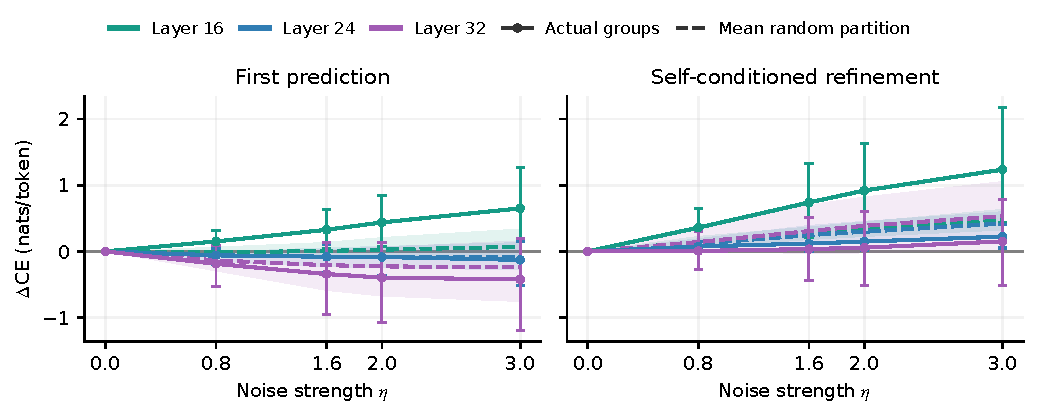
\includegraphics[width=\linewidth]{figures/layer_reconstruction_random.pdf}
\caption{\textbf{Layer groups expose distinct reconstruction sensitivities.} CEDR-B epoch 18 on 64 GSM8K validation problems. Solid curves perturb actual layer groups; dashed curves average eight random partitions with matched widths, times, and injected Gaussian energy. Colors identify the corresponding layer or control slot. Decoder CE changes are relative to the same pass's clean-input prediction: first without answer self-conditioning (left), then after one refinement on the same corrupted input (right). Bars show 95\% CIs; shading is the range of random-partition means, not a confidence interval. Table~\ref{tab:reconstructioncurvevalues} gives every plotted value.}
\label{fig:layerreconstruction}
\end{figure}

\paragraph{Reconstruction intervention.}
Figure~\ref{fig:layerreconstruction} uses CEDR-B epoch 18, backbone/prompt EMA $0.9999/0.9999$, SCCFG 1, noise seeds 42/123, and a fixed 64-problem GSM8K validation panel. For a selected group $\ell$, we set $t_\ell=2/[2+\eta\,\mathrm{RMS}(z_{\mathrm{clean}}^{(\ell)})]$ and replace its assistant-content coordinates by $t_\ell z_{\mathrm{clean}}^{(\ell)}+2(1-t_\ell)\epsilon^{(\ell)}$, for $\eta\in\{0.8,1.6,2,3\}$. Other coordinates, question positions, terminal tokens, and padding remain clean. The model predicts the full clean latent, which its own token head decodes. The second pass reuses the same corrupted input with the first prediction as self-conditioning; it is not another integration step. CE averages gold-token losses within each problem, then noise seeds and problems equally. Negative changes mean lower CE than the clean-input \emph{prediction} baseline, not a negative loss.

The random control uses eight fixed NumPy PCG64 partitions (seeds 20260918--20260925). Each control slot retains its true-group time and injected Gaussian energy; random-subset RMS is recorded but does not recalibrate the intervention. At $\eta=3$, after self-conditioning, the true-group layer-16 minus layer-24 CE contrast exceeds the corresponding mean-random contrast by 0.967 nats/token (paired 95\% CI $[0.168,1.890]$). The layer-16 minus layer-32 excess is 1.149 ($[0.061,2.241]$), with weaker evidence at lower noise and in the first prediction. Random partitions are averaged within problem before resampling; they are not additional independent problems.

\paragraph{Interpretation.}
For $0<\tau<1$, our chosen powers give $t_{16}<t_{24}<t_{32}$: layer 16 becomes clean relatively later, while all groups reach their endpoint together. One possible explanation is that the more sensitive layer-16 representation benefits from being reconstructed with cleaner deeper-layer features available as context. This is a hypothesis about coordination between representations, rather than a consequence of the local probe. The probe motivates investigating layer-dependent denoising, but further experiments are needed to establish whether this proposed mechanism explains its sampling benefits.

\paragraph{Reconstruction-sensitivity curves.}
Table~\ref{tab:reconstructioncurvevalues} reproduces the means, error bars, and shaded ranges in Figure~\ref{fig:layerreconstruction}. The zero-noise points are identically zero because each condition is compared with its own pass's clean-input baseline. Random-partition ranges describe the eight partition means, not uncertainty intervals.

\begin{table}[htbp]
\centering\small
\setlength{\tabcolsep}{5pt}
\caption{Numerical values for Figure~\ref{fig:layerreconstruction}, in nats/token. Actual-group entries give $\Delta$CE and its 95\% problem-bootstrap CI; random-group entries give the mean over eight matched partitions and the minimum/maximum partition means. Noise strength is $\eta$; the layer identifies the matched group width.}
\label{tab:reconstructioncurvevalues}
\begin{tabular}{@{}rrcc@{}}
\toprule
Layer & $\eta$ & Actual group [95\% CI] & Random mean [min, max] \\
\midrule
\multicolumn{4}{@{}l}{\textit{First prediction}}\\
16 & 0 & $0.000\ [0.000, 0.000]$ & $0.000\ [0.000, 0.000]$ \\
16 & 0.8 & $0.151\ [-0.006, 0.315]$ & $-0.015\ [-0.053, 0.064]$ \\
16 & 1.6 & $0.327\ [0.045, 0.633]$ & $0.008\ [-0.057, 0.136]$ \\
16 & 2 & $0.439\ [0.080, 0.848]$ & $0.026\ [-0.075, 0.209]$ \\
16 & 3 & $0.651\ [0.158, 1.272]$ & $0.071\ [-0.087, 0.340]$ \\
24 & 0 & $0.000\ [0.000, 0.000]$ & $0.000\ [0.000, 0.000]$ \\
24 & 0.8 & $-0.059\ [-0.201, 0.050]$ & $-0.065\ [-0.154, -0.010]$ \\
24 & 1.6 & $-0.081\ [-0.314, 0.103]$ & $-0.080\ [-0.231, 0.055]$ \\
24 & 2 & $-0.085\ [-0.365, 0.131]$ & $-0.084\ [-0.245, 0.075]$ \\
24 & 3 & $-0.128\ [-0.512, 0.154]$ & $-0.078\ [-0.279, 0.134]$ \\
32 & 0 & $0.000\ [0.000, 0.000]$ & $0.000\ [0.000, 0.000]$ \\
32 & 0.8 & $-0.188\ [-0.533, 0.087]$ & $-0.136\ [-0.294, -0.050]$ \\
32 & 1.6 & $-0.342\ [-0.950, 0.140]$ & $-0.208\ [-0.588, 0.028]$ \\
32 & 2 & $-0.395\ [-1.075, 0.140]$ & $-0.226\ [-0.675, 0.065]$ \\
32 & 3 & $-0.424\ [-1.189, 0.194]$ & $-0.241\ [-0.757, 0.160]$ \\
\addlinespace
\multicolumn{4}{@{}l}{\textit{Self-conditioned refinement}}\\
16 & 0 & $0.000\ [0.000, 0.000]$ & $0.000\ [0.000, 0.000]$ \\
16 & 0.8 & $0.360\ [0.073, 0.653]$ & $0.142\ [0.060, 0.226]$ \\
16 & 1.6 & $0.740\ [0.211, 1.330]$ & $0.271\ [0.180, 0.369]$ \\
16 & 2 & $0.920\ [0.289, 1.637]$ & $0.334\ [0.226, 0.446]$ \\
16 & 3 & $1.237\ [0.436, 2.179]$ & $0.469\ [0.324, 0.636]$ \\
24 & 0 & $0.000\ [0.000, 0.000]$ & $0.000\ [0.000, 0.000]$ \\
24 & 0.8 & $0.075\ [0.006, 0.150]$ & $0.117\ [0.052, 0.192]$ \\
24 & 1.6 & $0.119\ [0.005, 0.237]$ & $0.247\ [0.115, 0.392]$ \\
24 & 2 & $0.149\ [0.019, 0.285]$ & $0.298\ [0.132, 0.455]$ \\
24 & 3 & $0.223\ [0.051, 0.406]$ & $0.422\ [0.211, 0.600]$ \\
32 & 0 & $0.000\ [0.000, 0.000]$ & $0.000\ [0.000, 0.000]$ \\
32 & 0.8 & $0.007\ [-0.267, 0.295]$ & $0.142\ [0.001, 0.348]$ \\
32 & 1.6 & $0.036\ [-0.440, 0.508]$ & $0.307\ [-0.031, 0.701]$ \\
32 & 2 & $0.056\ [-0.509, 0.602]$ & $0.388\ [-0.023, 0.822]$ \\
32 & 3 & $0.152\ [-0.515, 0.792]$ & $0.533\ [0.030, 1.057]$ \\
\addlinespace
\bottomrule
\end{tabular}
\end{table}

\section{NFT implementation and gold-anchor analysis}
\label{app:nftdetails}

\subsection{Collection, rewards, and forward corruption}

Each collection round draws 24 prompt groups from the applicable training population; coding uses the screened reward cohort in Appendix~\ref{app:nfttraining}. The old policy produces 15 candidates per group using 32 Euler denoising steps, synchronous identity clocks, the logit-normal-quantile grid of Appendix~\ref{app:inferenceclocks}, initial noise scale two, prompt CFG one, and SCCFG two. Self-conditioning is recurrent during collection. Terminal token decoding is greedy and uses the same SCCFG scale. We save the terminal latent endpoint and its decoded answer length; generated text is used for reward evaluation without re-encoding it through Qwen. Each group additionally receives one gold endpoint from the fixed answer cache. No Qwen Transformer forward is required during NFT.

The generated reward is $0.75$ for a correct final answer and zero otherwise, while the gold reward is one. GSM8K uses numerical-answer correctness. MATH uses Math-Verify 0.9.0 with a five-second timeout; unparsed predictions, exceptions, and timeouts receive zero. Coding correctness requires all retained native training assertions to pass (Appendix~\ref{app:nfttraining}). All-correct generated groups are excluded before computing normalization statistics. For retained group $b$ and candidate $m$, define
\begin{equation}
 A_{bm}=\operatorname{clip}\!\left(
 \frac{R_{bm}-\bar R_b}{\sigma_R+10^{-4}},-5,5\right),
 \qquad
 \rho_{bm}=\operatorname{clip}\!\left(\frac12+\frac{A_{bm}}{10},0,1\right),
 \label{eq:nftrewardnormalization}
\end{equation}
where $\bar R_b$ averages all 16 endpoints and $\sigma_R$ is the population standard deviation of the retained \emph{raw} rewards across the complete collection round. Discarded groups do not enter these statistics. All-incorrect groups remain informative because they include a gold endpoint. The GSM8K implementations additionally stop before an update if an entire round has zero correct generations; the MATH and coding implementations disable that round-level guard and permit gold-anchored updates. A round with no retained groups supplies no optimizer update.

Correct generations remain in mixed groups. Because gold has a higher raw reward than correct generations, even all-correct groups would supply a gold-versus-generation preference if retained. Filtering removes those groups to concentrate updates on observed failures. The higher gold reward favors the reference reasoning trace within the latent objective, whereas generated-solution rewards depend only on final-answer correctness.

For each retained endpoint, draw eight independent time/noise/self-conditioning records, yielding at most $24\times16\times8=3072$ records per update. Each record draws $t=\operatorname{sigmoid}(-1.5+0.8\xi)$, with $\xi\sim\mathcal N(0,1)$, independently of the rollout grid. All representation groups use this same time, with unit group weights. Corrupt answer latents using Eq.~\eqref{eq:methodinterpolant} and convert predictions and endpoint targets using $\Delta_t=\max(1-t,0.05)$. Each policy restores its own clean prompt states, while endpoint, noise, answer states, and masks are shared across roles. Masks include the first EOS token and exclude prompt and subsequent padding positions.

\subsection{SCCFG construction and exact loss}

For each record, sample $b_{\mathrm{sc}}\sim\mathrm{Bernoulli}(0.5)$ and $\log(1+g)\sim\mathrm{Uniform}(\log1.5,\log6)$. Use the same $b_{\mathrm{sc}},g$ for current, old, and reference roles. Each role first predicts a clean endpoint under zero answer self-conditioning, restores its own clean prompt, and detaches that prediction. The main forward receives $b_{\mathrm{sc}}$ times the bootstrap prediction in answer positions; prompt positions remain clean regardless of $b_{\mathrm{sc}}$. The guidance-scale input $g$ is supplied to both passes. Convert both predictions to velocities and apply Eq.~\eqref{eq:nftcorrectedfield}.

Only the current main forward carries gradients. Bootstrap predictions, the entire guidance correction, old/reference computations, sampled endpoints, and data targets are detached, giving $\nabla_\Theta\widetilde v_{\mathrm{cur}}=\nabla_\Theta v_{\mathrm{cur}}^{\mathrm{main}}$ under the implemented differentiation. The current prompt encoder receives the main-forward chain-rule gradient, including its use as the clean condition. Its output gradients are accumulated across records and propagated through the shared prompt graph. This implements the same detached construction as the ELF guidance-adjusted target: $\widetilde v_{\mathrm{cur}}-u_t^{\mathrm{stab}}$ equals $v_{\mathrm{cur}}^{\mathrm{main}}-\sg[u_t^{\mathrm{stab}}+b_{\mathrm{sc}}(1-g^{-1})(v_{\mathrm{cur}}^{\mathrm{main}}-v_{\mathrm{cur}}^0)]$ when $u_t^{\mathrm{stab}}$ is detached. Removing the stop-gradient from the correction would change the update.

Let $b$ index retained training records and $i$ full-canvas token positions. With $d=1024$, define $N_{\mathrm{tok}}=\sum_{bi}M_{bi}$ across all ranks and microbatches of the update. Define
\begin{equation}
 \mathcal S(e;\omega)=\sum_{bi}M_{bi}\omega_b\frac{\|e_{bi}\|_2^2}{d}.
 \label{eq:nfttokensum}
\end{equation}
With $e_c=\widetilde v_{\mathrm{cur}}-\sg(u_t^{\mathrm{stab}})$ and $e_o=\sg(\widetilde v_{\mathrm{old}})-\sg(u_t^{\mathrm{stab}})$, the beta-one residuals are $e_+=e_c$ and $e_-=2e_o-e_c$. The executed loss is
\begin{equation}
 \mathcal L_{\mathrm{NFT}}=
 \frac{5}{N_{\mathrm{tok}}}\bigl[\mathcal S(e_+;\rho)+\mathcal S(e_-;1-\rho)\bigr]
 +\frac{0.1}{N_{\mathrm{tok}}}\mathcal S\bigl(\widetilde v_{\mathrm{cur}}-\sg(\widetilde v_{\mathrm{ref}});1\bigr).
 \label{eq:nftexecutedloss}
\end{equation}
This averages coordinates and valid tokens, rather than averaging a separate mean for each solution. Gradients are summed across ranks using the same update-wide denominator. The reference term is a squared-velocity penalty. We omit the adaptive residual normalization of the original DiffusionNFT implementation \citep{diffusionnft}; no decoder CE, prompt MSE, or separate correct-solution flow auxiliary loss is added.

\subsection{Policy roles and old-policy updates}
\label{sec:nftjoint}

Appendix~\ref{app:nfttraining} specifies initialization, trainable components, and optimizer settings.

The parameterization in Section~\ref{sec:conditionalencoding} makes the question tokens the external condition for all roles. Thus the current, old, and reference policies use their respective encoders $P_\phi$, $P_{\phi_{\mathrm{old}}}$, and $P_{\phi_{\mathrm{ref}}}$ while being compared under the same question $q$.

After successful update $n$, both old-policy components are updated by
\begin{equation}
 \Theta_{\mathrm{old}}\leftarrow \alpha_n\Theta_{\mathrm{old}}+(1-\alpha_n)\Theta_{\mathrm{cur}},
 \qquad \alpha_n=\begin{cases}\min(0.001n,0.5),&n<400,\\0.4,&n\ge400.\end{cases}
 \label{eq:nftoldema}
\end{equation}
The reference remains at initialization. The evaluation EMAs specified in Appendix~\ref{app:nfttraining} are distinct from this old-policy retention schedule.

\subsection{Proof and interpretation of gold anchoring}
\label{app:nftgoldproof}

\begin{proof}[Proof of Lemma~\ref{lem:goldanchor}]
All expectations below condition on $\mathcal H$ and a gold endpoint, so $f,h,\rho_G$ are fixed. Let $\sigma_G^2=\E[\|U-m_G\|_2^2\mid\mathcal H,\mathrm{gold}]$. Conditional variance decomposition gives
\begin{equation}
 \E[\ell_1(f,h;U,\rho_G)\mid\mathcal H,\mathrm{gold}]
 =\rho_G\|f-m_G\|_2^2
 +(1-\rho_G)\|f-(2h-m_G)\|_2^2+\sigma_G^2.
\end{equation}
For any vectors $a,b$, the identity $\omega\|f-a\|^2+(1-\omega)\|f-b\|^2=\|f-[\omega a+(1-\omega)b]\|^2+\omega(1-\omega)\|a-b\|^2$ completes the square. Substituting $a=m_G$, $b=2h-m_G$, and $\omega=\rho_G$ yields Eq.~\eqref{eq:nftgoldanchor}, with
\begin{equation}
 C_{\mathcal H}=\sigma_G^2+4\rho_G(1-\rho_G)\|m_G-h\|_2^2.
\end{equation}
The anchor weights $2\rho_G-1$ and $2(1-\rho_G)$ are nonnegative and sum to one.
\end{proof}

\paragraph{Random coefficients and reference interpretation.}
In the executed reward mapping, the gold raw reward exceeds its group's mean, so $\rho_G\in(1/2,1]$. Its value depends on the group's generations and the retained population. The conditioning information $\mathcal H$ therefore includes the realized coefficient and any retention information used to define the population; $m_G$ is computed under that same conditional distribution. The lemma does not assume coefficient--target independence. If that independence holds given state, time, and question, the coefficient can be removed from the conditioning of $m_G$. Identifying $m_G$ with a reference field requires the stronger idealization that the reference matches this gold posterior target under the same conditioning and corruption law. Correct final answers alone do not imply that equality. If the reference and old fields both equal $m_G$, the gold anchor equals the reference for every allowed $\rho_G$.

\paragraph{Relation to NFT and detached guidance.}
The moving old policy centers NFT's implicit positive/negative construction, while our fixed reference appears in the additional penalty of Eq.~\eqref{eq:nftexecutedloss}. Lemma~\ref{lem:goldanchor} characterizes a third source of anchoring supplied by gold data: attraction toward the gold posterior target, interpolated with the old field. It holds for the field-level quadratic with auxiliary inputs fixed. In the SCCFG implementation, differentiation treats the guidance correction as fixed within each update, even though it is recomputed from the current network on subsequent forwards. The lemma consequently interprets the local corrected-field regression; it supplies no monotonic-improvement guarantee for the full recurrent sampler. Group filtering changes the training population, and the information in self-conditioning differs between collection and forward-noising updates. Our benchmark comparisons assess the resulting complete procedure empirically.

\section{Evaluation protocols and uncertainty}
\label{app:experimentdetails}

\subsection{Benchmarks, checkpoints, and scoring}

\paragraph{Benchmarks and scoring.}
Each generation seed evaluates all 1,319 GSM8K test problems or all 500 MATH500 problems in fixed benchmark order. GSM8K accuracy compares extracted final answers with gold answers by numerical equality. Extraction prioritizes the last boxed number, then explicit answer markers, then the last number; normalization removes formatting and parses decimals and fractions. Math-Verify is the primary MATH scorer throughout, including the schedule comparison in Table~\ref{tab:inferenceclocks}; PRM800K scores are retained as a secondary diagnostic. Validation comparisons use the separate fixed 1,000-problem GSM8K and 500-problem MATH panels described in Appendix~\ref{app:inferenceclocks}. Checkpoint, EMA, clock, guidance, and seed choices are specified with each comparison.

\paragraph{Math checkpoints and generation settings.}
The headline and inference-allocation math evaluations use DMD2-style sampling, a 1,024-token canvas, and async clocks $(2.5,2,1.5)$. Table~\ref{tab:trainingstages} lists the supervised and NFT endpoints. Supervised evaluations select backbone/prompt EMA $.9999/.9999$; NFT evaluations select $.99/.99$. Table~\ref{tab:headlinecomparison} uses eight sampling seeds at 64 denoising steps. Table~\ref{tab:headlinelownfe} uses 64, 32, 16, and 8 seeds at 8, 16, 32, and 64 steps, respectively. Our rows in both tables use SCCFG 2 for GSM8K and SCCFG 3 for MATH500. The inference-allocation figures use the same SCCFG 2/3 settings as the headline tables. Representation and prompt-learning ablations retain ODE; Table~\ref{tab:inferenceclocks} compares schedules across all three samplers.

\subsection{External reports and parameter accounting}
Tables~\ref{tab:headlinecomparison}--\ref{tab:headlinelownfe} use the comparison papers' reported accuracies and sampling budgets, without re-evaluating their models. GSM8K uses 4-shot prompts for Qwen/LLaDA, 8-shot prompts for Dream/TESS~2, and zero-shot prompts for ours. FMLM+ grades Python solutions, whereas ELF-REG and CEDR produce natural-language reasoning. FMLM+ values come from its Table~8 \citep{posterior}.

ELF-REG comparisons use arXiv v3 \citep{scalingdlm}, selecting the strongest reported sampler setting at each model, benchmark, and displayed pass@1 budget, rather than restricting to its ODE headlines. Table~\ref{tab:elfregselected} records every selected setting. Its main sampler comparison (Table~4) uses four draws and stochastic clean-prediction re-noising with power exponent $p=0.5$ and noise multiplier $\eta=1.2$. Two entries use other settings: GSM8K-L at 63 denoising calls uses $p=1$, $\eta=1.2$ from its Table~30 (61.28\%, versus 60.37\% at $p=0.5$); MATH500 at seven calls uses the four-seed ODE result from its Table~4 (9.85\%, versus 9.15\% stochastic). This is a best-reported comparison, not a common externally selected sampler across all budgets. ELF-REG's higher-pass results retain its 16-draw ODE protocol, from v3 Tables~18 (code) and~20 (MATH500); its stochastic study supports only pass@1/4. Its samplers retain prefix early stopping.

The $\mathbb S$-FLM row uses its enhanced hyperspherical configuration with top-1 velocity decoding, rather than its basic sampler. MLFM's 31.24\% result uses context-corrupted guidance and online token promotion: its reported 256 sampling steps need not equal 256 network calls, so Table~\ref{tab:headlinecomparison} marks NFE as unestablished. SDAR uses four steps per four-token block. ELF-REG's reported budget includes one terminal decoder call, so the pass@1 tables mark it with $^{*}$; the higher-pass tables give the denoising count directly. Our NFE excludes prompt encoding and terminal decoding.


\begin{table}[!htbp]
\centering\small
\setlength{\tabcolsep}{5pt}
\caption{\textbf{Selected ELF-REG pass@1 results and provenance.} Values are author-reported percentages from arXiv v3 \citep{scalingdlm}; SD is across generation seeds. NFE excludes the paper's terminal decoder call. Stochastic rows use clean-prediction re-noising with $\eta=1.2$ and the stated power exponent $p$. Mathematical and aliased coding rows use four draws; standard coding rows use 16. ``Source'' identifies the table in ELF-REG v3. No stochastic standard-scoring code results are reported.}
\label{tab:elfregselected}
\begin{tabular}{@{}lrlrrrr@{}}
\toprule
Benchmark / model & NFE & Sampler & $p$ & Pass@1 & SD & Source\\
\midrule
GSM8K / B & 7 & Stochastic & 0.5 & 26.88 & 0.73 & 4\\
 & 15 & Stochastic & 0.5 & 38.53 & 0.99 & 4\\
 & 31 & Stochastic & 0.5 & 41.17 & 0.85 & 4\\
 & 63 & Stochastic & 0.5 & 42.97 & 0.35 & 4\\
\addlinespace
GSM8K / L & 7 & Stochastic & 0.5 & 48.69 & 1.21 & 4\\
 & 15 & Stochastic & 0.5 & 56.90 & 0.55 & 4\\
 & 31 & Stochastic & 0.5 & 59.95 & 0.47 & 4\\
 & 63 & Stochastic & 1 & 61.28 & 0.42 & 30\\
\addlinespace
MATH500 / L & 7 & ODE & --- & 9.85 & 1.00 & 4\\
 & 15 & Stochastic & 0.5 & 14.00 & 0.95 & 4\\
 & 31 & Stochastic & 0.5 & 17.25 & 1.36 & 4\\
 & 63 & Stochastic & 0.5 & 20.00 & 0.73 & 4\\
 & 127 & Stochastic & 0.5 & 20.15 & 1.29 & 4\\
\midrule
\multicolumn{7}{@{}l}{\textit{Code / L: standard scoring}}\\
HumanEval & 127 & ODE & --- & 22.26 & 2.30 & 15\\
HumanEval+ & 127 & ODE & --- & 21.15 & 2.13 & 15\\
MBPP-378 base & 127 & ODE & --- & 24.21 & 1.17 & 15\\
\midrule
\multicolumn{7}{@{}l}{\textit{Code / L: function-name aliasing}}\\
HumanEval & 127 & Stochastic & 0.5 & 33.08 & 3.16 & 4\\
HumanEval+ & 127 & Stochastic & 0.5 & 31.40 & 3.61 & 4\\
MBPP-378 base & 127 & Stochastic & 0.5 & 38.76 & 1.09 & 4\\
\bottomrule
\end{tabular}
\end{table}

Parameter counts include frozen components. Our inherited Qwen vocabulary input/output maps contain 545M parameters and are called once per response; the denoising backbones contain 90.4M/638M parameters. The $(+X)$ counts include the learned prompt encoder and terminal projection, also used once per response. ELF-REG includes its frozen Qwen prompt encoder, and its reported non-decoder counts retain training-only REPA projectors. MLFM includes unmerged adapters; SDAR counts both untied vocabulary maps. These conventions describe stored parameters and invocation frequency, not equal inference cost across architectures.

\subsection{Oracle pass@k and majority voting}
\label{app:passkprotocol}

With $N$ benchmark problems, $n$ saved draws per problem, and $C_b$ correct draws for problem $b$, the oracle estimator is
\begin{equation}
 \widehat{\operatorname{pass@}k}
 =\frac{1}{N}\sum_{b=1}^{N}
 \left[1-\frac{\binom{n-C_b}{k}}{\binom{n}{k}}\right],
 \qquad \binom{n-C_b}{k}=0\quad\text{if }n-C_b<k.
\end{equation}
Each depth $S\in\{8,16,32,64\}$ has $n=512/S$ saved draws per problem, giving $64,32,16,8$ draws, respectively. Thus every available draw contributes to each supported $k$, rather than selecting one arbitrary group of $k$ seeds. At $k=n$, this becomes the fraction of problems with any correct saved answer.

\paragraph{Voting and answer equivalence.}
We use ``majority vote'' for the plurality rule, which does not require more than half the samples to agree. We average voting accuracy over uniformly selected $k$-subsets of the same draws. Numerical normalization groups GSM8K answers; the pinned mutual Math-Verify comparison groups MATH500 answers. Invalid extractions abstain, and an all-invalid subset fails. Ties among the largest answer groups are resolved uniformly, with a uniformly selected representative within the chosen group; the reported accuracy averages over these choices. Gold correctness labels score the selected representative but do not determine the selection. Equivalence partitions permit exact hypergeometric subset averaging. For nontransitive MATH comparisons, we recluster within each subset, enumerating up to 65,536 subsets and otherwise using a fixed 16,384-subset approximation. At $k=1$, voting and oracle accuracy coincide; with two valid answers, uniform tie-breaking also prevents a systematic voting advantage over a single draw.

\subsection{Uncertainty and reporting conventions}
\label{app:uncertainty}

\paragraph{Sampling-seed variation.}
For seed accuracies $A_1,\ldots,A_n$, expressed as percentages, we report the mean $\bar A$ and sample standard deviation
\[
  \operatorname{SD}_{\mathrm{seed}}=\sqrt{\frac{1}{n-1}\sum_{m=1}^{n}(A_m-\bar A)^2}.
\]
These values describe generation randomness at a fixed checkpoint and test set. They are distinct from uncertainty across test problems and from variation across training runs.

Bars in the representation learning curves are $\pm1$ seed SD; small parenthesized values in the corresponding tables report the same statistic. External baselines retain author-reported accuracies; we do not impute missing SDs.

\paragraph{Problem-bootstrap uncertainty.}
Parentheses in Tables~\ref{tab:budgetvaluesgsml}--\ref{tab:budgetvaluesgsmb}, Tables~\ref{tab:samplerbudgetgsmlode}--\ref{tab:samplerbudgetgsmbedm}, and Tables~\ref{tab:codingstandarddetail}--\ref{tab:codingaliasdetail} report the standard deviation of the benchmark mean across 4,000 problem-bootstrap replicates, using bootstrap seed 20260918. Each replicate resamples whole problems with replacement while preserving their complete draw sets. These are bootstrap standard errors conditional on the checkpoints and saved generations, not the across-generation-seed SDs in Table~\ref{tab:headlineseedsd}. In particular, the largest-$k$ point uses the entire draw pool and does not provide repeated independent $k$-sample groups from which to estimate a seed-group SD. The bootstrap does not add training-run variability or uncertainty from the fixed voting-subset approximation. All values are rounded independently from full precision.

\paragraph{Confidence intervals and paired comparisons.}
A 95\% CI is a pointwise percentile interval from 4,000 problem-bootstrap replicates. This convention applies to the prompt-curriculum and reconstruction-probe figures. For pre/post comparisons, we resample the same problem indices in both stages and form the difference within each replicate. Pointwise 95\% percentile intervals for changes therefore use paired differences. None of these measures estimates variation across independent training runs.


\section{Additional mathematical-reasoning results}
\label{app:mathresults}

This section collects sampling-seed variation and numerical inference-allocation results for the main-body comparisons. Appendix~\ref{app:experimentdetails} defines the protocols and uncertainty measures.


\subsection{Variation across evaluation seeds}
\label{app:seedvariability}

Table~\ref{tab:headlineseedsd} reports standard deviations across independent sampling seeds for all our settings in Tables~\ref{tab:headlinecomparison} and~\ref{tab:headlinelownfe}, using DMD2-style sampling throughout. Each seed generates one solution per problem across the full fixed test set. We use every completed sampling seed at each denoising budget: $n=64,32,16,8$ for NFE $8,16,32,64$, respectively. Checkpoints, guidance, scorers, and benchmark populations match the main tables.

For the other main-body comparisons, Tables~\ref{tab:inferenceclockfull} and~\ref{tab:stochasticclockdetail} in Appendix~\ref{app:schedulecomparisons} give the ODE and stochastic schedule results, respectively, with the same seed SDs as Table~\ref{tab:inferenceclocks}; Tables~\ref{tab:codingstandarddetail}--\ref{tab:codingaliasdetail} in Appendix~\ref{app:codingdetails} give pass@1 seed SDs in their final columns for the standard and alias-scored blocks of Table~\ref{tab:codingcomparison}, respectively. Their pass@$k$ columns additionally report problem-bootstrap SEs. Table~\ref{tab:representationcurvevalues} in Appendix~\ref{app:representationclock} also includes the four-seed epoch-six summary discussed in Sections~\ref{sec:representationablations} and~\ref{sec:conditionalencoding}. These seed statistics cover our evaluations; external baselines retain the authors' reported accuracies, without imputing missing SDs.

\begin{table}[htbp]
\caption{Mean accuracy $\pm$ standard deviation across sampling seeds, in percentage points. Each seed evaluates the complete benchmark at the same fixed checkpoint. Columns use 64, 32, 16, and 8 seeds, respectively. The 64-NFE column supplies the results in Table~\ref{tab:headlinecomparison}; SCCFG 3 supplies the MATH500 rows in Tables~\ref{tab:headlinecomparison} and~\ref{tab:headlinelownfe}. All rows and Figure~\ref{fig:headlinestages} use DMD2-style sampling.}
\label{tab:headlineseedsd}
\centering\small
\setlength{\tabcolsep}{4pt}
\begin{tabular}{@{}lrrrr@{}}
\toprule
Model / stage & 8 NFE & 16 NFE & 32 NFE & 64 NFE\\
Sampling seeds $n$ & 64 & 32 & 16 & 8\\
\midrule
\multicolumn{5}{@{}l}{\textit{GSM8K, CEDR-B, SCCFG 2}}\\
Pre-NFT & $24.95\pm0.68$ & $38.25\pm0.86$ & $44.39\pm0.67$ & $47.62\pm0.90$\\
Post-NFT & $28.48\pm0.79$ & $40.60\pm0.81$ & $45.59\pm0.64$ & $47.00\pm0.98$\\
\addlinespace
\multicolumn{5}{@{}l}{\textit{GSM8K, CEDR-L, SCCFG 2}}\\
Pre-NFT & $54.23\pm0.94$ & $62.57\pm0.70$ & $65.71\pm0.69$ & $67.13\pm0.58$\\
Post-NFT & $57.93\pm0.84$ & $64.96\pm0.78$ & $67.59\pm0.57$ & $68.97\pm0.50$\\
\addlinespace
\multicolumn{5}{@{}l}{\textit{MATH500, CEDR-L, SCCFG 3}}\\
Pre-NFT & $16.70\pm1.23$ & $21.75\pm1.48$ & $25.76\pm1.17$ & $28.58\pm0.90$\\
Post-NFT & $18.82\pm1.20$ & $25.26\pm1.32$ & $29.80\pm0.56$ & $32.40\pm1.17$\\
\addlinespace
\bottomrule
\end{tabular}
\end{table}

\subsection{CEDR-B inference allocation before and after NFT}
\label{app:elfbbudgets}

Figure~\ref{fig:elfbstages} extends the CEDR-L comparison in Figure~\ref{fig:headlinestages} to the smaller CEDR-B backbone on GSM8K. It uses supervised epoch 18 and NFT update 300, with the same asynchronous clocks and SCCFG 2. Across both model sizes, the allocation curves distinguish the coverage of parallel samples from the accuracy attainable by majority voting.

\begin{figure}[!htbp]
\centering
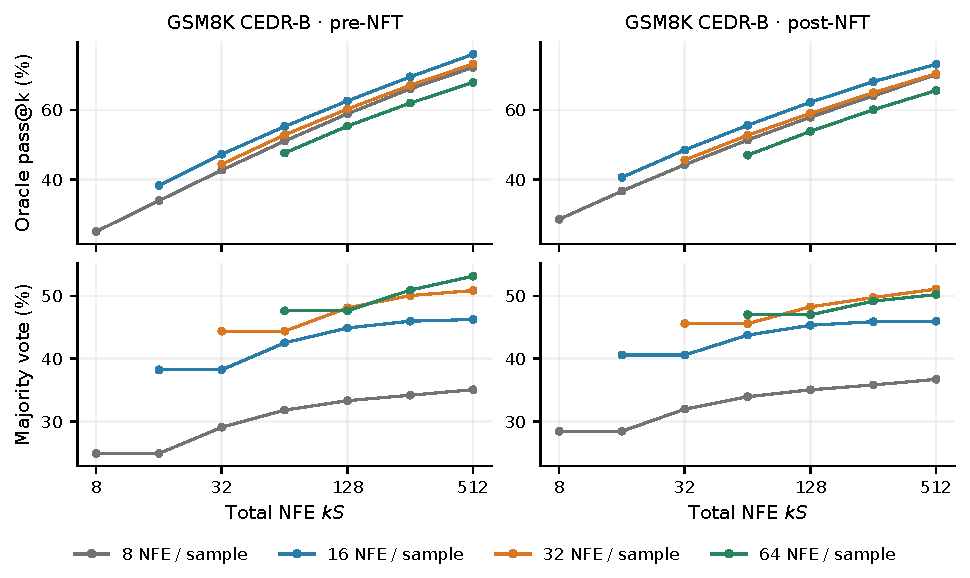
\includegraphics[width=.9\linewidth]{figures/appendix_cedr_b_stages_dmd2.pdf}
\caption{GSM8K CEDR-B before and after NFT with DMD2-style sampling. Upper panels show oracle pass@$k$; lower panels show majority-vote accuracy. Colors denote denoising NFE per sample. The same 64/32/16/8 sample cohorts and total budget of 512 denoising calls are used as in Figure~\ref{fig:headlinestages}. Table~\ref{tab:budgetvaluesgsmb} gives every plotted value with problem-bootstrap SDs.}
\label{fig:elfbstages}
\end{figure}

\FloatBarrier
\subsection{Inference allocation across sampling algorithms}
\label{app:samplerallocations}

Figures~\ref{fig:samplerallocationgsml}--\ref{fig:samplerallocationgsmb} compare ODE, EDM-style index churn ($0.7$), and DMD2-style sampling ($\eta=1$) at the fixed supervised and NFT endpoints. Columns fix denoising NFE per sample; rows separate oracle pass@$k$ and majority voting before and after NFT. The horizontal axis is the total denoising budget $kS$. We use all 64/32/16/8 saved draws at 8/16/32/64 NFE, respectively, up to 512 total calls, with identical ordered seed cohorts across samplers. Clocks remain $(2.5,2,1.5)$; GSM8K uses SCCFG 2 and MATH500 SCCFG 3. Checkpoints, EMA selectors, prompts, scorers, and voting rules match the headline comparisons in Appendix~\ref{app:experimentdetails}. These comparisons include each sampler's integration and terminal-state convention (Appendix~\ref{app:samplerimplementation}).

At 64 NFE, both stochastic samplers improve pass@1 over ODE at all six endpoints, but the ranking can change with the sample count and selection rule. For GSM8K CEDR-L after NFT, eight 64-step draws give ODE pass@8 of 83.02\%, compared with 80.21\% for EDM-style and 80.82\% for DMD2-style sampling. Yet DMD2-style majority voting reaches 71.81\%, versus ODE's 70.58\%. For MATH500 after NFT, the same allocation yields DMD2-style voting accuracy of 38.80\%, versus ODE's 33.38\%; at eight steps and 64 draws, ODE voting instead reaches 28.63\%, versus 27.80\% for DMD2-style sampling. Thus improvements in single-sample accuracy do not imply uniform improvements in oracle coverage or voting at every allocation. Our headline sampler remains fixed across all budgets.

\begin{figure}[p]
\centering
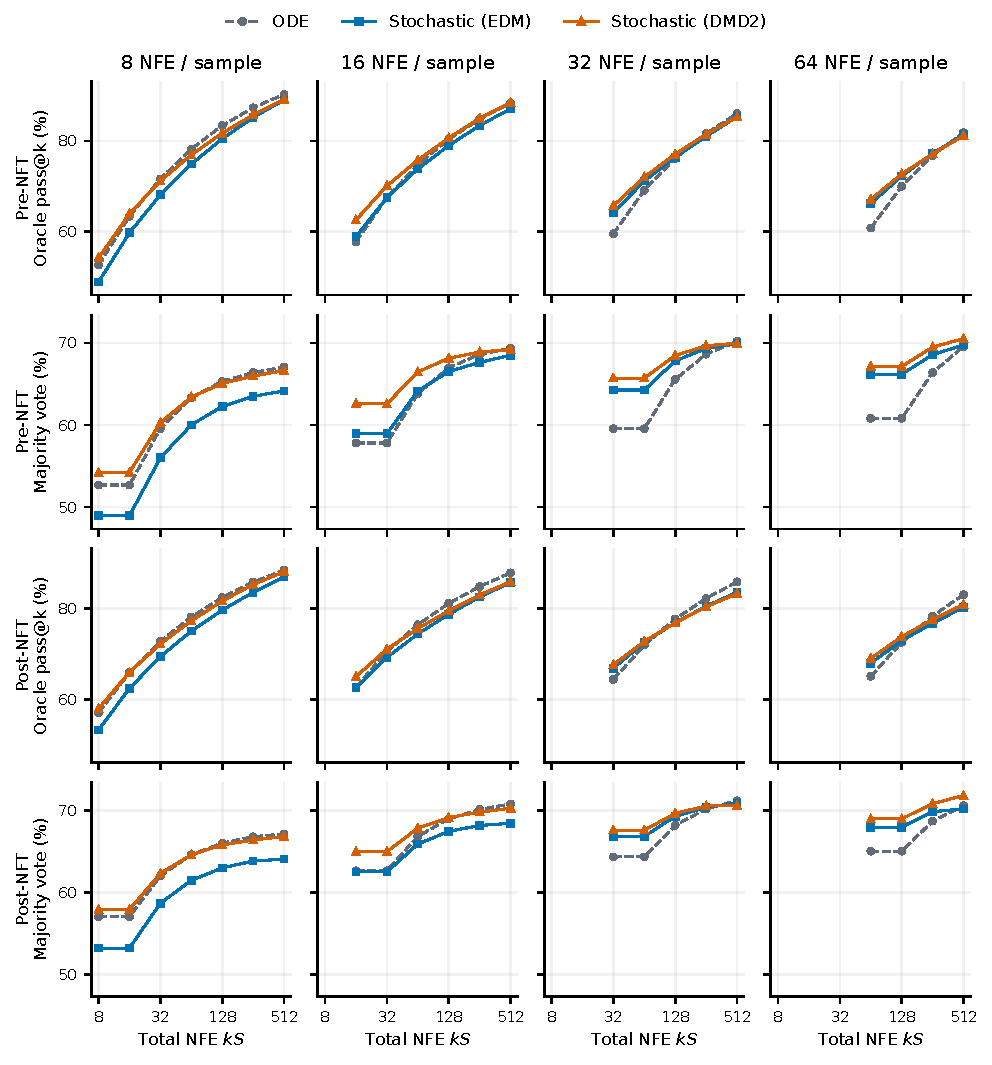
\includegraphics[width=\linewidth]{figures/appendix_sampler_allocation_gsm_l.pdf}
\caption{\textbf{GSM8K, CEDR-L: inference allocation across samplers.} Pre-NFT is epoch 21; post-NFT is NFT update 600. Columns fix NFE per sample; rows show pre-/post-NFT oracle and majority-vote accuracy. Colors and markers distinguish samplers; axes match across samplers and training stages within each metric. Numerical values and uncertainty: Tables~\ref{tab:samplerbudgetgsmlode}--\ref{tab:samplerbudgetgsmledm} for ODE/EDM, and Table~\ref{tab:budgetvaluesgsml} for DMD2.}
\label{fig:samplerallocationgsml}
\end{figure}

\begin{figure}[p]
\centering
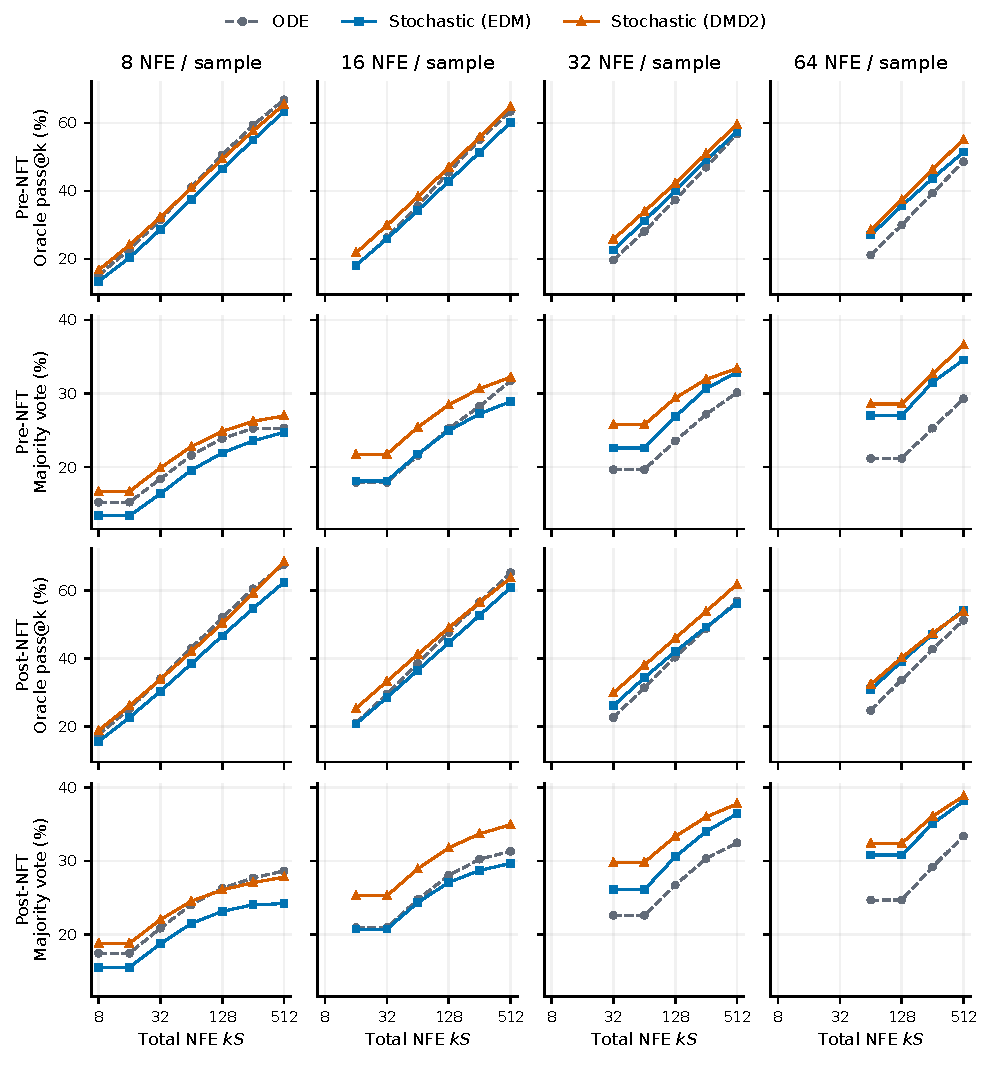
\includegraphics[width=\linewidth]{figures/appendix_sampler_allocation_math_l.pdf}
\caption{\textbf{MATH500, CEDR-L: inference allocation across samplers.} Pre-NFT is epoch 21; post-NFT is NFT update 600. Columns fix NFE per sample; rows show pre-/post-NFT oracle and majority-vote accuracy. Colors and markers distinguish samplers; axes match across samplers and training stages within each metric. Numerical values and uncertainty: Tables~\ref{tab:samplerbudgetmathlode}--\ref{tab:samplerbudgetmathledm} for ODE/EDM, and Table~\ref{tab:budgetvaluesmathl} for DMD2.}
\label{fig:samplerallocationmathl}
\end{figure}

\begin{figure}[p]
\centering
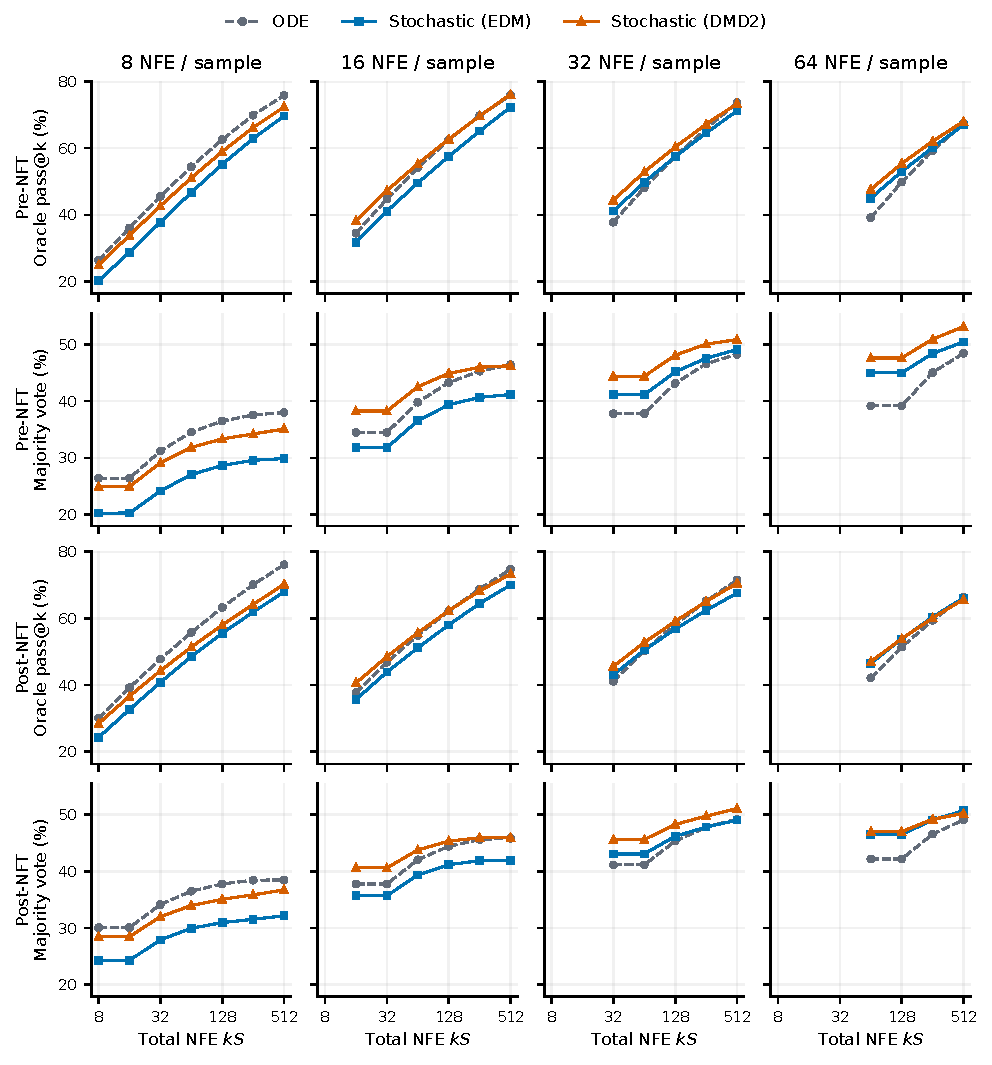
\includegraphics[width=\linewidth]{figures/appendix_sampler_allocation_gsm_b.pdf}
\caption{\textbf{GSM8K, CEDR-B: inference allocation across samplers.} Pre-NFT is epoch 18; post-NFT is NFT update 300. Columns fix NFE per sample; rows show pre-/post-NFT oracle and majority-vote accuracy. Colors and markers distinguish samplers; axes match across samplers and training stages within each metric. Numerical values and uncertainty: Tables~\ref{tab:samplerbudgetgsmbode}--\ref{tab:samplerbudgetgsmbedm} for ODE/EDM, and Table~\ref{tab:budgetvaluesgsmb} for DMD2.}
\label{fig:samplerallocationgsmb}
\end{figure}

\FloatBarrier
\subsection{Numerical inference-allocation results}
\label{app:budgetvalues}

Tables~\ref{tab:budgetvaluesgsml}--\ref{tab:budgetvaluesgsmb} give every oracle and voting point in Figures~\ref{fig:headlinestages} and~\ref{fig:elfbstages}, using DMD2-style sampling and SCCFG 2 for GSM8K / 3 for MATH500. Each table pairs supervised and NFT checkpoints at identical denoising depths, sample counts, and ordered generation seeds. The underlying populations contain all 1,319 GSM8K or 500 MATH500 test problems.

Metrics and uncertainty are defined in Appendix~\ref{app:experimentdetails}.

\paragraph{Paired NFT improvements.}
For DMD2-style sampling at 64 steps, NFT changes CEDR-L pass@1 by $+1.84$ points ($[+0.99,+2.69]$) on GSM8K and $+3.83$ points ($[+2.18,+5.40]$) on MATH500. The corresponding CEDR-B change is $-0.63$ points ($[-1.60,+0.34]$). At 64 steps and eight samples, MATH500 oracle accuracy changes by $-1.40$ points ($[-4.80,+2.00]$) and voting by $+2.23$ points ($[-0.32,+4.79]$). These are paired 95\% problem-bootstrap intervals conditional on the fixed checkpoints and draws; they do not include training or sampler-selection uncertainty.

\paragraph{Interpreting NFT gains across allocations.}
At eight steps on GSM8K CEDR-L, NFT raises pass@1 from 54.23\% to 57.93\%, while pass@64 changes from 89.16\% to 88.02\%. On MATH500 at the same allocation, oracle accuracy rises from 65.40\% to 68.40\% and voting from 26.95\% to 27.80\%. Thus oracle and voting improvements both depend on the allocation. For independent draws with problem-specific success probability $p_i$, oracle success is $1-(1-p_i)^k$, so gains saturate on problems already solved frequently. Voting instead depends on the correct answer's frequency relative to competing answer groups. Changes in correctness probability, its distribution across problems, and answer-group frequencies can affect these metrics differently; the curves do not alone establish a loss of reasoning diversity.

\begin{table}[!htbp]
\caption{GSM8K, CEDR-L: every point in Figure~\ref{fig:headlinestages}, with DMD2-style sampling and SCCFG 2. Entries are accuracy percentages with problem-bootstrap SDs in parentheses, not across-seed SDs (Appendix~\ref{app:uncertainty}). Each denoising depth uses $n=512/S$ saved draws per problem; $k$-subset averaging uses all $n$.}
\label{tab:budgetvaluesgsml}
\centering\small
\setlength{\tabcolsep}{5pt}
\begin{tabular}{@{}rrr rrrr@{}}
\toprule
& & & \multicolumn{2}{c}{Oracle pass@$k$} & \multicolumn{2}{c}{Majority vote} \\
\cmidrule(lr){4-5}\cmidrule(l){6-7}
NFE $S$ & $k$ & $kS$ & Pre-NFT & Post-NFT & Pre-NFT & Post-NFT \\
\midrule
8 & 1 & 8 & 54.23 {\scriptsize (1.07)} & 57.93 {\scriptsize (1.12)} & 54.23 {\scriptsize (1.07)} & 57.93 {\scriptsize (1.12)} \\
8 & 2 & 16 & 63.92 {\scriptsize (1.10)} & 65.91 {\scriptsize (1.11)} & 54.23 {\scriptsize (1.07)} & 57.93 {\scriptsize (1.12)} \\
8 & 4 & 32 & 71.18 {\scriptsize (1.07)} & 72.13 {\scriptsize (1.08)} & 60.29 {\scriptsize (1.16)} & 62.32 {\scriptsize (1.18)} \\
8 & 8 & 64 & 76.92 {\scriptsize (1.01)} & 77.22 {\scriptsize (1.02)} & 63.41 {\scriptsize (1.19)} & 64.60 {\scriptsize (1.21)} \\
8 & 16 & 128 & 81.67 {\scriptsize (0.95)} & 81.60 {\scriptsize (0.96)} & 65.07 {\scriptsize (1.22)} & 65.80 {\scriptsize (1.23)} \\
8 & 32 & 256 & 85.72 {\scriptsize (0.89)} & 85.23 {\scriptsize (0.92)} & 65.97 {\scriptsize (1.25)} & 66.40 {\scriptsize (1.25)} \\
8 & 64 & 512 & 89.16 {\scriptsize (0.86)} & 88.02 {\scriptsize (0.90)} & 66.64 {\scriptsize (1.29)} & 66.82 {\scriptsize (1.28)} \\
\midrule
16 & 1 & 16 & 62.57 {\scriptsize (1.11)} & 64.96 {\scriptsize (1.14)} & 62.57 {\scriptsize (1.11)} & 64.96 {\scriptsize (1.14)} \\
16 & 2 & 32 & 70.10 {\scriptsize (1.09)} & 71.00 {\scriptsize (1.12)} & 62.58 {\scriptsize (1.11)} & 64.96 {\scriptsize (1.14)} \\
16 & 4 & 64 & 75.76 {\scriptsize (1.03)} & 75.56 {\scriptsize (1.07)} & 66.46 {\scriptsize (1.16)} & 67.83 {\scriptsize (1.19)} \\
16 & 8 & 128 & 80.63 {\scriptsize (0.96)} & 79.42 {\scriptsize (1.02)} & 68.15 {\scriptsize (1.19)} & 69.12 {\scriptsize (1.21)} \\
16 & 16 & 256 & 84.97 {\scriptsize (0.90)} & 82.91 {\scriptsize (0.97)} & 68.90 {\scriptsize (1.21)} & 69.79 {\scriptsize (1.22)} \\
16 & 32 & 512 & 88.40 {\scriptsize (0.88)} & 85.82 {\scriptsize (0.96)} & 69.19 {\scriptsize (1.26)} & 70.27 {\scriptsize (1.25)} \\
\midrule
32 & 1 & 32 & 65.71 {\scriptsize (1.13)} & 67.59 {\scriptsize (1.15)} & 65.71 {\scriptsize (1.13)} & 67.59 {\scriptsize (1.15)} \\
32 & 2 & 64 & 72.04 {\scriptsize (1.09)} & 72.72 {\scriptsize (1.12)} & 65.71 {\scriptsize (1.13)} & 67.59 {\scriptsize (1.15)} \\
32 & 4 & 128 & 77.06 {\scriptsize (1.05)} & 76.79 {\scriptsize (1.08)} & 68.47 {\scriptsize (1.17)} & 69.62 {\scriptsize (1.19)} \\
32 & 8 & 256 & 81.47 {\scriptsize (1.00)} & 80.31 {\scriptsize (1.04)} & 69.65 {\scriptsize (1.19)} & 70.54 {\scriptsize (1.22)} \\
32 & 16 & 512 & 85.22 {\scriptsize (0.99)} & 83.24 {\scriptsize (1.04)} & 69.97 {\scriptsize (1.24)} & 70.58 {\scriptsize (1.26)} \\
\midrule
64 & 1 & 64 & 67.13 {\scriptsize (1.15)} & 68.97 {\scriptsize (1.16)} & 67.13 {\scriptsize (1.15)} & 68.97 {\scriptsize (1.16)} \\
64 & 2 & 128 & 72.71 {\scriptsize (1.12)} & 73.76 {\scriptsize (1.13)} & 67.13 {\scriptsize (1.15)} & 68.97 {\scriptsize (1.16)} \\
64 & 4 & 256 & 77.12 {\scriptsize (1.09)} & 77.55 {\scriptsize (1.10)} & 69.50 {\scriptsize (1.19)} & 70.82 {\scriptsize (1.20)} \\
64 & 8 & 512 & 81.12 {\scriptsize (1.09)} & 80.82 {\scriptsize (1.09)} & 70.52 {\scriptsize (1.24)} & 71.81 {\scriptsize (1.24)} \\
\bottomrule
\end{tabular}
\end{table}
\begin{table}[!htbp]
\caption{MATH500, CEDR-L: every point in Figure~\ref{fig:headlinestages}, with DMD2-style sampling and SCCFG 3. Entries are accuracy percentages with problem-bootstrap SDs in parentheses, not across-seed SDs (Appendix~\ref{app:uncertainty}). Each denoising depth uses $n=512/S$ saved draws per problem; $k$-subset averaging uses all $n$.}
\label{tab:budgetvaluesmathl}
\centering\small
\setlength{\tabcolsep}{5pt}
\begin{tabular}{@{}rrr rrrr@{}}
\toprule
& & & \multicolumn{2}{c}{Oracle pass@$k$} & \multicolumn{2}{c}{Majority vote} \\
\cmidrule(lr){4-5}\cmidrule(l){6-7}
NFE $S$ & $k$ & $kS$ & Pre-NFT & Post-NFT & Pre-NFT & Post-NFT \\
\midrule
8 & 1 & 8 & 16.70 {\scriptsize (1.16)} & 18.82 {\scriptsize (1.28)} & 16.70 {\scriptsize (1.16)} & 18.82 {\scriptsize (1.28)} \\
8 & 2 & 16 & 24.07 {\scriptsize (1.45)} & 26.06 {\scriptsize (1.54)} & 16.71 {\scriptsize (1.16)} & 18.82 {\scriptsize (1.28)} \\
8 & 4 & 32 & 32.28 {\scriptsize (1.67)} & 33.83 {\scriptsize (1.72)} & 19.89 {\scriptsize (1.40)} & 22.02 {\scriptsize (1.52)} \\
8 & 8 & 64 & 40.83 {\scriptsize (1.82)} & 41.96 {\scriptsize (1.84)} & 22.79 {\scriptsize (1.57)} & 24.53 {\scriptsize (1.66)} \\
8 & 16 & 128 & 49.38 {\scriptsize (1.92)} & 50.34 {\scriptsize (1.90)} & 24.85 {\scriptsize (1.69)} & 26.05 {\scriptsize (1.77)} \\
8 & 32 & 256 & 57.64 {\scriptsize (1.99)} & 59.14 {\scriptsize (1.94)} & 26.22 {\scriptsize (1.81)} & 27.05 {\scriptsize (1.86)} \\
8 & 64 & 512 & 65.40 {\scriptsize (2.12)} & 68.40 {\scriptsize (2.08)} & 26.95 {\scriptsize (1.98)} & 27.80 {\scriptsize (2.00)} \\
\midrule
16 & 1 & 16 & 21.75 {\scriptsize (1.37)} & 25.26 {\scriptsize (1.51)} & 21.75 {\scriptsize (1.37)} & 25.26 {\scriptsize (1.51)} \\
16 & 2 & 32 & 29.87 {\scriptsize (1.63)} & 33.25 {\scriptsize (1.74)} & 21.75 {\scriptsize (1.37)} & 25.26 {\scriptsize (1.51)} \\
16 & 4 & 64 & 38.30 {\scriptsize (1.80)} & 41.18 {\scriptsize (1.87)} & 25.41 {\scriptsize (1.61)} & 28.92 {\scriptsize (1.73)} \\
16 & 8 & 128 & 46.93 {\scriptsize (1.90)} & 48.98 {\scriptsize (1.96)} & 28.44 {\scriptsize (1.77)} & 31.78 {\scriptsize (1.87)} \\
16 & 16 & 256 & 55.81 {\scriptsize (1.99)} & 56.46 {\scriptsize (2.03)} & 30.65 {\scriptsize (1.90)} & 33.68 {\scriptsize (1.98)} \\
16 & 32 & 512 & 64.80 {\scriptsize (2.14)} & 63.60 {\scriptsize (2.16)} & 32.21 {\scriptsize (2.07)} & 34.93 {\scriptsize (2.11)} \\
\midrule
32 & 1 & 32 & 25.76 {\scriptsize (1.54)} & 29.80 {\scriptsize (1.65)} & 25.76 {\scriptsize (1.54)} & 29.80 {\scriptsize (1.65)} \\
32 & 2 & 64 & 33.90 {\scriptsize (1.74)} & 37.89 {\scriptsize (1.82)} & 25.76 {\scriptsize (1.54)} & 29.80 {\scriptsize (1.65)} \\
32 & 4 & 128 & 42.27 {\scriptsize (1.87)} & 45.91 {\scriptsize (1.94)} & 29.38 {\scriptsize (1.76)} & 33.32 {\scriptsize (1.84)} \\
32 & 8 & 256 & 50.98 {\scriptsize (2.00)} & 53.80 {\scriptsize (2.03)} & 31.92 {\scriptsize (1.90)} & 35.97 {\scriptsize (1.96)} \\
32 & 16 & 512 & 59.60 {\scriptsize (2.20)} & 61.80 {\scriptsize (2.19)} & 33.39 {\scriptsize (2.07)} & 37.74 {\scriptsize (2.13)} \\
\midrule
64 & 1 & 64 & 28.58 {\scriptsize (1.60)} & 32.40 {\scriptsize (1.76)} & 28.58 {\scriptsize (1.60)} & 32.40 {\scriptsize (1.76)} \\
64 & 2 & 128 & 37.39 {\scriptsize (1.82)} & 40.20 {\scriptsize (1.92)} & 28.58 {\scriptsize (1.60)} & 32.40 {\scriptsize (1.76)} \\
64 & 4 & 256 & 46.28 {\scriptsize (1.99)} & 47.41 {\scriptsize (2.06)} & 32.65 {\scriptsize (1.84)} & 36.07 {\scriptsize (1.94)} \\
64 & 8 & 512 & 55.20 {\scriptsize (2.24)} & 53.80 {\scriptsize (2.24)} & 36.58 {\scriptsize (2.09)} & 38.80 {\scriptsize (2.13)} \\
\bottomrule
\end{tabular}
\end{table}
\begin{table}[!htbp]
\caption{GSM8K, CEDR-B: every point in Figure~\ref{fig:elfbstages}, with DMD2-style sampling and SCCFG 2. Entries are accuracy percentages with problem-bootstrap SDs in parentheses, not across-seed SDs (Appendix~\ref{app:uncertainty}). Each denoising depth uses $n=512/S$ saved draws per problem; $k$-subset averaging uses all $n$.}
\label{tab:budgetvaluesgsmb}
\centering\small
\setlength{\tabcolsep}{5pt}
\begin{tabular}{@{}rrr rrrr@{}}
\toprule
& & & \multicolumn{2}{c}{Oracle pass@$k$} & \multicolumn{2}{c}{Majority vote} \\
\cmidrule(lr){4-5}\cmidrule(l){6-7}
NFE $S$ & $k$ & $kS$ & Pre-NFT & Post-NFT & Pre-NFT & Post-NFT \\
\midrule
8 & 1 & 8 & 24.95 {\scriptsize (0.87)} & 28.48 {\scriptsize (0.96)} & 24.95 {\scriptsize (0.87)} & 28.48 {\scriptsize (0.96)} \\
8 & 2 & 16 & 33.86 {\scriptsize (1.02)} & 36.63 {\scriptsize (1.08)} & 24.95 {\scriptsize (0.87)} & 28.48 {\scriptsize (0.96)} \\
8 & 4 & 32 & 42.68 {\scriptsize (1.12)} & 44.26 {\scriptsize (1.16)} & 29.12 {\scriptsize (1.02)} & 32.00 {\scriptsize (1.08)} \\
8 & 8 & 64 & 51.08 {\scriptsize (1.17)} & 51.36 {\scriptsize (1.20)} & 31.84 {\scriptsize (1.11)} & 33.96 {\scriptsize (1.15)} \\
8 & 16 & 128 & 58.93 {\scriptsize (1.18)} & 57.95 {\scriptsize (1.21)} & 33.34 {\scriptsize (1.17)} & 35.06 {\scriptsize (1.20)} \\
8 & 32 & 256 & 66.15 {\scriptsize (1.19)} & 64.13 {\scriptsize (1.22)} & 34.21 {\scriptsize (1.23)} & 35.84 {\scriptsize (1.25)} \\
8 & 64 & 512 & 72.33 {\scriptsize (1.22)} & 70.20 {\scriptsize (1.25)} & 35.09 {\scriptsize (1.31)} & 36.73 {\scriptsize (1.31)} \\
\midrule
16 & 1 & 16 & 38.25 {\scriptsize (1.05)} & 40.60 {\scriptsize (1.10)} & 38.25 {\scriptsize (1.05)} & 40.60 {\scriptsize (1.10)} \\
16 & 2 & 32 & 47.26 {\scriptsize (1.14)} & 48.50 {\scriptsize (1.17)} & 38.25 {\scriptsize (1.05)} & 40.60 {\scriptsize (1.10)} \\
16 & 4 & 64 & 55.29 {\scriptsize (1.16)} & 55.64 {\scriptsize (1.18)} & 42.54 {\scriptsize (1.17)} & 43.76 {\scriptsize (1.20)} \\
16 & 8 & 128 & 62.65 {\scriptsize (1.16)} & 62.27 {\scriptsize (1.19)} & 44.90 {\scriptsize (1.23)} & 45.33 {\scriptsize (1.25)} \\
16 & 16 & 256 & 69.60 {\scriptsize (1.15)} & 68.20 {\scriptsize (1.19)} & 45.97 {\scriptsize (1.28)} & 45.90 {\scriptsize (1.29)} \\
16 & 32 & 512 & 76.12 {\scriptsize (1.18)} & 73.24 {\scriptsize (1.23)} & 46.25 {\scriptsize (1.36)} & 45.97 {\scriptsize (1.35)} \\
\midrule
32 & 1 & 32 & 44.39 {\scriptsize (1.11)} & 45.59 {\scriptsize (1.16)} & 44.39 {\scriptsize (1.11)} & 45.59 {\scriptsize (1.16)} \\
32 & 2 & 64 & 52.86 {\scriptsize (1.17)} & 52.74 {\scriptsize (1.20)} & 44.39 {\scriptsize (1.11)} & 45.59 {\scriptsize (1.16)} \\
32 & 4 & 128 & 60.30 {\scriptsize (1.18)} & 59.07 {\scriptsize (1.21)} & 48.10 {\scriptsize (1.21)} & 48.26 {\scriptsize (1.24)} \\
32 & 8 & 256 & 67.16 {\scriptsize (1.18)} & 65.01 {\scriptsize (1.22)} & 50.05 {\scriptsize (1.27)} & 49.73 {\scriptsize (1.29)} \\
32 & 16 & 512 & 73.31 {\scriptsize (1.22)} & 70.51 {\scriptsize (1.26)} & 50.85 {\scriptsize (1.35)} & 51.08 {\scriptsize (1.36)} \\
\midrule
64 & 1 & 64 & 47.62 {\scriptsize (1.16)} & 47.00 {\scriptsize (1.19)} & 47.62 {\scriptsize (1.16)} & 47.00 {\scriptsize (1.19)} \\
64 & 2 & 128 & 55.39 {\scriptsize (1.21)} & 53.86 {\scriptsize (1.23)} & 47.62 {\scriptsize (1.16)} & 47.00 {\scriptsize (1.19)} \\
64 & 4 & 256 & 62.04 {\scriptsize (1.23)} & 60.11 {\scriptsize (1.26)} & 50.92 {\scriptsize (1.26)} & 49.17 {\scriptsize (1.27)} \\
64 & 8 & 512 & 68.01 {\scriptsize (1.28)} & 65.66 {\scriptsize (1.32)} & 53.13 {\scriptsize (1.34)} & 50.21 {\scriptsize (1.36)} \\
\bottomrule
\end{tabular}
\end{table}

\FloatBarrier
\subsubsection{Numerical values for the other samplers}
\label{app:samplerbudgetvalues}
Tables~\ref{tab:samplerbudgetgsmlode}--\ref{tab:samplerbudgetgsmbedm} give every ODE and EDM-style point in Figures~\ref{fig:samplerallocationgsml}--\ref{fig:samplerallocationgsmb}. The DMD2-style values are already listed in Tables~\ref{tab:budgetvaluesgsml}--\ref{tab:budgetvaluesgsmb}. Parentheses report problem-bootstrap standard errors, with the same 4,000-replicate procedure and seed as the headline tables (Appendix~\ref{app:uncertainty}). All comparisons use the full benchmark and every saved draw at each NFE.

\begin{table}[p]
\centering\small
\setlength{\tabcolsep}{5pt}
\caption{GSM8K, CEDR-L: ODE values in Figure~\ref{fig:samplerallocationgsml}. Entries are accuracy percentages, with problem-bootstrap standard errors in parentheses (Appendix~\ref{app:uncertainty}). SCCFG 2; asynchronous clocks $(2.5,2,1.5)$.}
\label{tab:samplerbudgetgsmlode}
\begin{tabular}{@{}rrr rrrr@{}}
\toprule
& & & \multicolumn{2}{c}{Oracle pass@$k$} & \multicolumn{2}{c}{Majority vote} \\
\cmidrule(lr){4-5}\cmidrule(l){6-7}
NFE $S$ & $k$ & $kS$ & Pre-NFT & Post-NFT & Pre-NFT & Post-NFT \\
\midrule
8 & 1 & 8 & 52.69 {\scriptsize (1.04)} & 57.06 {\scriptsize (1.09)} & 52.69 {\scriptsize (1.04)} & 57.06 {\scriptsize (1.09)} \\
8 & 2 & 16 & 63.43 {\scriptsize (1.07)} & 65.89 {\scriptsize (1.09)} & 52.69 {\scriptsize (1.04)} & 57.06 {\scriptsize (1.09)} \\
8 & 4 & 32 & 71.64 {\scriptsize (1.03)} & 72.71 {\scriptsize (1.05)} & 59.57 {\scriptsize (1.14)} & 62.02 {\scriptsize (1.16)} \\
8 & 8 & 64 & 78.18 {\scriptsize (0.96)} & 78.11 {\scriptsize (1.00)} & 63.32 {\scriptsize (1.17)} & 64.61 {\scriptsize (1.19)} \\
8 & 16 & 128 & 83.35 {\scriptsize (0.90)} & 82.37 {\scriptsize (0.94)} & 65.32 {\scriptsize (1.20)} & 66.01 {\scriptsize (1.21)} \\
8 & 32 & 256 & 87.28 {\scriptsize (0.83)} & 85.75 {\scriptsize (0.89)} & 66.40 {\scriptsize (1.23)} & 66.78 {\scriptsize (1.24)} \\
8 & 64 & 512 & 90.22 {\scriptsize (0.81)} & 88.40 {\scriptsize (0.88)} & 67.06 {\scriptsize (1.28)} & 67.13 {\scriptsize (1.30)} \\
\midrule
16 & 1 & 16 & 57.80 {\scriptsize (1.07)} & 62.64 {\scriptsize (1.10)} & 57.80 {\scriptsize (1.07)} & 62.64 {\scriptsize (1.10)} \\
16 & 2 & 32 & 67.50 {\scriptsize (1.07)} & 70.46 {\scriptsize (1.08)} & 57.80 {\scriptsize (1.07)} & 62.64 {\scriptsize (1.10)} \\
16 & 4 & 64 & 74.73 {\scriptsize (1.02)} & 76.40 {\scriptsize (1.02)} & 63.83 {\scriptsize (1.14)} & 66.82 {\scriptsize (1.15)} \\
16 & 8 & 128 & 80.37 {\scriptsize (0.96)} & 81.07 {\scriptsize (0.97)} & 66.97 {\scriptsize (1.17)} & 68.98 {\scriptsize (1.17)} \\
16 & 16 & 256 & 84.78 {\scriptsize (0.91)} & 84.78 {\scriptsize (0.92)} & 68.62 {\scriptsize (1.19)} & 70.11 {\scriptsize (1.20)} \\
16 & 32 & 512 & 88.32 {\scriptsize (0.89)} & 87.79 {\scriptsize (0.91)} & 69.34 {\scriptsize (1.25)} & 70.79 {\scriptsize (1.24)} \\
\midrule
32 & 1 & 32 & 59.55 {\scriptsize (1.08)} & 64.33 {\scriptsize (1.10)} & 59.55 {\scriptsize (1.08)} & 64.33 {\scriptsize (1.10)} \\
32 & 2 & 64 & 69.14 {\scriptsize (1.07)} & 71.93 {\scriptsize (1.08)} & 59.55 {\scriptsize (1.08)} & 64.33 {\scriptsize (1.10)} \\
32 & 4 & 128 & 76.16 {\scriptsize (1.02)} & 77.67 {\scriptsize (1.03)} & 65.57 {\scriptsize (1.15)} & 68.18 {\scriptsize (1.15)} \\
32 & 8 & 256 & 81.61 {\scriptsize (0.97)} & 82.19 {\scriptsize (0.98)} & 68.62 {\scriptsize (1.18)} & 70.18 {\scriptsize (1.18)} \\
32 & 16 & 512 & 85.97 {\scriptsize (0.95)} & 85.82 {\scriptsize (0.97)} & 70.21 {\scriptsize (1.24)} & 71.18 {\scriptsize (1.25)} \\
\midrule
64 & 1 & 64 & 60.81 {\scriptsize (1.10)} & 65.03 {\scriptsize (1.12)} & 60.81 {\scriptsize (1.10)} & 65.03 {\scriptsize (1.12)} \\
64 & 2 & 128 & 69.99 {\scriptsize (1.09)} & 72.50 {\scriptsize (1.08)} & 60.81 {\scriptsize (1.10)} & 65.03 {\scriptsize (1.12)} \\
64 & 4 & 256 & 76.77 {\scriptsize (1.06)} & 78.27 {\scriptsize (1.04)} & 66.40 {\scriptsize (1.17)} & 68.69 {\scriptsize (1.17)} \\
64 & 8 & 512 & 81.80 {\scriptsize (1.06)} & 83.02 {\scriptsize (1.04)} & 69.56 {\scriptsize (1.24)} & 70.58 {\scriptsize (1.23)} \\
\bottomrule
\end{tabular}
\end{table}

\begin{table}[p]
\centering\small
\setlength{\tabcolsep}{5pt}
\caption{GSM8K, CEDR-L: Stochastic (EDM) values in Figure~\ref{fig:samplerallocationgsml}. Entries are accuracy percentages, with problem-bootstrap standard errors in parentheses (Appendix~\ref{app:uncertainty}). SCCFG 2; asynchronous clocks $(2.5,2,1.5)$.}
\label{tab:samplerbudgetgsmledm}
\begin{tabular}{@{}rrr rrrr@{}}
\toprule
& & & \multicolumn{2}{c}{Oracle pass@$k$} & \multicolumn{2}{c}{Majority vote} \\
\cmidrule(lr){4-5}\cmidrule(l){6-7}
NFE $S$ & $k$ & $kS$ & Pre-NFT & Post-NFT & Pre-NFT & Post-NFT \\
\midrule
8 & 1 & 8 & 48.95 {\scriptsize (1.04)} & 53.22 {\scriptsize (1.09)} & 48.95 {\scriptsize (1.04)} & 53.22 {\scriptsize (1.09)} \\
8 & 2 & 16 & 59.77 {\scriptsize (1.09)} & 62.39 {\scriptsize (1.12)} & 48.96 {\scriptsize (1.04)} & 53.22 {\scriptsize (1.09)} \\
8 & 4 & 32 & 68.15 {\scriptsize (1.07)} & 69.39 {\scriptsize (1.10)} & 56.01 {\scriptsize (1.15)} & 58.69 {\scriptsize (1.18)} \\
8 & 8 & 64 & 74.88 {\scriptsize (1.02)} & 74.98 {\scriptsize (1.05)} & 60.02 {\scriptsize (1.19)} & 61.48 {\scriptsize (1.21)} \\
8 & 16 & 128 & 80.44 {\scriptsize (0.95)} & 79.60 {\scriptsize (0.99)} & 62.26 {\scriptsize (1.23)} & 62.99 {\scriptsize (1.24)} \\
8 & 32 & 256 & 85.14 {\scriptsize (0.89)} & 83.50 {\scriptsize (0.94)} & 63.50 {\scriptsize (1.26)} & 63.82 {\scriptsize (1.27)} \\
8 & 64 & 512 & 89.01 {\scriptsize (0.86)} & 86.88 {\scriptsize (0.92)} & 64.16 {\scriptsize (1.31)} & 64.06 {\scriptsize (1.32)} \\
\midrule
16 & 1 & 16 & 58.93 {\scriptsize (1.10)} & 62.51 {\scriptsize (1.14)} & 58.93 {\scriptsize (1.10)} & 62.51 {\scriptsize (1.14)} \\
16 & 2 & 32 & 67.52 {\scriptsize (1.10)} & 69.22 {\scriptsize (1.12)} & 58.93 {\scriptsize (1.10)} & 62.51 {\scriptsize (1.14)} \\
16 & 4 & 64 & 73.81 {\scriptsize (1.05)} & 74.34 {\scriptsize (1.08)} & 64.14 {\scriptsize (1.17)} & 65.90 {\scriptsize (1.18)} \\
16 & 8 & 128 & 78.97 {\scriptsize (0.99)} & 78.67 {\scriptsize (1.02)} & 66.51 {\scriptsize (1.19)} & 67.44 {\scriptsize (1.21)} \\
16 & 16 & 256 & 83.38 {\scriptsize (0.94)} & 82.49 {\scriptsize (0.98)} & 67.64 {\scriptsize (1.21)} & 68.16 {\scriptsize (1.24)} \\
16 & 32 & 512 & 87.04 {\scriptsize (0.92)} & 85.67 {\scriptsize (0.97)} & 68.49 {\scriptsize (1.26)} & 68.43 {\scriptsize (1.28)} \\
\midrule
32 & 1 & 32 & 64.27 {\scriptsize (1.12)} & 66.83 {\scriptsize (1.14)} & 64.27 {\scriptsize (1.12)} & 66.83 {\scriptsize (1.14)} \\
32 & 2 & 64 & 71.16 {\scriptsize (1.10)} & 72.49 {\scriptsize (1.11)} & 64.27 {\scriptsize (1.12)} & 66.84 {\scriptsize (1.14)} \\
32 & 4 & 128 & 76.39 {\scriptsize (1.05)} & 76.83 {\scriptsize (1.07)} & 67.80 {\scriptsize (1.17)} & 69.27 {\scriptsize (1.18)} \\
32 & 8 & 256 & 80.97 {\scriptsize (1.00)} & 80.44 {\scriptsize (1.04)} & 69.34 {\scriptsize (1.20)} & 70.37 {\scriptsize (1.20)} \\
32 & 16 & 512 & 85.29 {\scriptsize (0.98)} & 83.55 {\scriptsize (1.03)} & 69.91 {\scriptsize (1.25)} & 70.88 {\scriptsize (1.25)} \\
\midrule
64 & 1 & 64 & 66.20 {\scriptsize (1.14)} & 67.93 {\scriptsize (1.16)} & 66.20 {\scriptsize (1.14)} & 67.93 {\scriptsize (1.16)} \\
64 & 2 & 128 & 72.25 {\scriptsize (1.11)} & 72.87 {\scriptsize (1.14)} & 66.20 {\scriptsize (1.14)} & 67.93 {\scriptsize (1.16)} \\
64 & 4 & 256 & 77.25 {\scriptsize (1.08)} & 76.72 {\scriptsize (1.10)} & 68.56 {\scriptsize (1.18)} & 69.84 {\scriptsize (1.20)} \\
64 & 8 & 512 & 81.35 {\scriptsize (1.08)} & 80.21 {\scriptsize (1.11)} & 69.77 {\scriptsize (1.24)} & 70.18 {\scriptsize (1.25)} \\
\bottomrule
\end{tabular}
\end{table}

\begin{table}[p]
\centering\small
\setlength{\tabcolsep}{5pt}
\caption{MATH500, CEDR-L: ODE values in Figure~\ref{fig:samplerallocationmathl}. Entries are accuracy percentages, with problem-bootstrap standard errors in parentheses (Appendix~\ref{app:uncertainty}). SCCFG 3; asynchronous clocks $(2.5,2,1.5)$.}
\label{tab:samplerbudgetmathlode}
\begin{tabular}{@{}rrr rrrr@{}}
\toprule
& & & \multicolumn{2}{c}{Oracle pass@$k$} & \multicolumn{2}{c}{Majority vote} \\
\cmidrule(lr){4-5}\cmidrule(l){6-7}
NFE $S$ & $k$ & $kS$ & Pre-NFT & Post-NFT & Pre-NFT & Post-NFT \\
\midrule
8 & 1 & 8 & 15.23 {\scriptsize (1.06)} & 17.45 {\scriptsize (1.17)} & 15.23 {\scriptsize (1.06)} & 17.45 {\scriptsize (1.17)} \\
8 & 2 & 16 & 22.75 {\scriptsize (1.35)} & 25.22 {\scriptsize (1.45)} & 15.24 {\scriptsize (1.06)} & 17.46 {\scriptsize (1.17)} \\
8 & 4 & 32 & 31.59 {\scriptsize (1.59)} & 33.93 {\scriptsize (1.67)} & 18.37 {\scriptsize (1.30)} & 20.86 {\scriptsize (1.42)} \\
8 & 8 & 64 & 41.11 {\scriptsize (1.77)} & 43.01 {\scriptsize (1.81)} & 21.58 {\scriptsize (1.49)} & 24.06 {\scriptsize (1.60)} \\
8 & 16 & 128 & 50.60 {\scriptsize (1.90)} & 51.99 {\scriptsize (1.90)} & 23.90 {\scriptsize (1.63)} & 26.30 {\scriptsize (1.73)} \\
8 & 32 & 256 & 59.35 {\scriptsize (1.98)} & 60.44 {\scriptsize (1.98)} & 25.26 {\scriptsize (1.76)} & 27.70 {\scriptsize (1.86)} \\
8 & 64 & 512 & 66.80 {\scriptsize (2.10)} & 67.60 {\scriptsize (2.11)} & 25.30 {\scriptsize (1.92)} & 28.63 {\scriptsize (1.99)} \\
\midrule
16 & 1 & 16 & 17.93 {\scriptsize (1.17)} & 20.93 {\scriptsize (1.31)} & 17.93 {\scriptsize (1.17)} & 20.93 {\scriptsize (1.31)} \\
16 & 2 & 32 & 26.24 {\scriptsize (1.46)} & 29.47 {\scriptsize (1.59)} & 17.93 {\scriptsize (1.17)} & 20.93 {\scriptsize (1.31)} \\
16 & 4 & 64 & 35.64 {\scriptsize (1.69)} & 38.51 {\scriptsize (1.77)} & 21.58 {\scriptsize (1.42)} & 24.77 {\scriptsize (1.57)} \\
16 & 8 & 128 & 45.51 {\scriptsize (1.86)} & 47.61 {\scriptsize (1.88)} & 25.24 {\scriptsize (1.61)} & 28.03 {\scriptsize (1.75)} \\
16 & 16 & 256 & 55.10 {\scriptsize (2.00)} & 56.56 {\scriptsize (1.96)} & 28.26 {\scriptsize (1.78)} & 30.24 {\scriptsize (1.89)} \\
16 & 32 & 512 & 63.40 {\scriptsize (2.17)} & 65.20 {\scriptsize (2.11)} & 31.72 {\scriptsize (2.06)} & 31.30 {\scriptsize (2.07)} \\
\midrule
32 & 1 & 32 & 19.65 {\scriptsize (1.27)} & 22.60 {\scriptsize (1.39)} & 19.65 {\scriptsize (1.27)} & 22.60 {\scriptsize (1.39)} \\
32 & 2 & 64 & 28.09 {\scriptsize (1.57)} & 31.33 {\scriptsize (1.66)} & 19.65 {\scriptsize (1.27)} & 22.61 {\scriptsize (1.39)} \\
32 & 4 & 128 & 37.36 {\scriptsize (1.80)} & 40.33 {\scriptsize (1.87)} & 23.53 {\scriptsize (1.54)} & 26.71 {\scriptsize (1.63)} \\
32 & 8 & 256 & 46.98 {\scriptsize (1.99)} & 48.77 {\scriptsize (2.01)} & 27.18 {\scriptsize (1.76)} & 30.33 {\scriptsize (1.83)} \\
32 & 16 & 512 & 56.80 {\scriptsize (2.24)} & 56.80 {\scriptsize (2.20)} & 30.11 {\scriptsize (2.03)} & 32.45 {\scriptsize (2.06)} \\
\midrule
64 & 1 & 64 & 21.18 {\scriptsize (1.37)} & 24.68 {\scriptsize (1.48)} & 21.18 {\scriptsize (1.37)} & 24.68 {\scriptsize (1.48)} \\
64 & 2 & 128 & 29.99 {\scriptsize (1.68)} & 33.67 {\scriptsize (1.75)} & 21.18 {\scriptsize (1.37)} & 24.69 {\scriptsize (1.48)} \\
64 & 4 & 256 & 39.35 {\scriptsize (1.96)} & 42.73 {\scriptsize (1.97)} & 25.29 {\scriptsize (1.66)} & 29.19 {\scriptsize (1.75)} \\
64 & 8 & 512 & 48.60 {\scriptsize (2.27)} & 51.20 {\scriptsize (2.23)} & 29.28 {\scriptsize (2.00)} & 33.38 {\scriptsize (2.04)} \\
\bottomrule
\end{tabular}
\end{table}

\begin{table}[p]
\centering\small
\setlength{\tabcolsep}{5pt}
\caption{MATH500, CEDR-L: Stochastic (EDM) values in Figure~\ref{fig:samplerallocationmathl}. Entries are accuracy percentages, with problem-bootstrap standard errors in parentheses (Appendix~\ref{app:uncertainty}). SCCFG 3; asynchronous clocks $(2.5,2,1.5)$.}
\label{tab:samplerbudgetmathledm}
\begin{tabular}{@{}rrr rrrr@{}}
\toprule
& & & \multicolumn{2}{c}{Oracle pass@$k$} & \multicolumn{2}{c}{Majority vote} \\
\cmidrule(lr){4-5}\cmidrule(l){6-7}
NFE $S$ & $k$ & $kS$ & Pre-NFT & Post-NFT & Pre-NFT & Post-NFT \\
\midrule
8 & 1 & 8 & 13.38 {\scriptsize (0.97)} & 15.55 {\scriptsize (1.12)} & 13.38 {\scriptsize (0.97)} & 15.55 {\scriptsize (1.12)} \\
8 & 2 & 16 & 20.37 {\scriptsize (1.28)} & 22.61 {\scriptsize (1.42)} & 13.39 {\scriptsize (0.97)} & 15.56 {\scriptsize (1.12)} \\
8 & 4 & 32 & 28.66 {\scriptsize (1.55)} & 30.32 {\scriptsize (1.64)} & 16.37 {\scriptsize (1.22)} & 18.75 {\scriptsize (1.38)} \\
8 & 8 & 64 & 37.58 {\scriptsize (1.76)} & 38.40 {\scriptsize (1.81)} & 19.58 {\scriptsize (1.42)} & 21.49 {\scriptsize (1.56)} \\
8 & 16 & 128 & 46.43 {\scriptsize (1.90)} & 46.60 {\scriptsize (1.93)} & 21.92 {\scriptsize (1.57)} & 23.15 {\scriptsize (1.69)} \\
8 & 32 & 256 & 54.95 {\scriptsize (2.00)} & 54.65 {\scriptsize (2.03)} & 23.57 {\scriptsize (1.71)} & 24.04 {\scriptsize (1.79)} \\
8 & 64 & 512 & 63.40 {\scriptsize (2.16)} & 62.40 {\scriptsize (2.19)} & 24.72 {\scriptsize (1.88)} & 24.20 {\scriptsize (1.91)} \\
\midrule
16 & 1 & 16 & 18.11 {\scriptsize (1.22)} & 20.73 {\scriptsize (1.34)} & 18.11 {\scriptsize (1.22)} & 20.73 {\scriptsize (1.34)} \\
16 & 2 & 32 & 25.88 {\scriptsize (1.52)} & 28.48 {\scriptsize (1.61)} & 18.11 {\scriptsize (1.22)} & 20.73 {\scriptsize (1.34)} \\
16 & 4 & 64 & 34.25 {\scriptsize (1.75)} & 36.51 {\scriptsize (1.79)} & 21.77 {\scriptsize (1.49)} & 24.35 {\scriptsize (1.59)} \\
16 & 8 & 128 & 42.84 {\scriptsize (1.91)} & 44.59 {\scriptsize (1.91)} & 24.94 {\scriptsize (1.67)} & 27.08 {\scriptsize (1.74)} \\
16 & 16 & 256 & 51.38 {\scriptsize (2.03)} & 52.65 {\scriptsize (2.02)} & 27.24 {\scriptsize (1.82)} & 28.71 {\scriptsize (1.85)} \\
16 & 32 & 512 & 60.20 {\scriptsize (2.21)} & 60.80 {\scriptsize (2.20)} & 28.89 {\scriptsize (2.02)} & 29.66 {\scriptsize (2.01)} \\
\midrule
32 & 1 & 32 & 22.60 {\scriptsize (1.39)} & 26.08 {\scriptsize (1.54)} & 22.60 {\scriptsize (1.39)} & 26.08 {\scriptsize (1.54)} \\
32 & 2 & 64 & 31.14 {\scriptsize (1.65)} & 34.29 {\scriptsize (1.78)} & 22.60 {\scriptsize (1.39)} & 26.08 {\scriptsize (1.54)} \\
32 & 4 & 128 & 40.10 {\scriptsize (1.84)} & 41.99 {\scriptsize (1.93)} & 26.84 {\scriptsize (1.65)} & 30.56 {\scriptsize (1.79)} \\
32 & 8 & 256 & 49.05 {\scriptsize (2.00)} & 49.18 {\scriptsize (2.03)} & 30.66 {\scriptsize (1.84)} & 33.99 {\scriptsize (1.95)} \\
32 & 16 & 512 & 57.40 {\scriptsize (2.20)} & 56.20 {\scriptsize (2.20)} & 32.89 {\scriptsize (2.04)} & 36.40 {\scriptsize (2.14)} \\
\midrule
64 & 1 & 64 & 27.00 {\scriptsize (1.57)} & 30.80 {\scriptsize (1.70)} & 27.00 {\scriptsize (1.57)} & 30.80 {\scriptsize (1.70)} \\
64 & 2 & 128 & 35.56 {\scriptsize (1.82)} & 39.12 {\scriptsize (1.89)} & 27.00 {\scriptsize (1.57)} & 30.80 {\scriptsize (1.70)} \\
64 & 4 & 256 & 43.69 {\scriptsize (2.01)} & 47.03 {\scriptsize (2.03)} & 31.53 {\scriptsize (1.84)} & 35.05 {\scriptsize (1.91)} \\
64 & 8 & 512 & 51.40 {\scriptsize (2.22)} & 54.20 {\scriptsize (2.23)} & 34.56 {\scriptsize (2.07)} & 38.13 {\scriptsize (2.12)} \\
\bottomrule
\end{tabular}
\end{table}

\begin{table}[p]
\centering\small
\setlength{\tabcolsep}{5pt}
\caption{GSM8K, CEDR-B: ODE values in Figure~\ref{fig:samplerallocationgsmb}. Entries are accuracy percentages, with problem-bootstrap standard errors in parentheses (Appendix~\ref{app:uncertainty}). SCCFG 2; asynchronous clocks $(2.5,2,1.5)$.}
\label{tab:samplerbudgetgsmbode}
\begin{tabular}{@{}rrr rrrr@{}}
\toprule
& & & \multicolumn{2}{c}{Oracle pass@$k$} & \multicolumn{2}{c}{Majority vote} \\
\cmidrule(lr){4-5}\cmidrule(l){6-7}
NFE $S$ & $k$ & $kS$ & Pre-NFT & Post-NFT & Pre-NFT & Post-NFT \\
\midrule
8 & 1 & 8 & 26.40 {\scriptsize (0.86)} & 30.08 {\scriptsize (0.95)} & 26.40 {\scriptsize (0.86)} & 30.08 {\scriptsize (0.95)} \\
8 & 2 & 16 & 36.10 {\scriptsize (1.02)} & 39.21 {\scriptsize (1.08)} & 26.40 {\scriptsize (0.86)} & 30.08 {\scriptsize (0.95)} \\
8 & 4 & 32 & 45.58 {\scriptsize (1.11)} & 47.77 {\scriptsize (1.14)} & 31.20 {\scriptsize (1.02)} & 34.14 {\scriptsize (1.09)} \\
8 & 8 & 64 & 54.40 {\scriptsize (1.15)} & 55.75 {\scriptsize (1.16)} & 34.55 {\scriptsize (1.11)} & 36.50 {\scriptsize (1.16)} \\
8 & 16 & 128 & 62.54 {\scriptsize (1.15)} & 63.20 {\scriptsize (1.15)} & 36.49 {\scriptsize (1.18)} & 37.77 {\scriptsize (1.22)} \\
8 & 32 & 256 & 69.86 {\scriptsize (1.15)} & 70.07 {\scriptsize (1.14)} & 37.57 {\scriptsize (1.24)} & 38.43 {\scriptsize (1.27)} \\
8 & 64 & 512 & 75.82 {\scriptsize (1.17)} & 76.04 {\scriptsize (1.16)} & 37.99 {\scriptsize (1.32)} & 38.47 {\scriptsize (1.33)} \\
\midrule
16 & 1 & 16 & 34.48 {\scriptsize (0.98)} & 37.77 {\scriptsize (1.05)} & 34.48 {\scriptsize (0.98)} & 37.77 {\scriptsize (1.05)} \\
16 & 2 & 32 & 44.71 {\scriptsize (1.09)} & 46.80 {\scriptsize (1.14)} & 34.48 {\scriptsize (0.98)} & 37.77 {\scriptsize (1.05)} \\
16 & 4 & 64 & 54.08 {\scriptsize (1.13)} & 54.86 {\scriptsize (1.17)} & 39.81 {\scriptsize (1.12)} & 42.03 {\scriptsize (1.17)} \\
16 & 8 & 128 & 62.46 {\scriptsize (1.14)} & 62.17 {\scriptsize (1.17)} & 43.28 {\scriptsize (1.19)} & 44.41 {\scriptsize (1.23)} \\
16 & 16 & 256 & 69.71 {\scriptsize (1.13)} & 68.79 {\scriptsize (1.16)} & 45.29 {\scriptsize (1.26)} & 45.61 {\scriptsize (1.29)} \\
16 & 32 & 512 & 75.89 {\scriptsize (1.16)} & 74.68 {\scriptsize (1.19)} & 46.42 {\scriptsize (1.36)} & 45.83 {\scriptsize (1.36)} \\
\midrule
32 & 1 & 32 & 37.80 {\scriptsize (1.01)} & 41.13 {\scriptsize (1.09)} & 37.80 {\scriptsize (1.01)} & 41.13 {\scriptsize (1.09)} \\
32 & 2 & 64 & 48.13 {\scriptsize (1.11)} & 50.16 {\scriptsize (1.16)} & 37.80 {\scriptsize (1.01)} & 41.13 {\scriptsize (1.09)} \\
32 & 4 & 128 & 57.46 {\scriptsize (1.14)} & 58.15 {\scriptsize (1.19)} & 43.14 {\scriptsize (1.14)} & 45.32 {\scriptsize (1.19)} \\
32 & 8 & 256 & 65.84 {\scriptsize (1.15)} & 65.17 {\scriptsize (1.20)} & 46.60 {\scriptsize (1.23)} & 47.79 {\scriptsize (1.26)} \\
32 & 16 & 512 & 73.62 {\scriptsize (1.20)} & 71.42 {\scriptsize (1.24)} & 48.24 {\scriptsize (1.33)} & 49.17 {\scriptsize (1.35)} \\
\midrule
64 & 1 & 64 & 39.17 {\scriptsize (1.04)} & 42.16 {\scriptsize (1.11)} & 39.17 {\scriptsize (1.04)} & 42.16 {\scriptsize (1.11)} \\
64 & 2 & 128 & 49.82 {\scriptsize (1.15)} & 51.36 {\scriptsize (1.19)} & 39.17 {\scriptsize (1.04)} & 42.16 {\scriptsize (1.11)} \\
64 & 4 & 256 & 59.20 {\scriptsize (1.21)} & 59.40 {\scriptsize (1.24)} & 45.04 {\scriptsize (1.19)} & 46.56 {\scriptsize (1.22)} \\
64 & 8 & 512 & 67.32 {\scriptsize (1.29)} & 66.26 {\scriptsize (1.32)} & 48.44 {\scriptsize (1.32)} & 49.07 {\scriptsize (1.34)} \\
\bottomrule
\end{tabular}
\end{table}

\begin{table}[p]
\centering\small
\setlength{\tabcolsep}{5pt}
\caption{GSM8K, CEDR-B: Stochastic (EDM) values in Figure~\ref{fig:samplerallocationgsmb}. Entries are accuracy percentages, with problem-bootstrap standard errors in parentheses (Appendix~\ref{app:uncertainty}). SCCFG 2; asynchronous clocks $(2.5,2,1.5)$.}
\label{tab:samplerbudgetgsmbedm}
\begin{tabular}{@{}rrr rrrr@{}}
\toprule
& & & \multicolumn{2}{c}{Oracle pass@$k$} & \multicolumn{2}{c}{Majority vote} \\
\cmidrule(lr){4-5}\cmidrule(l){6-7}
NFE $S$ & $k$ & $kS$ & Pre-NFT & Post-NFT & Pre-NFT & Post-NFT \\
\midrule
8 & 1 & 8 & 20.26 {\scriptsize (0.77)} & 24.31 {\scriptsize (0.88)} & 20.26 {\scriptsize (0.77)} & 24.31 {\scriptsize (0.88)} \\
8 & 2 & 16 & 28.80 {\scriptsize (0.94)} & 32.65 {\scriptsize (1.03)} & 20.26 {\scriptsize (0.77)} & 24.31 {\scriptsize (0.88)} \\
8 & 4 & 32 & 37.79 {\scriptsize (1.07)} & 40.79 {\scriptsize (1.13)} & 24.16 {\scriptsize (0.93)} & 27.91 {\scriptsize (1.02)} \\
8 & 8 & 64 & 46.71 {\scriptsize (1.15)} & 48.52 {\scriptsize (1.20)} & 27.05 {\scriptsize (1.04)} & 29.96 {\scriptsize (1.10)} \\
8 & 16 & 128 & 55.16 {\scriptsize (1.19)} & 55.52 {\scriptsize (1.23)} & 28.66 {\scriptsize (1.11)} & 30.96 {\scriptsize (1.16)} \\
8 & 32 & 256 & 62.86 {\scriptsize (1.22)} & 61.83 {\scriptsize (1.24)} & 29.57 {\scriptsize (1.17)} & 31.54 {\scriptsize (1.21)} \\
8 & 64 & 512 & 69.60 {\scriptsize (1.28)} & 67.93 {\scriptsize (1.28)} & 29.88 {\scriptsize (1.25)} & 32.16 {\scriptsize (1.28)} \\
\midrule
16 & 1 & 16 & 31.79 {\scriptsize (0.97)} & 35.67 {\scriptsize (1.06)} & 31.79 {\scriptsize (0.97)} & 35.67 {\scriptsize (1.06)} \\
16 & 2 & 32 & 41.08 {\scriptsize (1.10)} & 43.86 {\scriptsize (1.15)} & 31.79 {\scriptsize (0.97)} & 35.68 {\scriptsize (1.06)} \\
16 & 4 & 64 & 49.57 {\scriptsize (1.16)} & 51.14 {\scriptsize (1.19)} & 36.56 {\scriptsize (1.11)} & 39.35 {\scriptsize (1.17)} \\
16 & 8 & 128 & 57.48 {\scriptsize (1.18)} & 58.01 {\scriptsize (1.21)} & 39.36 {\scriptsize (1.19)} & 41.16 {\scriptsize (1.24)} \\
16 & 16 & 256 & 65.10 {\scriptsize (1.19)} & 64.43 {\scriptsize (1.22)} & 40.67 {\scriptsize (1.25)} & 41.87 {\scriptsize (1.28)} \\
16 & 32 & 512 & 72.25 {\scriptsize (1.24)} & 69.98 {\scriptsize (1.26)} & 41.17 {\scriptsize (1.33)} & 41.88 {\scriptsize (1.34)} \\
\midrule
32 & 1 & 32 & 41.11 {\scriptsize (1.10)} & 43.06 {\scriptsize (1.14)} & 41.11 {\scriptsize (1.10)} & 43.06 {\scriptsize (1.14)} \\
32 & 2 & 64 & 49.76 {\scriptsize (1.16)} & 50.48 {\scriptsize (1.21)} & 41.11 {\scriptsize (1.10)} & 43.06 {\scriptsize (1.14)} \\
32 & 4 & 128 & 57.44 {\scriptsize (1.19)} & 56.76 {\scriptsize (1.23)} & 45.17 {\scriptsize (1.20)} & 46.19 {\scriptsize (1.24)} \\
32 & 8 & 256 & 64.49 {\scriptsize (1.20)} & 62.37 {\scriptsize (1.24)} & 47.56 {\scriptsize (1.27)} & 47.79 {\scriptsize (1.29)} \\
32 & 16 & 512 & 71.19 {\scriptsize (1.24)} & 67.55 {\scriptsize (1.29)} & 49.09 {\scriptsize (1.37)} & 49.03 {\scriptsize (1.36)} \\
\midrule
64 & 1 & 64 & 44.99 {\scriptsize (1.16)} & 46.49 {\scriptsize (1.18)} & 44.99 {\scriptsize (1.16)} & 46.49 {\scriptsize (1.18)} \\
64 & 2 & 128 & 52.98 {\scriptsize (1.21)} & 53.80 {\scriptsize (1.21)} & 44.99 {\scriptsize (1.16)} & 46.49 {\scriptsize (1.18)} \\
64 & 4 & 256 & 60.14 {\scriptsize (1.24)} & 60.38 {\scriptsize (1.24)} & 48.40 {\scriptsize (1.25)} & 49.06 {\scriptsize (1.26)} \\
64 & 8 & 512 & 66.94 {\scriptsize (1.32)} & 66.11 {\scriptsize (1.30)} & 50.44 {\scriptsize (1.34)} & 50.67 {\scriptsize (1.35)} \\
\bottomrule
\end{tabular}
\end{table}

\FloatBarrier

\section{Code generation: protocols and detailed results}
\label{app:codingdetails}

\paragraph{Training stages and checkpoint selectors.}
Appendix~\ref{app:training} describes the coding architecture, three supervised stages, and NFT continuation; Appendix~\ref{app:codingtraining} gives the supervised joint prompt-MSE regularizer. Supervised evaluations select backbone EMA $0.9999$, with prompt EMA $0.999$ for standalone MSE and $0.9999$ for joint epoch 13. Post-NFT uses update 100 with independently selected backbone/prompt EMA $0.9/0.9$. Frozen-Qwen and standalone-MSE conditions share the epoch-12 backbone; joint training and NFT each update both trainable models. The coding checkpoint-selection procedure is given in Appendix~\ref{app:nfttraining}.

\paragraph{Generation and scoring.}
We use the benchmark task text in the native Qwen chat format, without assistant prefill, with batch size 32, CFG 1, SCCFG 3, and async $(2.5,2,1.5)$ throughout. Answers fill the remaining positions of the 1,024-token canvas and are decoded greedily. Denoising NFE excludes one terminal decoder call. The eight-seed cohort is $\{42,123,456,789,2026,31415,27182,16180\}$. Headlines use DMD2-style sampling at 128 steps. The stage ablations retain ODE: the shorter training curve uses 32 steps and its stated two- or four-seed cohorts, and the detailed stage comparisons use eight seeds at 128 steps.

HumanEval \citep{humaneval} contains 164 tasks; MBPP \citep{mbpp} uses the 378 tasks retained by EvalPlus \citep{evalplus}. We report base and full extended tests on the same generated programs, requiring both suites to pass for a plus score. Standard scoring applies native EvalPlus sanitization without function-name repair. Execution uses a minimum timeout of 4 seconds, reference-runtime multiplier four, and 4 GiB per program; failures and timeouts count as incorrect. Our separate alias condition changes extraction only: if the expected binding is absent and exactly one top-level function is present, append \texttt{expected\_name = generated\_name} and sanitize again. Existing bindings and ambiguous cases are unchanged. This changes which programs the evaluator accepts without changing generation.

\paragraph{Mapping external reports.}
Our PlaidQ comparison uses the author-reported results from arXiv version 1, subsequently withdrawn by the authors to address institutional resource-disclosure requirements \citep{plaidq}. PlaidQ Appendix B.7 distinguishes original MBPP-500 from the 378-task subset evaluated using base assertions; its latter column is named ``MBPP+'' \citep{plaidq}. We map only that latter column to our MBPP-378 base metric. PlaidQ uses prefix completion with a 128-token response budget, benchmark-specific extraction, and a 15-second program timeout. Its Table 1 supplies our pass@1 and pass@10 comparison values. ELF-REG v3 Table 15 supplies standard-scoring ODE pass@1, Table 4 supplies the stronger aliased stochastic pass@1, and Table 18 supplies aliased ODE pass@8/10 \citep{scalingdlm}. The stochastic results use four generation seeds, versus 16 for the ODE reports; no stochastic no-alias or pass@8/10 results are reported. Its sampler settings and seed SDs appear in Table~\ref{tab:elfregselected}; its Appendix B.3 documents the alias rule and larger execution limits (20-second minimum, reference multiplier ten, 6 GiB). Our alias rows match the entry-point repair and test-set definitions, while retaining our prompts and execution limits. These comparisons align scoring categories, rather than reproducing each paper's full generation protocol. Full extended MBPP+ values are not reported for either comparison paper. We retain their reported values without re-evaluating their models.

For additional discrete-model context, oDLM-0.6B reports HumanEval/HumanEval+ pass@1 of 17.87\%/16.40\% at 128 sampling steps with a 128-token response budget \citep[Table 1 and Appendix B.7]{odlm}. Edit Flow-1.3B reports 12.8\%/10.4\%, and its localized variant reports 14.0\%/10.4\% \citep[Table 3]{editflow}. Our DMD2-style learned-conditioning results without name repair are 39.71\%/35.75\% at joint epoch 13 and 40.09\%/36.74\% after NFT. These comparisons use the authors' reported accuracies; training data, initialization, and sampling protocols differ. We restrict the additional comparison to HumanEval(+) rather than equating differently defined MBPP columns.

\paragraph{Comparison under function-name aliasing.}
The lower block of Table~\ref{tab:codingcomparison} compares models under aliasing, separately from standard scoring. With DMD2-style sampling, post-NFT CEDR-L reaches 40.62\% on HumanEval, 36.89\% on HumanEval+, and 45.63\% on MBPP-378 base, versus ELF-REG-L's strongest reported stochastic results of 33.08\%, 31.40\%, and 38.76\%. Aliasing raises our post-NFT MBPP-378 base result from 27.94\% to 45.63\%. The repair rule and test definitions match, while prompts and execution limits differ. Mixing repaired and unrepaired scores would obscure a substantial difference in acceptance criteria.


\paragraph{Prompt lengths and encoder size.}
The recorded mean prefix lengths over unique training prompts are 84.17 tokens for the GSM8K pipeline (275,661 prompts), 89.15 for MATH (508,953), and 233.44 for OpenCodeInstruct (4,772,508). These are native formatted training prefixes, including the assistant header, rather than benchmark question lengths. Code prefixes average 2.77 and 2.62 times the GSM8K and MATH lengths; their median is 216 and 99th percentile 506. The length difference motivates the conditioning hypothesis but is not a controlled length ablation. Likewise, the cross-task prompt-swap comparison uses each task's selected MSE checkpoint (GSM8K CEDR-L epoch 30, MATH epoch 10, code epoch 1) and the stated seed cohorts. At 32 steps, the code MBPP+ swap loss is 24.74 percentage points, compared with 9.86 points on GSM8K CEDR-L and 2.90 on MATH500. The 121,333,180 parameters of our CEDR-L contextual encoder exclude the frozen $151{,}936\times2{,}560$ vocabulary lookup. ELF-REG's Qwen3-0.6B-Base contextual body has approximately 440M parameters, excluding its approximately 156M lookup; its additional Qwen3-1.7B-Base alignment teacher is used only during training. Our frozen-Qwen reference instead uses a larger 4B teacher, so the cross-paper comparison does not isolate encoder size.

\paragraph{Training trajectory and prompt substitution.}
Table~\ref{tab:codingstages} keeps NFE and guidance fixed across flow-training epochs 4/8/12 and the prompt-MSE substitution at the fixed epoch-12 backbone checkpoint. The prompt epoch counter starts afresh; prompt epoch 1 is already MSE-trained, not a random encoder. At 32 steps, the four-seed HumanEval+ gap between prompt epoch 10 and original Qwen is $-0.91$ points (paired 95\% problem-bootstrap interval $[-5.03,3.20]$); MBPP+ retains a $-17.20$ point gap ($[-20.24,-14.22]$). These comparisons isolate the conditioner because the backbone weights are identical.

\begin{table}[htbp]
\centering\small
\setlength{\tabcolsep}{4pt}
\caption{\textbf{Coding training and prompt-substitution results at 32 denoising steps.} Mean pass@1 (\%) with generation-seed SD in parentheses; no aliases. Flow-training epochs 4/8 use seeds 42/123; epoch 12 and both prompt endpoints add 456/789. All rows use ODE sampling and SCCFG 3. The prompt-MSE rows retain the same epoch-12 backbone weights.}
\label{tab:codingstages}
\begin{tabular}{@{}lrrrrr@{}}
\toprule
Checkpoint / conditioner & Seeds & HE & HE+ & \shortstack{MBPP-378\\base} & MBPP+\\
\midrule
Epoch 4 / Qwen & 2 & 23.17 {\scriptsize (3.45)} & 21.04 {\scriptsize (2.16)} & 26.85 {\scriptsize (0.19)} & 23.68 {\scriptsize (0.19)}\\
Epoch 8 / Qwen & 2 & 27.74 {\scriptsize (6.47)} & 25.61 {\scriptsize (5.17)} & 34.92 {\scriptsize (2.24)} & 30.42 {\scriptsize (1.87)}\\
Epoch 12 / Qwen & 4 & 27.90 {\scriptsize (1.75)} & 25.61 {\scriptsize (2.49)} & 37.76 {\scriptsize (0.70)} & 32.34 {\scriptsize (0.79)}\\
Epoch 12 / prompt MSE 1 & 4 & 19.82 {\scriptsize (2.08)} & 18.60 {\scriptsize (2.31)} & 8.93 {\scriptsize (1.02)} & 7.61 {\scriptsize (1.23)}\\
Epoch 12 / prompt MSE 10 & 4 & 26.37 {\scriptsize (1.44)} & 24.70 {\scriptsize (2.08)} & 17.59 {\scriptsize (2.61)} & 15.15 {\scriptsize (2.16)}\\
\bottomrule
\end{tabular}
\end{table}

\paragraph{Eight-seed variation and multiple attempts.}
Tables~\ref{tab:codingstandarddetail}--\ref{tab:codingaliasdetail} separate ODE stage ablations from DMD2-style headline endpoints, and give oracle pass@1/2/4/8 with problem-bootstrap standard errors in parentheses, and retain the pass@1 generation-seed SD in a separate column. For each problem with $c$ successful samples among eight, pass@$k$ uses $1-\binom{8-c}{k}/\binom{8}{k}$, averaged across problems. Eight samples do not support estimating pass@10. Table~\ref{tab:codinghigherpass} therefore compares our pass@8 with the authors' reported pass@8 or pass@10, explicitly retaining the differing sample counts; Table~\ref{tab:codingcomparison} compares pass@1. Bootstrap uncertainty uses 4,000 problem resamples with seed 20260918, retaining all eight generations per problem and pairing compared conditions. The bootstrap SE measures uncertainty across problems conditional on the saved generations; the seed SD describes sampling variation over the fixed benchmark. Neither estimates training variability (Appendix~\ref{app:uncertainty}).

In the ODE stage ablation before joint training, at 128 steps, aliasing improves MSE-prompt MBPP-378 base by $11.38$ points (95\% interval $[9.19,13.69]$), compared with $4.73$ ($[3.41,6.18]$) for frozen Qwen. With the MSE encoder, full MBPP+ improves by $9.36$ points under repair, but remains $11.61$ points below repaired frozen-Qwen performance ($[9.13,14.25]$). Thus entry-point naming accounts for part of the measured conditioning gap; correcting it does not recover the teacher-conditioned result. Standard HumanEval+ also retains a $5.56$ point gap at this longer budget ($[1.75,9.38]$), so the near-recovery at 32 steps should not be interpreted as equivalence at every inference budget.

\begin{table}[htbp]
\centering\small
\setlength{\tabcolsep}{3pt}
\caption{\textbf{Standard scoring without aliases.} CEDR-L with 128 denoising calls, SCCFG 3, eight seeds. Frozen Qwen and prompt MSE use epoch 12; pre-NFT is joint epoch 13; post-NFT is update 100. Pass@$k$ entries are accuracies (\%) with problem-bootstrap standard errors in parentheses; the final column gives the separate generation-seed SD of pass@1. Both uncertainty measures are in percentage points (Appendix~\ref{app:uncertainty}). Higher-$k$ values average all seed subsets. The first block is the ODE stage ablation; the last block gives the DMD2-style headlines.}
\label{tab:codingstandarddetail}
\begin{tabular}{@{}llrrrrr@{}}
\toprule
Stage & Benchmark & pass@1 & pass@2 & pass@4 & pass@8 & \shortstack{pass@1\\seed SD}\\
\midrule
\multicolumn{7}{@{}l}{\textit{ODE: training-stage ablation}}\\
Frozen Qwen & HumanEval & 33.69 {\scriptsize (2.78)} & 44.66 {\scriptsize (3.21)} & 54.13 {\scriptsize (3.46)} & 62.20 {\scriptsize (3.75)} & 2.11\\
Frozen Qwen & HumanEval+ & 30.87 {\scriptsize (2.70)} & 41.53 {\scriptsize (3.18)} & 50.82 {\scriptsize (3.45)} & 59.15 {\scriptsize (3.77)} & 2.09\\
Frozen Qwen & MBPP-378 base & 38.72 {\scriptsize (2.01)} & 49.17 {\scriptsize (2.21)} & 58.26 {\scriptsize (2.32)} & 66.40 {\scriptsize (2.48)} & 1.37\\
Frozen Qwen & MBPP+ & 33.99 {\scriptsize (2.00)} & 43.26 {\scriptsize (2.25)} & 51.46 {\scriptsize (2.40)} & 58.73 {\scriptsize (2.60)} & 1.62\\
\midrule
Prompt MSE & HumanEval & 27.97 {\scriptsize (2.84)} & 35.98 {\scriptsize (3.27)} & 42.87 {\scriptsize (3.58)} & 48.78 {\scriptsize (3.90)} & 1.44\\
Prompt MSE & HumanEval+ & 25.30 {\scriptsize (2.81)} & 32.19 {\scriptsize (3.25)} & 37.65 {\scriptsize (3.55)} & 42.07 {\scriptsize (3.85)} & 1.84\\
Prompt MSE & MBPP-378 base & 19.61 {\scriptsize (1.54)} & 27.44 {\scriptsize (1.90)} & 35.41 {\scriptsize (2.17)} & 43.92 {\scriptsize (2.53)} & 1.85\\
Prompt MSE & MBPP+ & 16.96 {\scriptsize (1.47)} & 23.72 {\scriptsize (1.84)} & 30.30 {\scriptsize (2.14)} & 36.77 {\scriptsize (2.48)} & 1.11\\
\midrule
Pre-NFT & HumanEval & 29.57 {\scriptsize (2.74)} & 39.07 {\scriptsize (3.23)} & 47.23 {\scriptsize (3.55)} & 54.27 {\scriptsize (3.87)} & 2.33\\
Pre-NFT & HumanEval+ & 26.91 {\scriptsize (2.73)} & 35.26 {\scriptsize (3.22)} & 42.22 {\scriptsize (3.58)} & 47.56 {\scriptsize (3.92)} & 1.99\\
Pre-NFT & MBPP-378 base & 18.45 {\scriptsize (1.53)} & 25.77 {\scriptsize (1.90)} & 32.95 {\scriptsize (2.20)} & 39.95 {\scriptsize (2.53)} & 1.23\\
Pre-NFT & MBPP+ & 16.40 {\scriptsize (1.45)} & 23.20 {\scriptsize (1.84)} & 29.81 {\scriptsize (2.15)} & 35.98 {\scriptsize (2.48)} & 1.30\\
\midrule
Post-NFT & HumanEval & 32.85 {\scriptsize (2.97)} & 41.59 {\scriptsize (3.35)} & 49.08 {\scriptsize (3.65)} & 54.27 {\scriptsize (3.89)} & 1.91\\
Post-NFT & HumanEval+ & 30.18 {\scriptsize (2.97)} & 37.83 {\scriptsize (3.33)} & 44.48 {\scriptsize (3.64)} & 49.39 {\scriptsize (3.92)} & 1.79\\
Post-NFT & MBPP-378 base & 22.26 {\scriptsize (1.71)} & 29.62 {\scriptsize (2.02)} & 36.76 {\scriptsize (2.27)} & 43.39 {\scriptsize (2.54)} & 1.50\\
Post-NFT & MBPP+ & 19.61 {\scriptsize (1.63)} & 26.31 {\scriptsize (1.96)} & 32.54 {\scriptsize (2.24)} & 37.83 {\scriptsize (2.49)} & 1.36\\
\midrule
\multicolumn{7}{@{}l}{\textit{DMD2-style sampling: headline endpoints}}\\
Pre-NFT & HumanEval & 39.71 {\scriptsize (3.31)} & 46.56 {\scriptsize (3.54)} & 51.87 {\scriptsize (3.66)} & 56.71 {\scriptsize (3.85)} & 1.05\\
Pre-NFT & HumanEval+ & 35.75 {\scriptsize (3.24)} & 42.12 {\scriptsize (3.46)} & 47.44 {\scriptsize (3.57)} & 53.66 {\scriptsize (3.86)} & 1.17\\
Pre-NFT & MBPP-378 base & 28.08 {\scriptsize (2.00)} & 34.44 {\scriptsize (2.21)} & 40.02 {\scriptsize (2.38)} & 44.71 {\scriptsize (2.55)} & 0.59\\
Pre-NFT & MBPP+ & 24.34 {\scriptsize (1.94)} & 29.84 {\scriptsize (2.17)} & 34.42 {\scriptsize (2.34)} & 38.36 {\scriptsize (2.52)} & 0.40\\
Post-NFT & HumanEval & 40.09 {\scriptsize (3.31)} & 47.17 {\scriptsize (3.48)} & 53.62 {\scriptsize (3.64)} & 58.54 {\scriptsize (3.86)} & 1.87\\
Post-NFT & HumanEval+ & 36.74 {\scriptsize (3.30)} & 42.90 {\scriptsize (3.46)} & 48.89 {\scriptsize (3.65)} & 53.66 {\scriptsize (3.91)} & 2.32\\
Post-NFT & MBPP-378 base & 27.94 {\scriptsize (2.05)} & 33.36 {\scriptsize (2.21)} & 38.42 {\scriptsize (2.38)} & 42.59 {\scriptsize (2.55)} & 0.77\\
Post-NFT & MBPP+ & 24.83 {\scriptsize (1.99)} & 29.71 {\scriptsize (2.18)} & 34.07 {\scriptsize (2.35)} & 37.83 {\scriptsize (2.52)} & 0.94\\
\bottomrule
\end{tabular}
\end{table}

\begin{table}[htbp]
\centering\small
\setlength{\tabcolsep}{3pt}
\caption{\textbf{Scoring with single-function aliases.} CEDR-L with 128 denoising calls, SCCFG 3, eight seeds. Frozen Qwen and prompt MSE use epoch 12; pre-NFT is joint epoch 13; post-NFT is update 100. Pass@$k$ entries are accuracies (\%) with problem-bootstrap standard errors in parentheses; the final column gives the separate generation-seed SD of pass@1. Both uncertainty measures are in percentage points (Appendix~\ref{app:uncertainty}). Higher-$k$ values average all seed subsets. The first block is the ODE stage ablation; the last block gives the DMD2-style headlines.}
\label{tab:codingaliasdetail}
\begin{tabular}{@{}llrrrrr@{}}
\toprule
Stage & Benchmark & pass@1 & pass@2 & pass@4 & pass@8 & \shortstack{pass@1\\seed SD}\\
\midrule
\multicolumn{7}{@{}l}{\textit{ODE: training-stage ablation}}\\
Frozen Qwen & HumanEval & 33.69 {\scriptsize (2.78)} & 44.66 {\scriptsize (3.21)} & 54.13 {\scriptsize (3.46)} & 62.20 {\scriptsize (3.75)} & 2.11\\
Frozen Qwen & HumanEval+ & 30.87 {\scriptsize (2.70)} & 41.53 {\scriptsize (3.18)} & 50.82 {\scriptsize (3.45)} & 59.15 {\scriptsize (3.77)} & 2.09\\
Frozen Qwen & MBPP-378 base & 43.45 {\scriptsize (2.06)} & 53.97 {\scriptsize (2.22)} & 62.90 {\scriptsize (2.28)} & 70.63 {\scriptsize (2.39)} & 1.21\\
Frozen Qwen & MBPP+ & 37.93 {\scriptsize (2.07)} & 47.21 {\scriptsize (2.28)} & 55.07 {\scriptsize (2.40)} & 61.90 {\scriptsize (2.55)} & 1.43\\
\midrule
Prompt MSE & HumanEval & 28.05 {\scriptsize (2.84)} & 36.11 {\scriptsize (3.27)} & 43.05 {\scriptsize (3.59)} & 48.78 {\scriptsize (3.90)} & 1.38\\
Prompt MSE & HumanEval+ & 25.38 {\scriptsize (2.81)} & 32.32 {\scriptsize (3.25)} & 37.82 {\scriptsize (3.56)} & 42.07 {\scriptsize (3.85)} & 1.78\\
Prompt MSE & MBPP-378 base & 30.99 {\scriptsize (1.88)} & 40.54 {\scriptsize (2.18)} & 48.72 {\scriptsize (2.37)} & 55.82 {\scriptsize (2.57)} & 1.48\\
Prompt MSE & MBPP+ & 26.32 {\scriptsize (1.81)} & 34.45 {\scriptsize (2.14)} & 41.41 {\scriptsize (2.38)} & 47.09 {\scriptsize (2.61)} & 1.54\\
\midrule
Pre-NFT & HumanEval & 29.73 {\scriptsize (2.76)} & 39.16 {\scriptsize (3.23)} & 47.24 {\scriptsize (3.55)} & 54.27 {\scriptsize (3.87)} & 2.34\\
Pre-NFT & HumanEval+ & 27.06 {\scriptsize (2.74)} & 35.39 {\scriptsize (3.23)} & 42.31 {\scriptsize (3.59)} & 47.56 {\scriptsize (3.92)} & 2.14\\
Pre-NFT & MBPP-378 base & 32.11 {\scriptsize (1.91)} & 41.66 {\scriptsize (2.20)} & 49.82 {\scriptsize (2.37)} & 57.14 {\scriptsize (2.57)} & 1.72\\
Pre-NFT & MBPP+ & 27.81 {\scriptsize (1.86)} & 36.19 {\scriptsize (2.18)} & 43.16 {\scriptsize (2.39)} & 49.21 {\scriptsize (2.60)} & 1.88\\
\midrule
Post-NFT & HumanEval & 33.16 {\scriptsize (2.97)} & 42.03 {\scriptsize (3.34)} & 49.64 {\scriptsize (3.64)} & 54.88 {\scriptsize (3.88)} & 2.06\\
Post-NFT & HumanEval+ & 30.26 {\scriptsize (2.97)} & 37.87 {\scriptsize (3.34)} & 44.48 {\scriptsize (3.64)} & 49.39 {\scriptsize (3.92)} & 1.75\\
Post-NFT & MBPP-378 base & 38.96 {\scriptsize (2.10)} & 47.68 {\scriptsize (2.32)} & 54.42 {\scriptsize (2.42)} & 60.32 {\scriptsize (2.55)} & 1.60\\
Post-NFT & MBPP+ & 33.76 {\scriptsize (2.07)} & 41.21 {\scriptsize (2.33)} & 46.55 {\scriptsize (2.47)} & 50.79 {\scriptsize (2.61)} & 1.43\\
\midrule
\multicolumn{7}{@{}l}{\textit{DMD2-style sampling: headline endpoints}}\\
Pre-NFT & HumanEval & 39.94 {\scriptsize (3.33)} & 46.71 {\scriptsize (3.53)} & 52.18 {\scriptsize (3.64)} & 57.32 {\scriptsize (3.83)} & 1.08\\
Pre-NFT & HumanEval+ & 35.82 {\scriptsize (3.25)} & 42.12 {\scriptsize (3.46)} & 47.44 {\scriptsize (3.57)} & 53.66 {\scriptsize (3.86)} & 1.25\\
Pre-NFT & MBPP-378 base & 45.01 {\scriptsize (2.28)} & 52.00 {\scriptsize (2.40)} & 57.03 {\scriptsize (2.48)} & 60.58 {\scriptsize (2.55)} & 0.64\\
Pre-NFT & MBPP+ & 38.72 {\scriptsize (2.28)} & 44.48 {\scriptsize (2.44)} & 48.58 {\scriptsize (2.54)} & 51.59 {\scriptsize (2.63)} & 0.84\\
Post-NFT & HumanEval & 40.63 {\scriptsize (3.30)} & 47.84 {\scriptsize (3.48)} & 54.27 {\scriptsize (3.64)} & 59.15 {\scriptsize (3.85)} & 1.95\\
Post-NFT & HumanEval+ & 36.89 {\scriptsize (3.30)} & 43.14 {\scriptsize (3.46)} & 49.22 {\scriptsize (3.64)} & 54.27 {\scriptsize (3.90)} & 2.23\\
Post-NFT & MBPP-378 base & 45.63 {\scriptsize (2.34)} & 51.21 {\scriptsize (2.41)} & 55.82 {\scriptsize (2.47)} & 59.52 {\scriptsize (2.55)} & 0.92\\
Post-NFT & MBPP+ & 39.48 {\scriptsize (2.33)} & 44.01 {\scriptsize (2.44)} & 47.58 {\scriptsize (2.52)} & 50.53 {\scriptsize (2.61)} & 1.16\\
\bottomrule
\end{tabular}
\end{table}


\paragraph{One epoch of joint adaptation.}
Table~\ref{tab:codingjointdeltas} uses ODE sampling to compare joint epoch 13 with the epoch-12 backbone and prompt-MSE-epoch-10 encoder, matching all eight seeds, 128 denoising steps, guidance, prompts, and scoring. Both learned components change, and the prompt EMA selector changes from $0.999$ to $0.9999$; this compares the reported training stages rather than isolating the MSE regularizer's effect. Standard HumanEval(+) pass@1 rises by 1.60 points, with paired intervals including zero. HumanEval+ pass@8 rises by 5.49 points, while standard MBPP-378 base pass@8 falls by 3.97 points. Under alias scoring, MBPP+ pass@1 rises by 1.49 points; under standard scoring it falls by 0.56 points. These differing outcomes reinforce the need to separate entry-point repair from the full coding task.

\begin{table}[htbp]
\centering\small
\setlength{\tabcolsep}{4pt}
\caption{\textbf{Joint epoch 13 minus pre-joint prompt MSE.} ODE differences in percentage points at 128 denoising calls and SCCFG 3, using the same eight seeds. Brackets give paired 95\% problem-bootstrap intervals from 4,000 replicates. Both models use backbone EMA $0.9999$; prompt EMA is $0.999$ before joint training and $0.9999$ afterward. Differences are computed before rounding the stage accuracies.}
\label{tab:codingjointdeltas}
\begin{tabular}{@{}llrr@{}}
\toprule
Scoring & Benchmark & $\Delta$ pass@1 [95\% CI] & $\Delta$ pass@8 [95\% CI]\\
\midrule
Standard & HumanEval & $+1.60$ {\scriptsize $[-0.61,+3.73]$} & $+5.49$ {\scriptsize $[+0.00,+11.59]$}\\
Standard & HumanEval+ & $+1.60$ {\scriptsize $[-0.53,+3.58]$} & $+5.49$ {\scriptsize $[+0.61,+10.98]$}\\
Standard & MBPP-378 base & $-1.16$ {\scriptsize $[-2.38,+0.03]$} & $-3.97$ {\scriptsize $[-7.67,-0.53]$}\\
Standard & MBPP+ & $-0.56$ {\scriptsize $[-1.69,+0.53]$} & $-0.79$ {\scriptsize $[-4.23,+2.38]$}\\
\midrule
Alias & HumanEval & $+1.68$ {\scriptsize $[-0.53,+3.81]$} & $+5.49$ {\scriptsize $[+0.00,+11.59]$}\\
Alias & HumanEval+ & $+1.68$ {\scriptsize $[-0.46,+3.73]$} & $+5.49$ {\scriptsize $[+0.61,+10.98]$}\\
Alias & MBPP-378 base & $+1.12$ {\scriptsize $[-0.33,+2.65]$} & $+1.32$ {\scriptsize $[-2.38,+4.76]$}\\
Alias & MBPP+ & $+1.49$ {\scriptsize $[+0.17,+2.88]$} & $+2.12$ {\scriptsize $[-1.06,+5.03]$}\\
\bottomrule
\end{tabular}
\end{table}

\paragraph{NFT with execution-based rewards.}
Table~\ref{tab:codingnftdeltas} retains the ODE ablation comparing NFT update 100 against joint epoch 13 under matched prompts, ordered seeds, 128 denoising calls, SCCFG 3, arithmetic, and scorers. Backbone/prompt evaluation EMAs change from $0.9999/0.9999$ to $0.9/0.9$, so this comparison measures the reported training-stage change, including its EMA selection. Standard pass@1 improves on all four benchmarks, with positive paired intervals: HumanEval and HumanEval+ gain $3.28$ points, MBPP-378 base $3.80$, and MBPP+ $3.21$. Under alias scoring, the corresponding gains are $3.43$, $3.20$, $6.85$, and $5.95$ points. Aliasing remains a separate evaluation convention, rather than part of standard scoring.

Higher-pass gains are less pronounced. Standard HumanEval pass@8 remains $54.27\%$, and HumanEval+ rises from $47.56\%$ to $49.39\%$; neither paired interval excludes zero. The MBPP pass@8 intervals also include zero, including the base-test interval whose lower endpoint rounds to zero. Under ODE, the gains are clearer for single-sample accuracy than for oracle coverage; this pattern does not establish a decrease in diversity. HumanEval(+) pass@1 approaches the frozen-Qwen reference, but a substantial MBPP gap remains. These are conditional comparisons of fixed checkpoints and saved draws, not estimates of training-run or checkpoint-selection uncertainty.

\begin{table}[htbp]
\centering\small
\setlength{\tabcolsep}{4pt}
\caption{\textbf{NFT update 100 minus joint epoch 13.} ODE differences in percentage points with paired 95\% problem-bootstrap intervals, over eight matched seeds at 128 denoising calls and SCCFG 3. Backbone/prompt EMAs are $0.9999/0.9999$ before NFT and $0.9/0.9$ afterward. Intervals use 4,000 problem resamples and condition on the selected endpoints.}
\label{tab:codingnftdeltas}
\begin{tabular}{@{}llrr@{}}
\toprule
Scoring & Benchmark & $\Delta$ pass@1 [95\% CI] & $\Delta$ pass@8 [95\% CI]\\
\midrule
Standard & HumanEval & $+3.28$ {\scriptsize $[+1.22,+5.34]$} & $+0.00$ {\scriptsize $[-5.49,+5.49]$}\\
Standard & HumanEval+ & $+3.28$ {\scriptsize $[+1.30,+5.34]$} & $+1.83$ {\scriptsize $[-3.05,+6.71]$}\\
Standard & MBPP-378 base & $+3.80$ {\scriptsize $[+2.61,+5.09]$} & $+3.44$ {\scriptsize $[+0.00,+7.14]$}\\
Standard & MBPP+ & $+3.21$ {\scriptsize $[+2.05,+4.43]$} & $+1.85$ {\scriptsize $[-1.32,+5.03]$}\\
\midrule
Alias & HumanEval & $+3.43$ {\scriptsize $[+1.30,+5.56]$} & $+0.61$ {\scriptsize $[-4.27,+6.10]$}\\
Alias & HumanEval+ & $+3.20$ {\scriptsize $[+1.14,+5.34]$} & $+1.83$ {\scriptsize $[-3.05,+6.71]$}\\
Alias & MBPP-378 base & $+6.85$ {\scriptsize $[+5.22,+8.40]$} & $+3.17$ {\scriptsize $[+0.00,+6.61]$}\\
Alias & MBPP+ & $+5.95$ {\scriptsize $[+4.46,+7.47]$} & $+1.59$ {\scriptsize $[-1.32,+4.76]$}\\
\bottomrule
\end{tabular}
\end{table}


\paragraph{NFT under the headline stochastic sampler.}
Table~\ref{tab:codingsdedeltas} gives the corresponding comparison under DMD2-style sampling, matching the main coding tables. Standard pass@1 gains are smaller than with ODE and are mixed across benchmarks; all four paired intervals include zero. The same is true for standard pass@8. These results separate strong stochastic-sampler performance from evidence for further improvement through this short NFT run.

\begin{table}[htbp]
\centering\small
\setlength{\tabcolsep}{4pt}
\caption{\textbf{DMD2-style sampling: NFT update 100 minus joint epoch 13.} Differences in percentage points, with paired 95\% problem-bootstrap intervals from 4,000 replicates. Both stages use the same eight seeds, 128 denoising calls, SCCFG 3, and noise multiplier $\eta=1$. Backbone/prompt EMAs are $.9999/.9999$ before NFT and $.9/.9$ afterward.}
\label{tab:codingsdedeltas}
\begin{tabular}{@{}llrr@{}}
\toprule
Scoring & Benchmark & $\Delta$ pass@1 [95\% CI] & $\Delta$ pass@8 [95\% CI]\\
\midrule
Standard & HumanEval & $+0.38$ {\scriptsize $[-2.13,+2.67]$} & $+1.83$ {\scriptsize $[-3.05,+6.71]$}\\
Standard & HumanEval+ & $+0.99$ {\scriptsize $[-0.99,+2.97]$} & $+0.00$ {\scriptsize $[-4.88,+4.88]$}\\
Standard & MBPP-378 base & $-0.13$ {\scriptsize $[-1.36,+1.06]$} & $-2.12$ {\scriptsize $[-5.03,+0.79]$}\\
Standard & MBPP+ & $+0.50$ {\scriptsize $[-0.69,+1.65]$} & $-0.53$ {\scriptsize $[-3.17,+2.12]$}\\
\midrule
Alias & HumanEval & $+0.69$ {\scriptsize $[-1.52,+2.75]$} & $+1.83$ {\scriptsize $[-3.05,+6.71]$}\\
Alias & HumanEval+ & $+1.07$ {\scriptsize $[-0.84,+2.97]$} & $+0.61$ {\scriptsize $[-4.27,+5.49]$}\\
Alias & MBPP-378 base & $+0.63$ {\scriptsize $[-0.86,+2.12]$} & $-1.06$ {\scriptsize $[-3.70,+1.59]$}\\
Alias & MBPP+ & $+0.76$ {\scriptsize $[-0.60,+2.08]$} & $-1.06$ {\scriptsize $[-3.70,+1.32]$}\\
\bottomrule
\end{tabular}
\end{table}

\section{Generation examples and trajectories}
\label{app:qualitative}

\subsection{Generated solutions}
\label{app:generations}

Figure~\ref{fig:headlineexamples} presents one correct GSM8K generation and one correct MATH500 generation from the post-NFT CEDR-L models using ODE sampling. The solutions combine intermediate calculations into a final answer: successive multiplicative changes in the GSM8K example, and substitution followed by rational arithmetic in the MATH500 example. Both are drawn from saved benchmark generations and retain the original model text.

\begin{figure}[htbp]
\centering
\setlength{\fboxsep}{8pt}
\fbox{\begin{minipage}{0.94\linewidth}
\small
\setlength{\fboxsep}{3pt}
\textbf{GSM8K: reasoning across successive changes}\par\medskip
\textbf{Problem.} A new program had 60 downloads in the first month. The number of downloads in the second month was three times as many as the downloads in the first month, but then reduced by 30\% in the third month. How many downloads did the program have total over the three months?

\medskip\textbf{Generated solution.}\par\smallskip
Let's break down the downloads for each month:

First month: The program had 60 downloads.

Second month: The number of downloads three times as many as the downloads in the first month, so 3 * 60 = 180 downloads.

Third month: The number of downloads reduced by 30\%, which is 180 - (30\% of 180) = 180 - 0.3 * 180 = 180 - 54 = 126 downloads.

To get the total number of downloads over the three months, we add up the downloads for each month: 60 + 180 + 126 = 240 + 126 = 366

Thus, the program had a total of $\boxed{366}$ downloads over the three months.
\end{minipage}}

\medskip
\fbox{\begin{minipage}{0.94\linewidth}
\small
\setlength{\fboxsep}{3pt}
\textbf{MATH500: evaluating a rational function}\par\medskip
\textbf{Problem.} If $f(x) = \frac{3x-2}{x-2}$, what is the value of $f(-2) +f(-1)+f(0)$? Express your answer as a common fraction.

\medskip\textbf{Generated solution.}\par\smallskip
To find the value of $f(-2)+f(-1)+f(0)$ we need to substitute $x=-2, x=-1,$ and $x=0$ into the function $f(x)$.

For $f(-2)$: $f(-2) = \frac{3(-2) - 2}{-2 - 2} = \frac{-6 - 2}{-4} = \frac{-8}{-4} = 2$

For $f(-1)$: $f(-1) = \frac{3(-1) - 2}{-1 - 2} = \frac{-3 - 2}{-3} = \frac{-5}{-3} = \frac{5}{3}$

For $f(0)$: $f(0) = \frac{3(0) - 2}{0 - 2} = \frac{-2}{-2} = 1$

Now we can add these together to find the sum: $f(-2) + f(-1) + f(0) = 2 + \frac{5}{3} + 1 = \frac{11}{3} + 1 = \frac{11}{3} + \frac{3}{3} = \frac{14}{3}$ $\boxed{\frac{14}{3}}$
\end{minipage}}
\caption{Correct generations from CEDR-L at 64 denoising NFEs, async $(2.5,2,1.5)$, SCCFG 2, and seed 42. Both examples use NFT update 600. Displayed equations have been moved inline to save space; model wording and calculations are unchanged. Both answers and the intermediate calculations are correct.}
\label{fig:headlineexamples}
\end{figure}

\subsection{Intermediate generation trajectory}
\label{app:trajectories}

Figures~\ref{fig:gsmtrajectory}--\ref{fig:gsmtrajectoryfinal} show the ODE trajectory at steps 20, 40, 49, 60, 62, and 64 of the GSM8K example in Figure~\ref{fig:headlineexamples}. After sampling, we apply the terminal decoder (time $1$, SCCFG~2, zero decoder self-conditioning) to each saved state. These premature readouts neither feed back into sampling nor represent intermediate clean-latent predictions. The final text exactly reproduces the archived generation.

Light blue marks exact token-ID equality at the same position in the final answer, before its EOS; matches need not persist. Panels label the local clocks $(t_{16},t_{24},t_{32})$: $0$ is noise and $1$ is clean. Each readout retains its native extraction and EOS; only whitespace layout changes.

\begin{figure}[p]
\centering
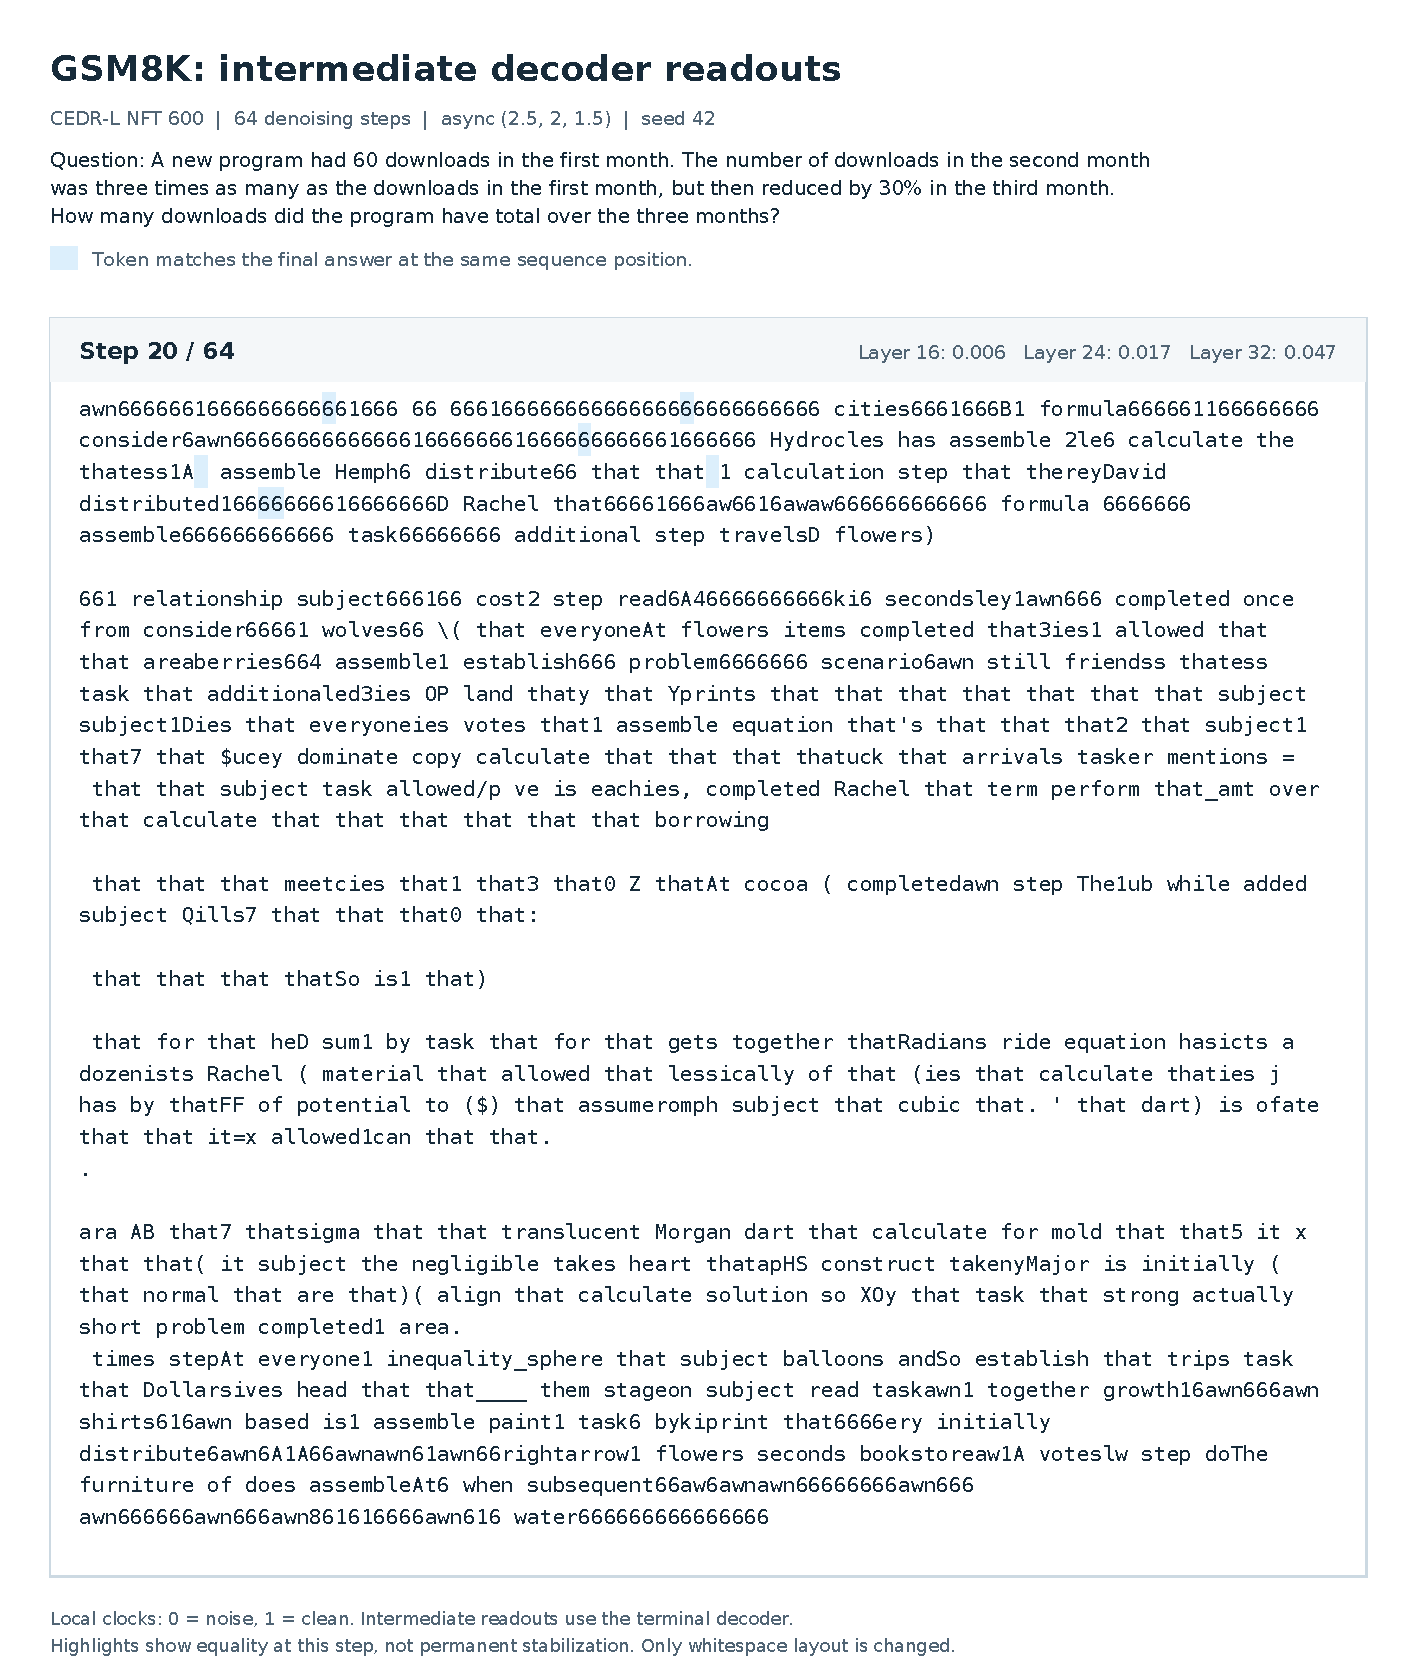
\includegraphics[width=\linewidth,height=0.84\textheight,keepaspectratio]{figures/gsm8k_trajectory_rerun_steps20.pdf}
\caption{\textbf{GSM8K generation trajectory: step 20.} Early decoder readout for the example in Figure~\ref{fig:headlineexamples}. CEDR-L NFT update 600; backbone/prompt EMA $.99/.99$; seed 42; async $(2.5,2,1.5)$; 64 denoising steps; CFG~1 and SCCFG~2. Light blue identifies tokens matching the final answer at the same position.}
\label{fig:gsmtrajectory}
\end{figure}

\begin{figure}[p]
\centering
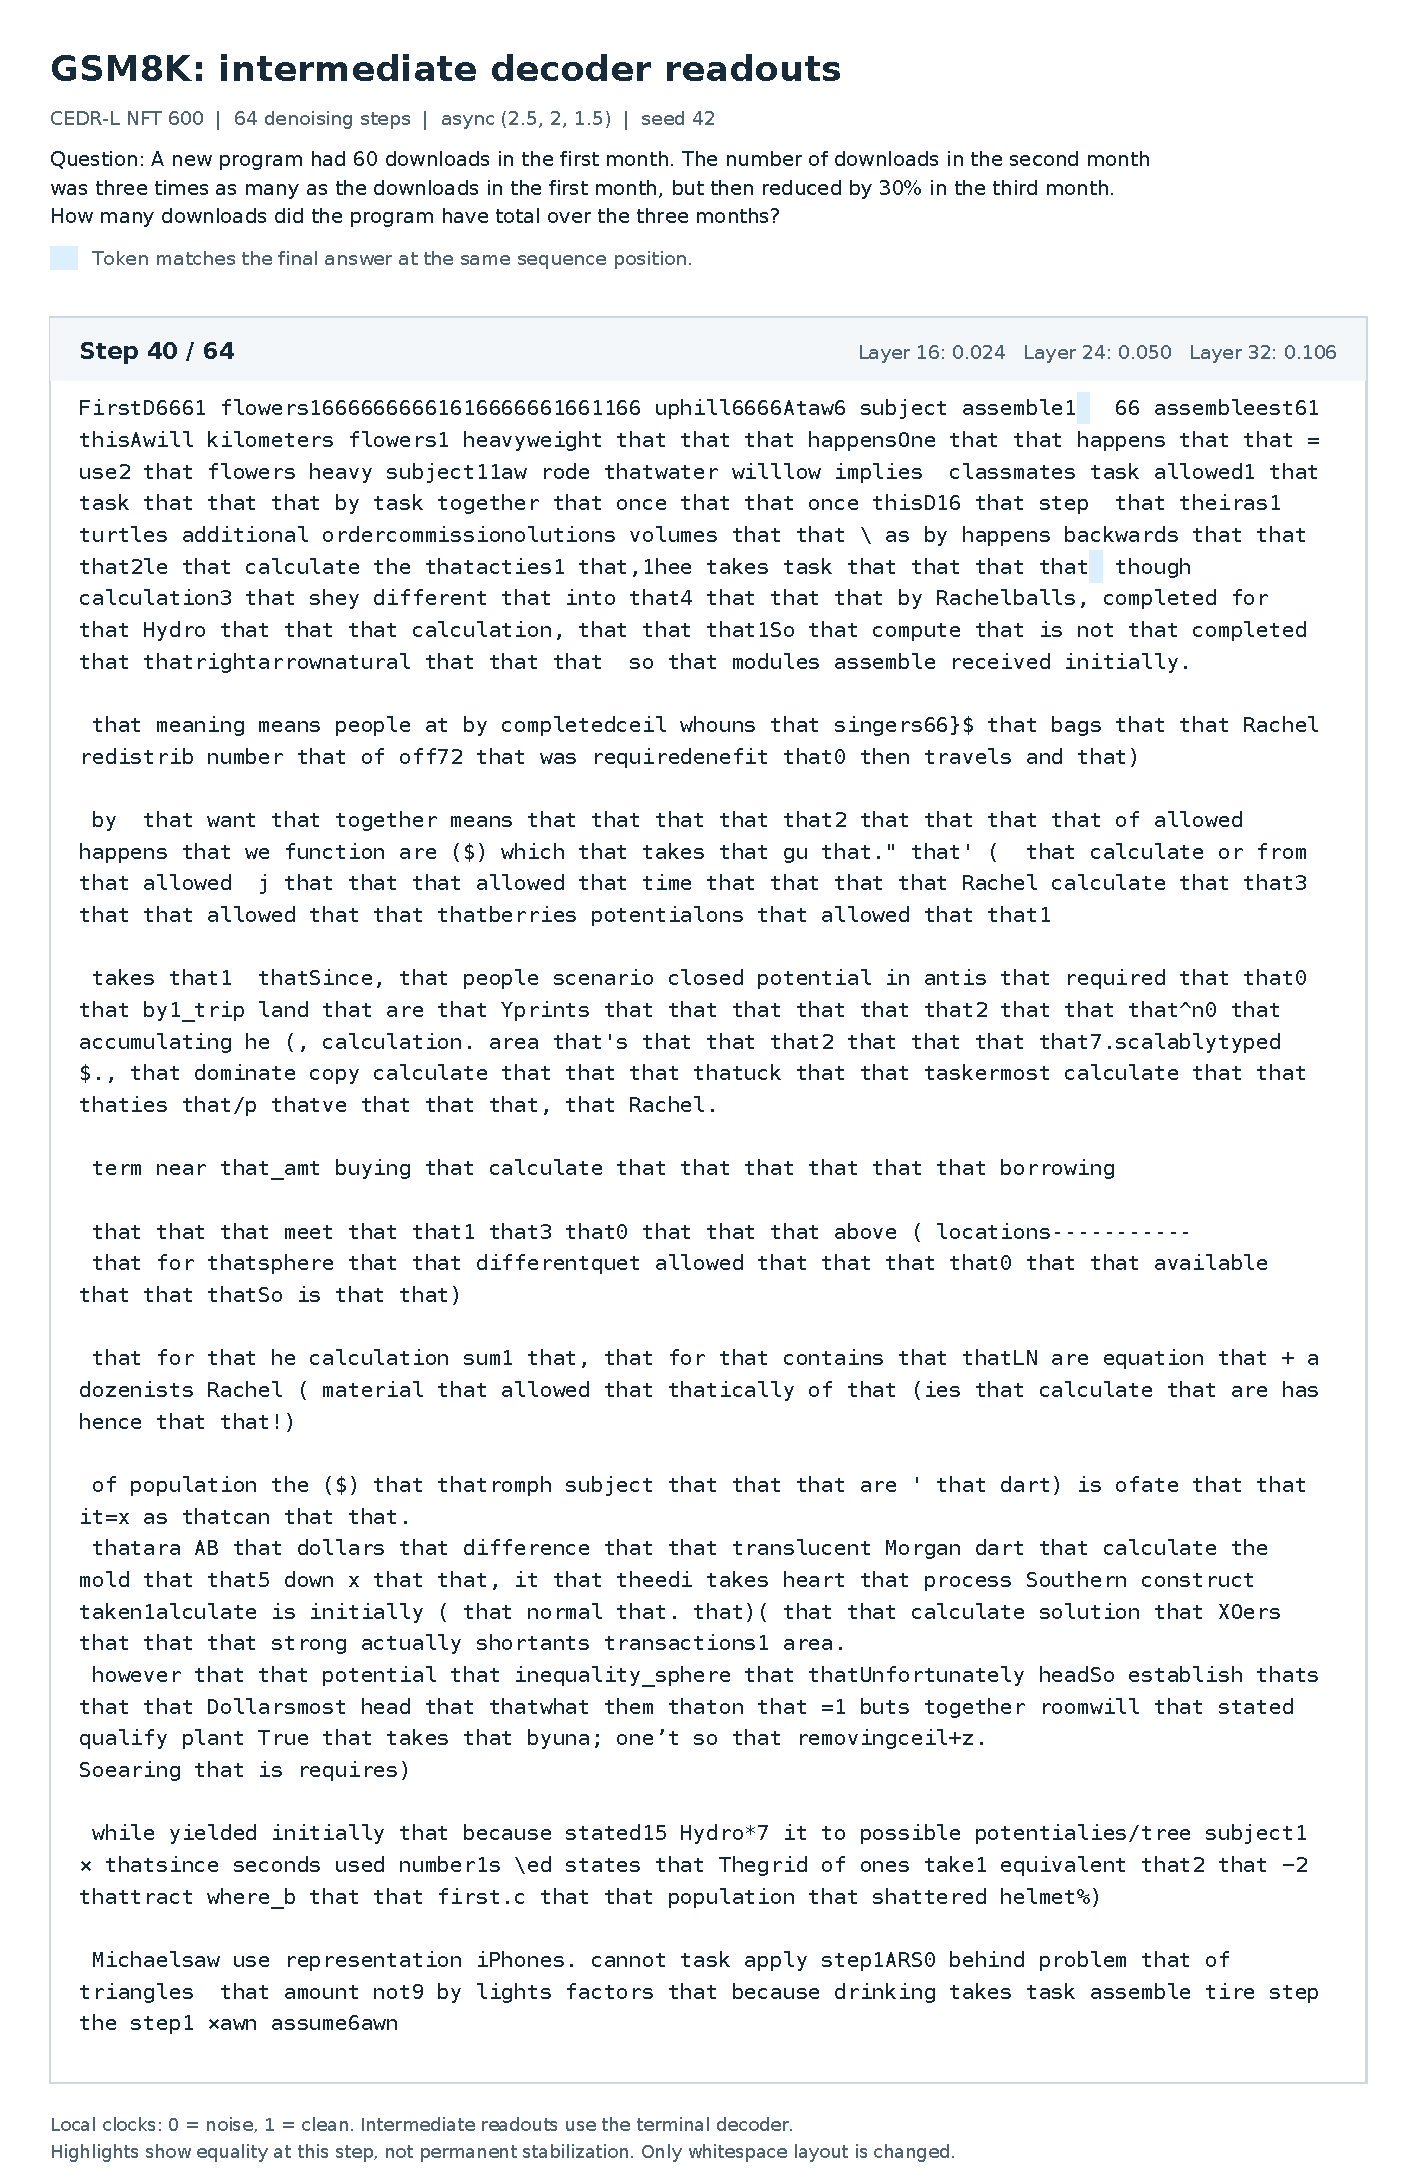
\includegraphics[width=\linewidth,height=0.84\textheight,keepaspectratio]{figures/gsm8k_trajectory_rerun_steps40.pdf}
\caption{\textbf{GSM8K generation trajectory: step 40.} The same example and settings as Figure~\ref{fig:gsmtrajectory}, with positional final-token matches highlighted in light blue.}
\label{fig:gsmtrajectory40}
\end{figure}

\begin{figure}[p]
\centering
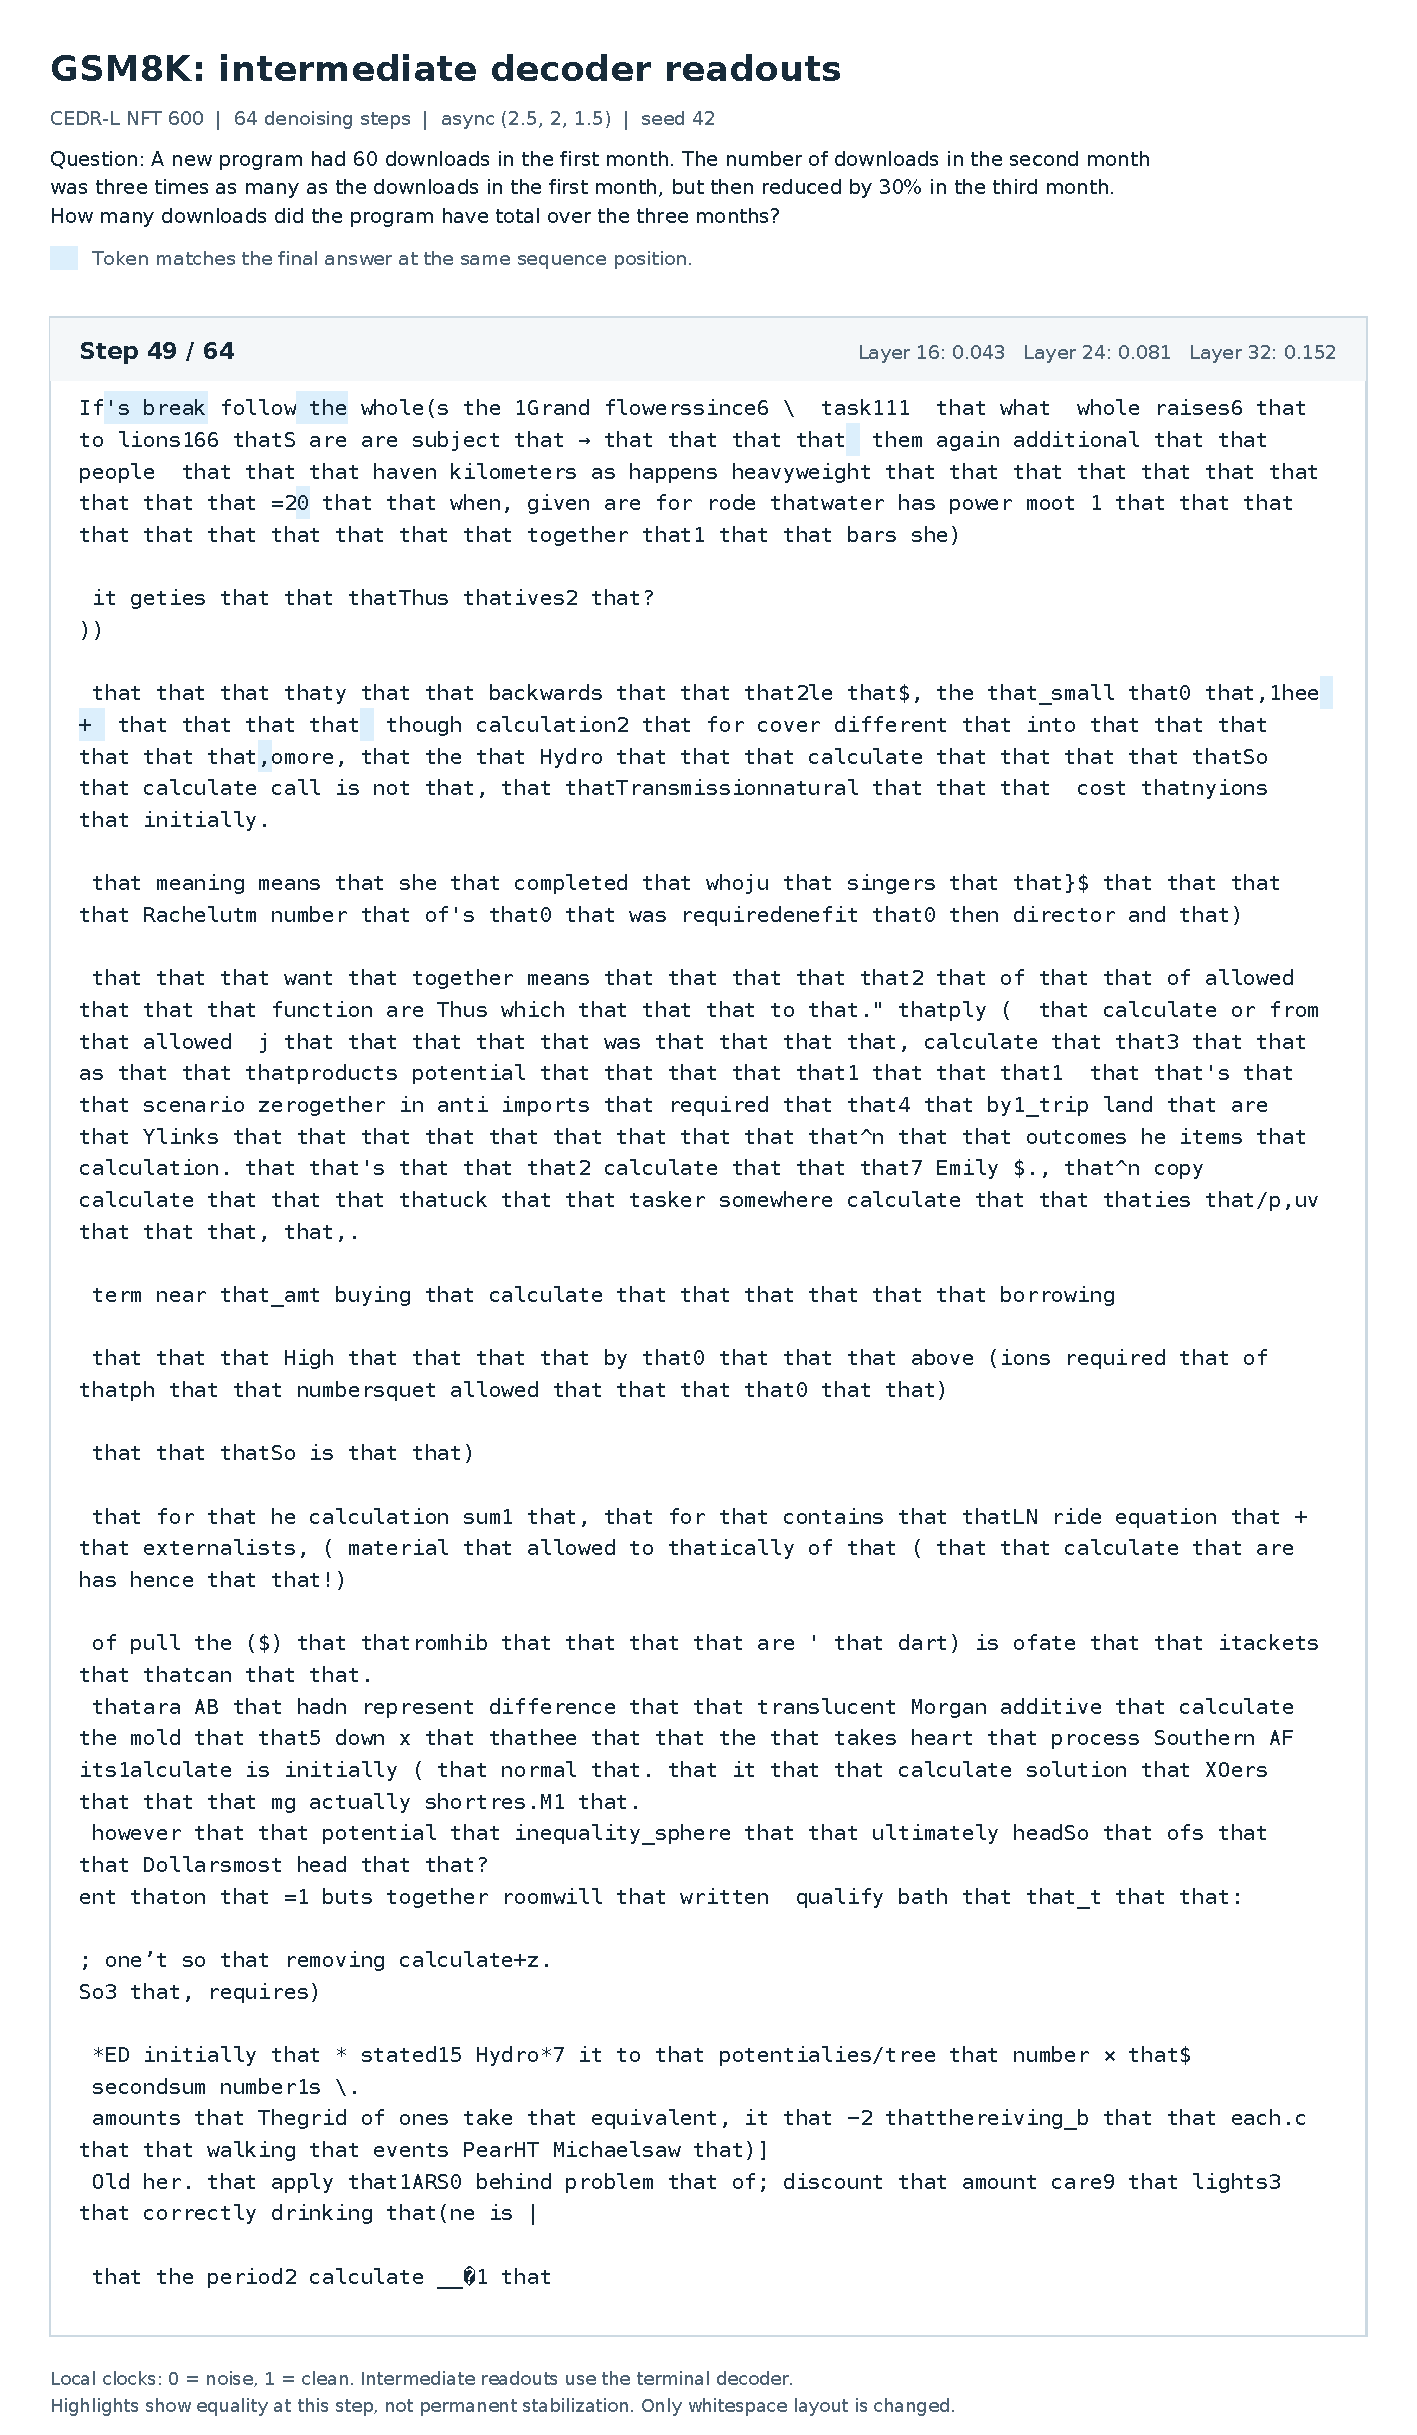
\includegraphics[width=\linewidth,height=0.84\textheight,keepaspectratio]{figures/gsm8k_trajectory_rerun_steps49.pdf}
\caption{\textbf{GSM8K generation trajectory: step 49.} The same example and settings as Figure~\ref{fig:gsmtrajectory}, with positional final-token matches highlighted in light blue.}
\label{fig:gsmtrajectory49}
\end{figure}

\begin{figure}[p]
\centering
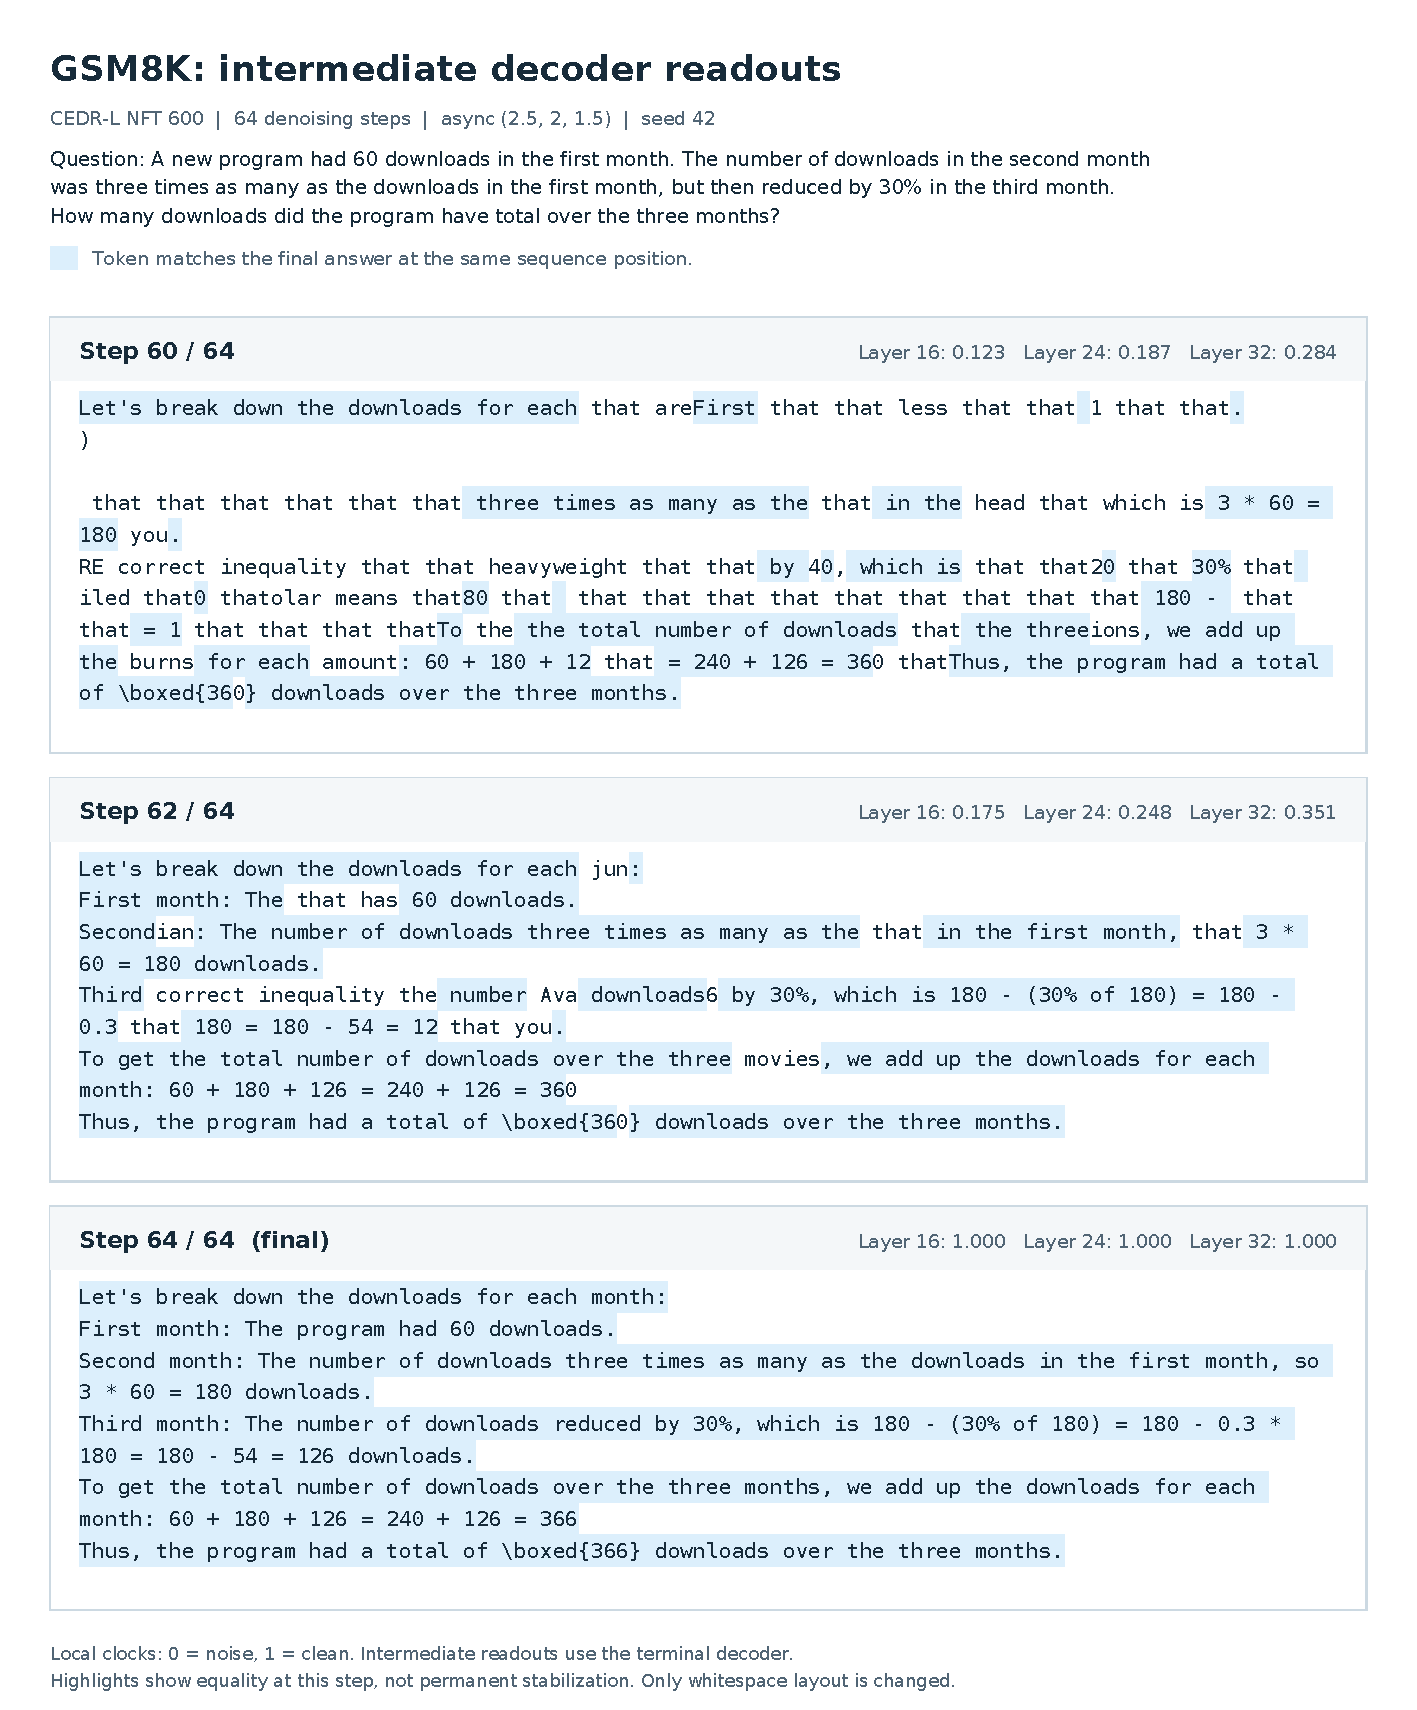
\includegraphics[width=\linewidth,height=0.84\textheight,keepaspectratio]{figures/gsm8k_trajectory_rerun_steps60_62_64.pdf}
\caption{\textbf{GSM8K generation trajectory: steps 60, 62, and 64.} Later readouts for the same example and settings as Figure~\ref{fig:gsmtrajectory}, with the final solution in the bottom panel.}
\label{fig:gsmtrajectoryfinal}
\end{figure}

\end{document}
